\chapter{HASIL DAN PEMBAHASAN}

\section{Perancangan \textit{(Exploration Phase)}}

\subsection{\textit{Requirements}}

Pada fase ini, seluruh kebutuhan pengguna akan dikumpulkan dalam bentuk \textit{user story}. Seluruh \textit{user story} akan diubah menjadi \textit{task} yang dapat dikerjakan pada jangka waktu tertentu yang disebut dengan iterasi. Pada metode \textit{Extreme Programming}, iterasi dapat berlangsung selama 1 hingga 2 pekan. Dalam penelitian ini, 1 iterasi akan ditetapkan berlangsung selama 1 pekan. \textit{User story} pada penelitian ini dapat dilihat pada tabel dibawah.

\begin{longtable}[!h]
    {
            p{0.15\textwidth}
            p{0.15\textwidth}
            p{0.35\textwidth}
            p{0.35\textwidth}
    }
    \caption{Daftar \textit{user story} Sistem Monitoring}
    \label{tab:user-story-fix} \\

    \hline
        \bfseries \textit{Code} &
        \bfseries \textit{Persona} &
        \bfseries \textit{I want to} &
        \bfseries \textit{So that can} \\ [0.5ex]
    \hline

    \endfirsthead

    \hline
        \bfseries \textit{Code} &
        \bfseries \textit{Persona} &
        \bfseries \textit{I want to} &
        \bfseries \textit{So that can} \\ [0.5ex]
    \hline
    \endhead % all the lines above this will be repeated on every page
    \hline

    \csvreader[
        late after line=\\,
        before reading={\catcode`\#=12},after reading={\catcode`\#=6}
    ]{tables/hasil/user-story.csv}{1=\K, 2=\P, 3=\I, 4=\S}{\K & \P & \I & \S} \\

    \bottomrule
\end{longtable}

\subsection{Architecture Modelling}

Dalam buku \textit{Fundamental of Software Architecture} oleh \textcite{book:richard}, arsitektur didefinisikan sebagai sebuah rangkaian dari keputusan yang akan menentukan struktur dan perilaku sistem. Pada metode XP, model arsitektur dibuat untuk mempertimbangkan berbagai solusi alternatif. Model arsitektur pada Sistem Monitoring dapat dilihat pada Gambar \ref{fig:archi-model-sm} .

\begin{figure}[!h]
    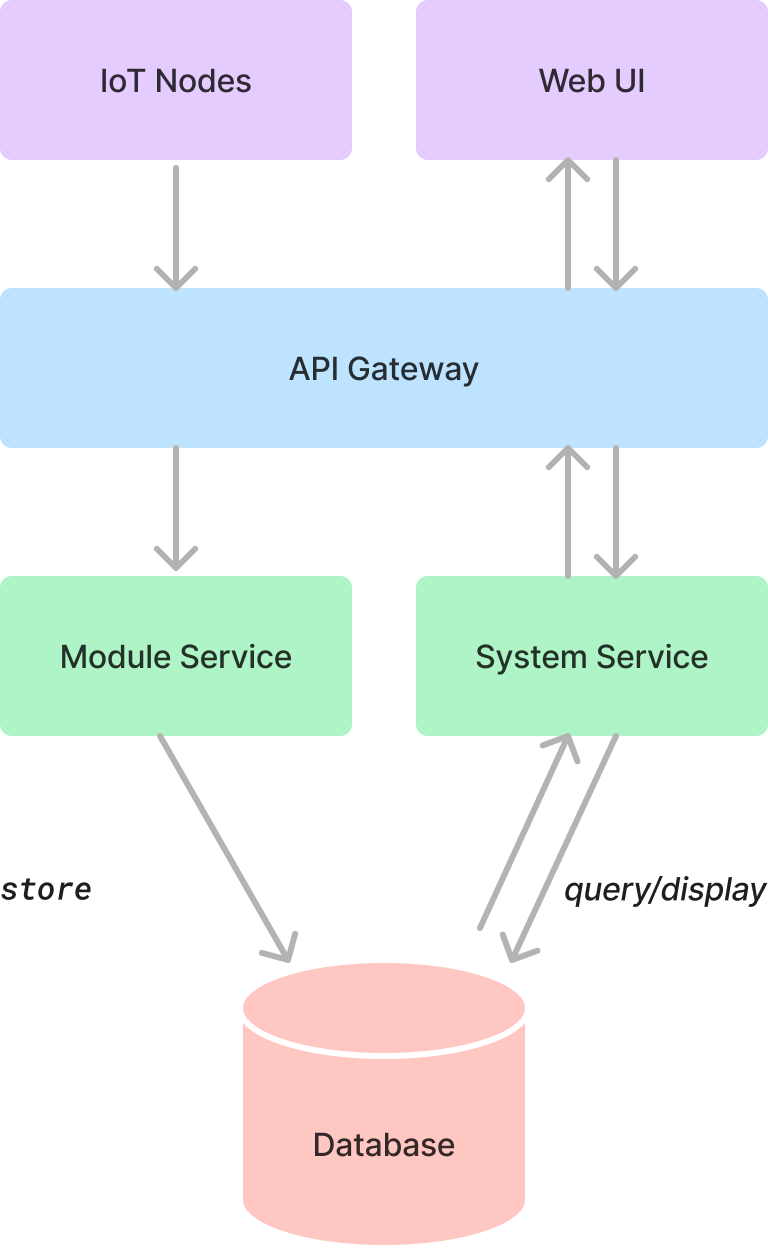
\includegraphics[width=.4\linewidth, center]{images/hasil/archi-model.png}
    \caption{Metafor Model Arsitektur Sistem Monitoring}
    \label{fig:archi-model-sm}
\end{figure}

Gambar \ref{fig:archi-model-sm} merupakan model arsitektur dengan style \textit{Service-based Architecture} dengan pertimbangan bahwa sistem tidak hanya menyediakan \textit{(API Gateway)} untuk web dasbor saja, melainkan juga untuk perangkat IoT yang akan dipasang di kapal, disebut juga dengan \textit{IoT Nodes}. \textit{IoT Nodes} dapat mengirimkan data ke server melalui \textit{(API Gateway)} yang telah diatur pada \textit{Module Service} untuk meneruskan data ke \textit{Database}. Data yang telah tersimpan dapat diakses melalui \textit{Web UI} yang terhubung dengan \textit{System Service} melalui \textit{(API Gateway)}. Selain mengakses data, sistem juga memungkinkan pengguna untuk dapat melakukan filter data dengan memberi input tanggal yang ditunjukkan oleh dua garis penghubung pada setiap obyek yang menghubungkan \textit{Web UI} dengan \textit{Database}.

\subsection{Tools dan Teknologi}

Selama pengembangan sistem, digunakan beberapa \textit{tools} yang akan membantu proses tersebut serta pemilihan teknologi \textit{(techstack)} untuk Sistem Monitoring yang sebelumnya telah dibahas pada Bab 2 dan Bab 3. Untuk tools yang digunakan dalam penelitian ini meliputi VSCode sebagai IDE, phpmyadmin untuk melakukan manajemen basis data, Figma untuk mendesain arsitektur, skema basis data, dan prototype, serta Apidog untuk pengujian API.

\section{Perencanaan \textit{(Planning)}}

Pada tahap ini, seluruh \textit{User Story} akan menjadi kumpulan \textit{task} yang akan disortir berdasarkan tingkat prioritas yang dinilai dari 1 hingga 5 dan estimasi waktu pengerjaannya dalam satuan hari. Seluruh rencana iterasi dapat dilihat pada Tabel \ref{tab:iteration-1} hingga Tabel \ref{tab:iteration-5} dibawah.

Iterasi pertama difokuskan untuk mengelola data kecepatan mesin dan menampilkannya dalam bentuk grafik.

\begin{longtable}[!h]
    {
            p{0.2\textwidth}
            p{0.4\textwidth}
            >{\centering\arraybackslash}p{0.15\textwidth}
            >{\centering\arraybackslash}p{0.15\textwidth}
    }
    \caption{Rencana Iterasi 1}
    \label{tab:iteration-1} \\

    \hline
        \bfseries \textit{Kode User Story} &
        \bfseries \textit{Deskripsi Task} &
        \bfseries \textit{Prioritas} &
        \bfseries \textit{Estimasi Waktu} \\ [0.5ex]
    \hline

    \endfirsthead

    \hline
        \bfseries \textit{Kode User Story} &
        \bfseries \textit{Deskripsi} &
        \bfseries \textit{Prioritas} &
        \bfseries \textit{Estimasi Waktu} \\ [0.5ex]
    \hline
    \endhead % all the lines above this will be repeated on every page
    \hline

    \csvreader[
        late after line=\\,
        before reading={\catcode`\#=12},after reading={\catcode`\#=6}
    ]{tables/hasil/iterations/1/task.csv}
    {1=\K, 2=\D, 3=\P, 4=\T}{\K & \D & \P & \T} \\

    \bottomrule
\end{longtable}

Pada iterasi kedua, dilanjutkan pengembangan Halaman Fuel Consumption, Running Hour, dan Data Log.

\begin{longtable}[!h]
    {
            p{0.15\textwidth}
            p{0.4\textwidth}
            >{\centering\arraybackslash}p{0.15\textwidth}
            >{\centering\arraybackslash}p{0.15\textwidth}
    }
    \caption{Rencana Iterasi 2}
    \label{tab:iteration-2} \\

    \hline
        \bfseries Kode User Story &
        \bfseries Deskripsi Task &
        \bfseries Prioritas &
        \bfseries Estimasi Waktu \\ [0.5ex]
    \hline

    \endfirsthead

    \hline
        \bfseries Kode User Story &
        \bfseries Deskripsi &
        \bfseries Prioritas &
        \bfseries Estimasi Waktu \\ [0.5ex]
    \hline
    \endhead % all the lines above this will be repeated on every page
    \hline

    \csvreader[
        late after line=\\,
        before reading={\catcode`\#=12},after reading={\catcode`\#=6}
    ]{tables/hasil/iterations/2/task.csv}
    {1=\c, 2=\d, 3=\p, 4=\t}{\c & \d & \p & \t} \\

    \bottomrule
\end{longtable}

Selanjutnya, pada iterasi ketiga dilakukan pengembangan sistem admin yang memungkinkan pengguna melakukan manajemen data seperti data pengguna, data kapal, dan data batas kecepatan pada setiap kategori operasional FCRV.

\begin{longtable}[!h]
    {
            p{0.15\textwidth}
            p{0.4\textwidth}
            >{\centering\arraybackslash}p{0.15\textwidth}
            >{\centering\arraybackslash}p{0.15\textwidth}
    }
    \caption{Rencana Iterasi 3}
    \label{tab:iteration-3} \\

    \hline
        \bfseries Kode User Story &
        \bfseries Deskripsi Task &
        \bfseries Prioritas &
        \bfseries Estimasi Waktu \\ [0.5ex]
    \hline

    \endfirsthead

    \hline
        \bfseries Kode User Story &
        \bfseries Deskripsi &
        \bfseries Prioritas &
        \bfseries Estimasi Waktu \\ [0.5ex]
    \hline
    \endhead % all the lines above this will be repeated on every page
    \hline

    \csvreader[
        late after line=\\,
        before reading={\catcode`\#=12},after reading={\catcode`\#=6}
    ]{tables/hasil/iterations/3/task.csv}
    {1=\c, 2=\d, 3=\p, 4=\t}{\c & \d & \p & \t} \\

    \bottomrule
\end{longtable}

Iterasi keempat berfokus pada halaman Overview, ekspor data mentah kecepatan mesin dalam format CSV, dan laporan harian kecepatan mesin dan konsumsi bahan bakar dalam format PDF

\begin{longtable}[!h]
    {
            p{0.15\textwidth}
            p{0.4\textwidth}
            >{\centering\arraybackslash}p{0.15\textwidth}
            >{\centering\arraybackslash}p{0.15\textwidth}
    }
    \caption{Rencana Iterasi 4}
    \label{tab:iteration-4} \\

    \hline
        \bfseries Kode User Story &
        \bfseries Deskripsi Task &
        \bfseries Prioritas &
        \bfseries Estimasi Waktu \\ [0.5ex]
    \hline

    \endfirsthead

    \hline
        \bfseries Kode User Story &
        \bfseries Deskripsi &
        \bfseries Prioritas &
        \bfseries Estimasi Waktu \\ [0.5ex]
    \hline
    \endhead % all the lines above this will be repeated on every page
    \hline

    \csvreader[
        late after line=\\,
        before reading={\catcode`\#=12},after reading={\catcode`\#=6}
    ]{tables/hasil/iterations/4/task.csv}
    {1=\c, 2=\d, 3=\p, 4=\t}{\c & \d & \p & \t} \\

    \bottomrule
\end{longtable}

Terakhir, pada iterasi kelima dilakukan pengembangan halaman OP41 Report, halaman Home, dan sistem autentikasi.

\begin{longtable}[!h]
    {
            p{0.2\textwidth}
            p{0.4\textwidth}
            >{\centering\arraybackslash}p{0.15\textwidth}
            >{\centering\arraybackslash}p{0.15\textwidth}
    }
    \caption{Rencana Iterasi 5}
    \label{tab:iteration-5} \\

    \hline
        \bfseries \textit{Kode User Story} &
        \bfseries \textit{Deskripsi Task} &
        \bfseries \textit{Prioritas} &
        \bfseries \textit{Estimasi Waktu} \\ [0.5ex]
    \hline

    \endfirsthead

    \hline
        \bfseries \textit{Kode User Story} &
        \bfseries \textit{Deskripsi} &
        \bfseries \textit{Prioritas} &
        \bfseries \textit{Estimasi Waktu} \\ [0.5ex]
    \hline
    \endhead % all the lines above this will be repeated on every page
    \hline

    \csvreader[
        late after line=\\,
        before reading={\catcode`\#=12},after reading={\catcode`\#=6}
    ]{tables/hasil/iterations/5/task.csv}
    {1=\K, 2=\D, 3=\P, 4=\T}{\K & \D & \P & \T} \\

    \bottomrule
\end{longtable}


\section{Implementasi \textit{(Iteration to Release)}}

\begin{figure}[!h]
    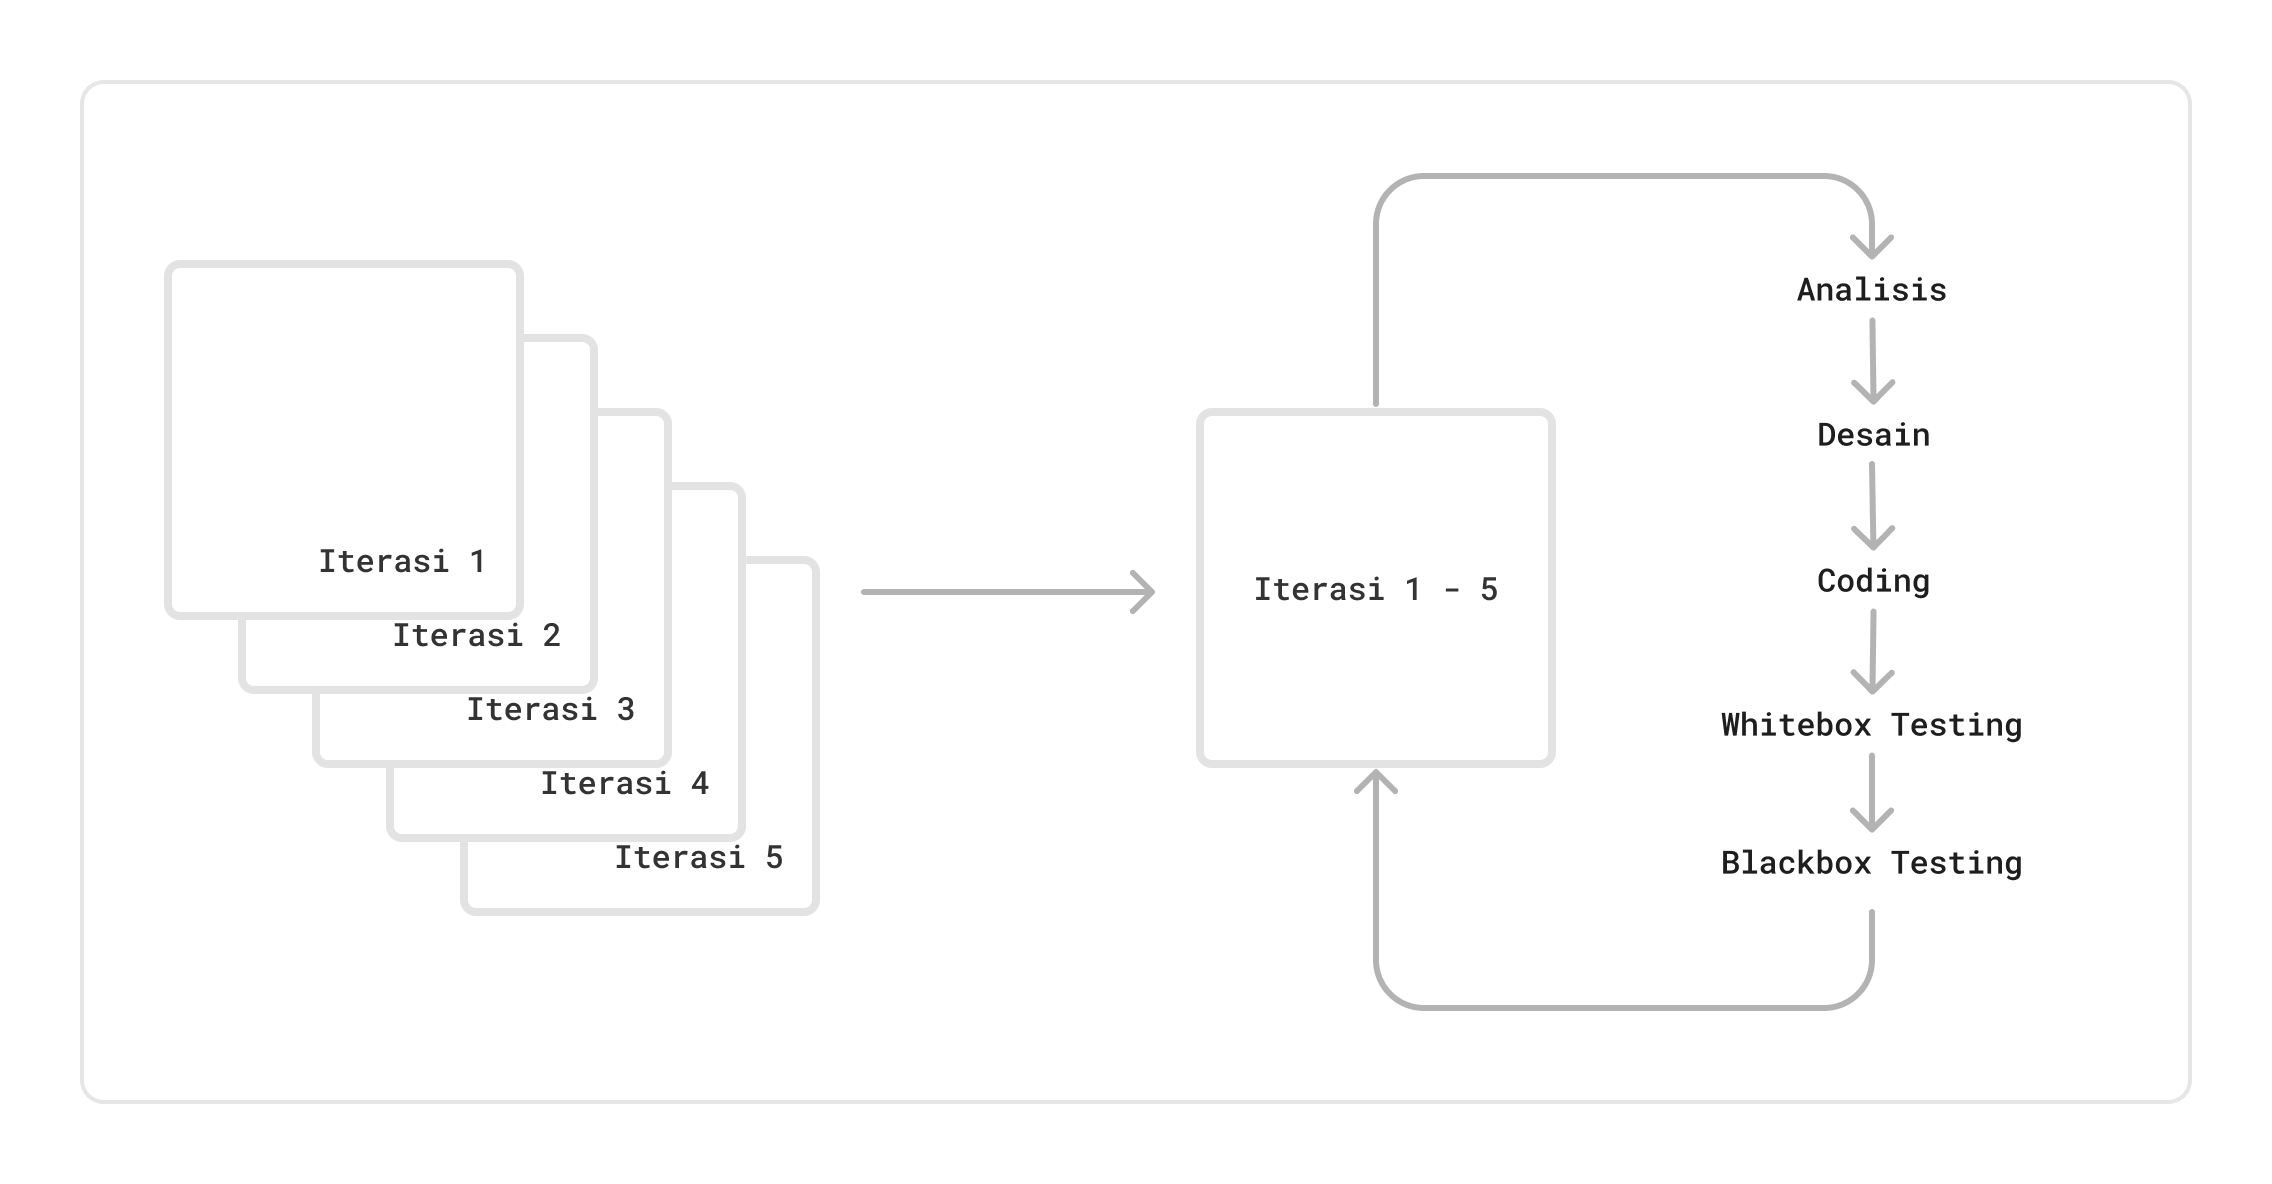
\includegraphics[width=1.05\linewidth, center]{images/hasil/overview.png}
    \caption{Garis Besar Pengerjaan Implementasi}
    \label{fig:imp-overview}
\end{figure}

Secara garis besar, implementasi dilakukan sebanyak 5 iterasi yang berlangsung selama 5 pekan seperti yang terlihat pada Gambar \ref{fig:imp-overview}. Dimulai dari tahap analisis yang akan menghasilkan kebutuhan sistem, dilanjutkan dengan perancangan \textit{wireframe} sebagai acuan pada pengembangan antarmuka di fase koding, yang akan melewati serangkaian proses pengujian yang disebut dengan \textit{Whitebox Testing} dan \textit{Blackbox Testing}. Pengujian \textit{whitebox} dilakukan untuk memastikan kesesuaian seluruh struktur dan logika pemrograman dengan melalui \textit{unit test}. Lalu, setelahnya dilakukan pengujian langsung oleh mitra untuk memastikan input dan output sistem telah sesuai.

Setelah satu iterasi selesai dan telah melewati seluruh ceklis pada \textit{Whitebox} dan \textit{Blackbox testing} maka akan dilanjutkan ke iterasi kedua. Pada penelitian ini, hasil iterasi 2 hingga iterasi 5 ditaruh pada lampiran dikarenakan memiliki pola pengembangan yang identikal. Hasil pada iterasi 1 akan secara detail dijabarkan pada bagian-bagian berikut.

\subsection{\textit{Analysis}}

Kebutuhan sistem merupakan analisis yang dilakukan untuk mengetahui kebutuhan fungsional sistem. Kebutuhan fungsional sistem sendiri merupakan fungsionalitas yang harus tersedia di sistem sesuai kebutuhan \textit{stakeholder} yang tertuang di \textit{user story}. Aturan penomoran kebutuhan sistem dapat dilihat pada Tabel \ref{tab:aturan-penomoran} .

\begin{table}[!h]
    \caption{Aturan Penomoran Kebutuhan Sistem}
    \centering
    \begin{tabular}
        {
            >{\centering\arraybackslash}p{0.2\textwidth}
            >{\centering\arraybackslash}p{0.4\textwidth}
        }
        \toprule

        Kode &
        Keterangan \\ [1ex]

        \midrule

        SM- & Sistem Monitoring \\
        -F- & Kebutuhan Fungsional \\
        -\{x\} & Nomor Urutan Kode Kebutuhan \\

        \bottomrule
    \end{tabular}
    \label{tab:aturan-penomoran}
\end{table}

\newpage

Berikut merupakan contoh kebutuhan fungsional pada iterasi 1 yang hanya meliputi fitur Engine Speed saja dikarenakan estimasi waktu pengerjaan yang memakan waktu relatif lebih lama. Kebutuhan fungsional memuat setidaknya kode fungsional, nama fitur, pengguna, serta deskripsi dan spesifikasi.

\begin{figure}[!h]
    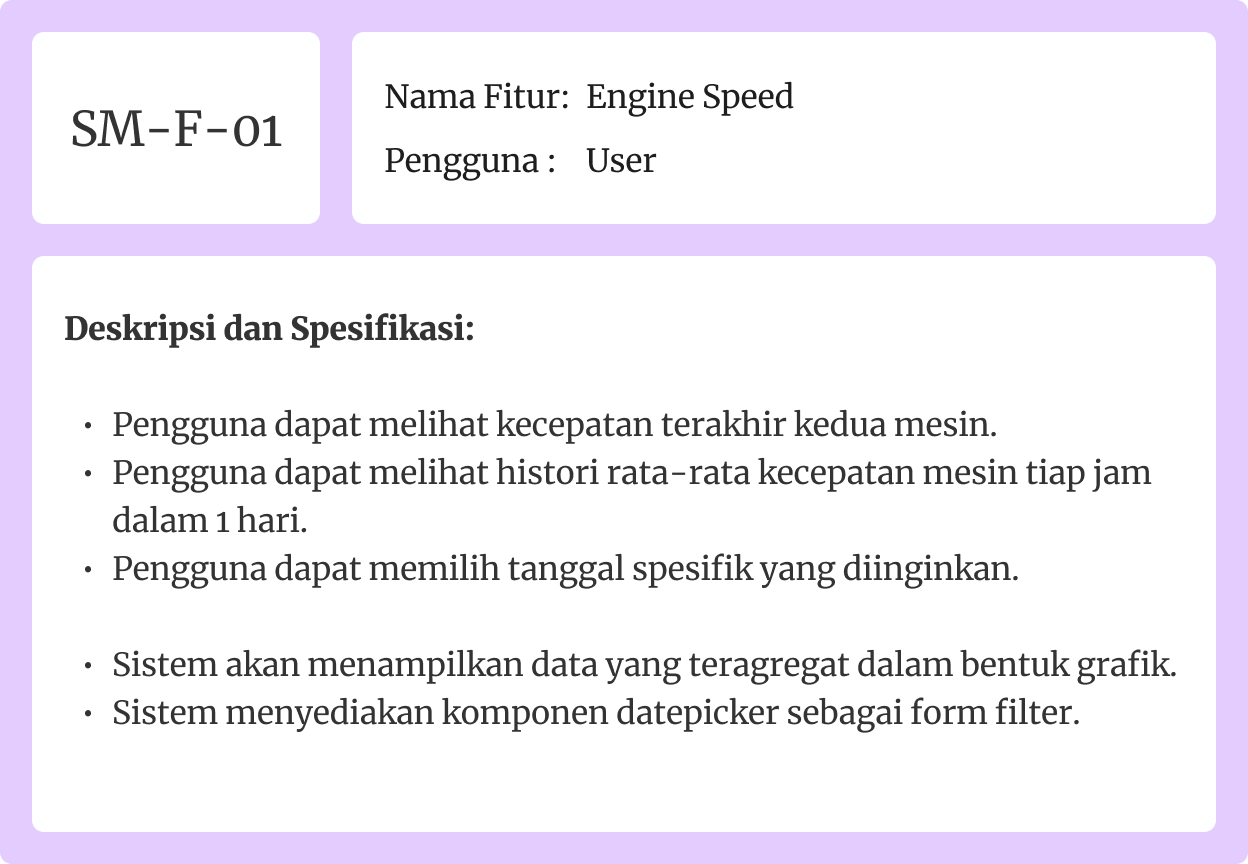
\includegraphics[width=.8\linewidth, center]{images/hasil/iterations/1/fr-es.png}
    \caption{Kebutuhan Fungsional Engine Speed}
    \label{fig:fr-es}
\end{figure}

\subsection{\textit{Design}}

Lalu, pada tahap desain dilakukan perancangan \textit{wireframe low fidelity} untuk memberikan gambaran pada pengembang terkait antarmuka dari \textit{task} yang dikerjakan. \textit{Wireframe} terdiri dari komponen dan tata letaknya tanpa teks atau konten detail. \textit{Wireframe} pada Halaman Engine Speed sendiri sebelumnya telah ditampilkan pada Gambar \ref{fig:wireframe}.

Dari \textit{wireframe} tersebut, dilakukan pengerjaan tampilan yang disebut juga dengan \textit{UI Slicing}. Pada halaman ini, pengguna dapat melihat angka kecepatan mesin terakhir dan nilai rata-rata dengan interval 1 jam dalam jangka waktu satu hari yang disajikan dalam bentuk grafik. Jangka waktu dapat dipilih melalui filter yang akan disediakan pada area komponen grafik. Seluruh navigasi pada sistem dapat dilakukan dengan memilih komponen \textit{Navbar} atau \textit{Sidebar}. Hasil pengerjaan \textit{UI Slicing} dapat dilihat pada Gambar \ref{fig:fe-es}.

\begin{figure}[!h]
    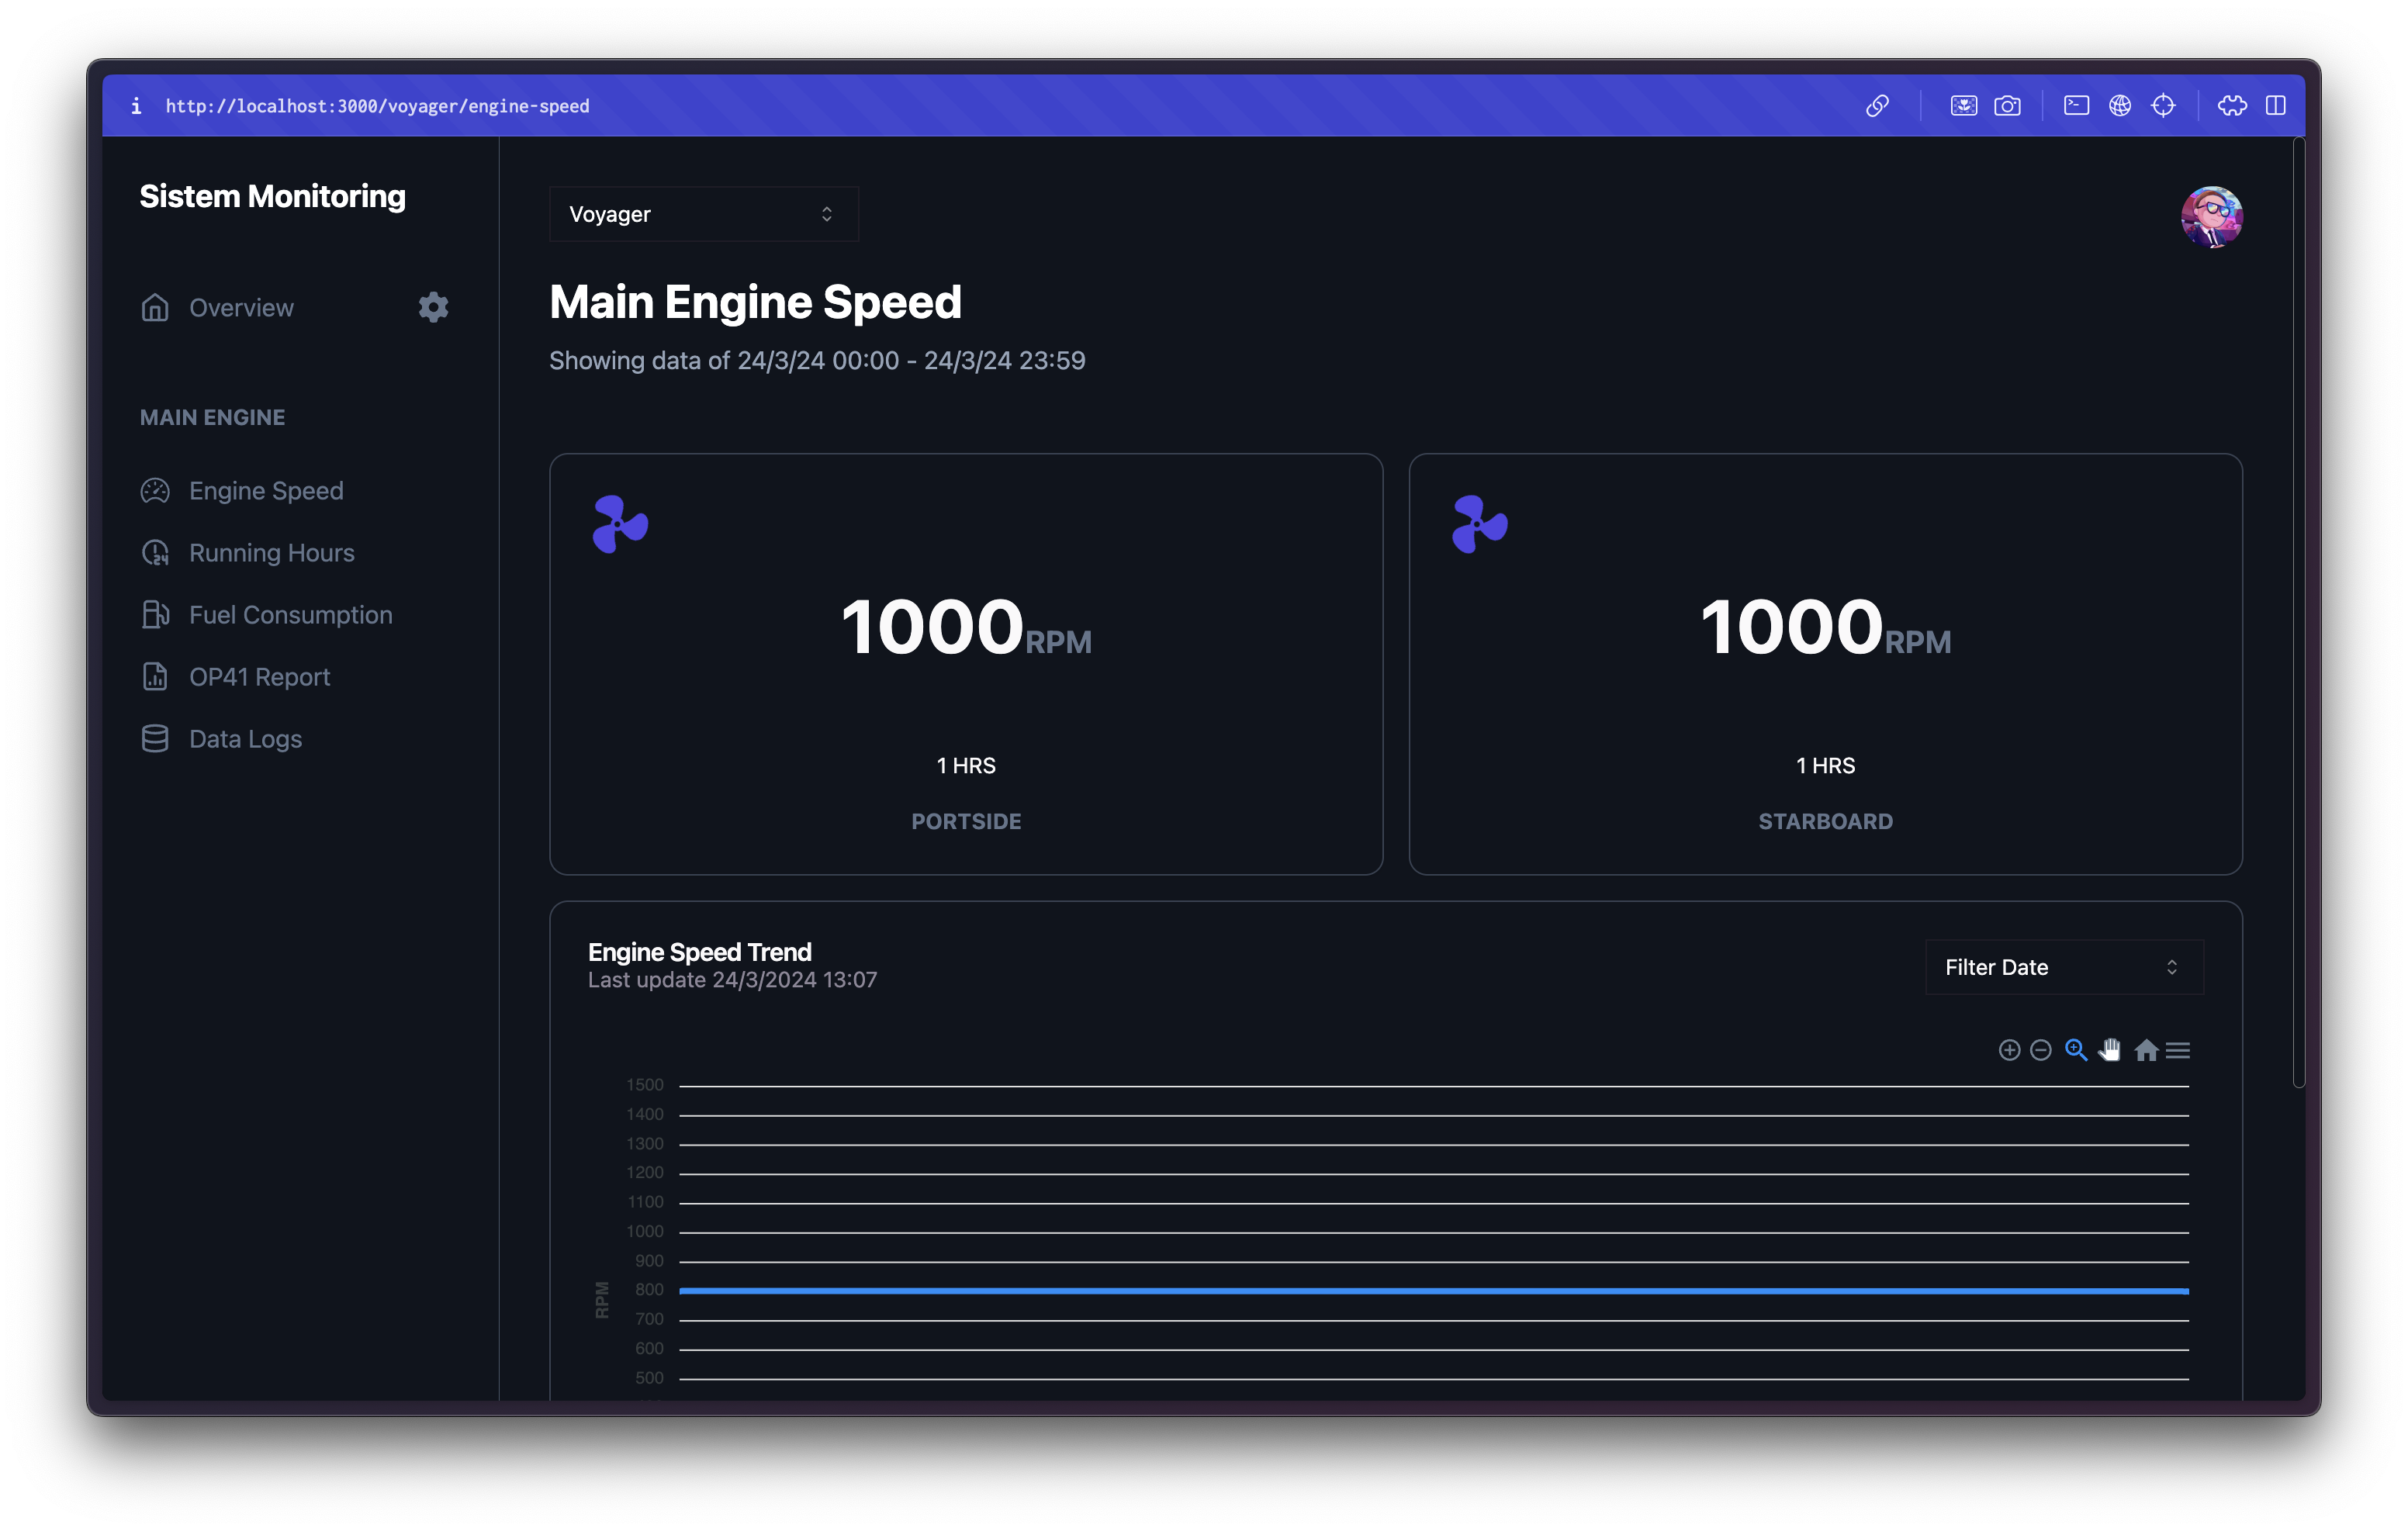
\includegraphics[width=1.05\linewidth, center]{images/hasil/iterations/1/fe-es.png}
    \caption{Frontend Halaman Engine Speed}
    \label{fig:fe-es}
\end{figure}

\subsection{\textit{Coding}}

Pada tahap ini, akan dilakukan pengkodean Halaman Engine Speed yang merupakan halaman untuk melihat kecepatan mesin terakhir dan histori tren kecepatan mesin yang disajikan dalam bentuk grafik garis. Algoritma dituangkan dalam bentuk \textit{pseudocode} dan diagram alir yang akan dijabarkan sebagai berikut.

Pada Halaman Engine Speed, data diperoleh dari \textit{server} melalui API berdasarkan kode kapal \textit{(vessel code)} dan filter tanggal. Selama proses pemanggilan data, sistem akan menampilkan animasi \textit{loading} untuk menunjukkan bahwa proses sedang berlangsung. Terdapat dua kemungkinan nilai yang dikembalikan oleh server, yakni \textit{'success'} atau \textit{'error'} beserta dengan penjelasan lengkapnya. Jika \textit{'success'} maka hasil respon dari API akan diinisiasi pada variabel \textit{engine data} dan akan ditampilkan pada komponen \textit{card} dan \textit{chart}. Sebaliknya, layar eror akan ditampilkan beserta dengan kode dan pesan erornya. \textit{Pseudocode} dan diagram alir penampilan data di Halaman Engine Speed dapat dilihat pada Tabel \ref{tab:pseudocode-fe} dan Gambar \ref{fig:flow-fe}.

\begin{longtable}[!h]
  {
          p{0.9\textwidth}
  }
  \caption{Pseudocode Halaman Engine Speed}
  \label{tab:pseudocode-fe} \\

  \hline
      \bfseries Pseudocode \\ [0.5ex]
  \hline

  \endfirsthead

  \hline
      \bfseries Pseudocode \\ [0.5ex]
  \hline
  \endhead % all the lines above this will be repeated on every page

  \begin{algorithmic}[1]
    \State $\Call{getInitialData}{vessel code, date filter}$
    \State $response \gets \Call{getInitialData}{vessel code, date filter}$
    \State \Output loading animation
    \If{response = 'success'}
      \State $data \gets response.data$
      \State \Output latest engine data and running hour to card component
      \State \Output engine data trend to line chart
    \Else
      \State \Output error screen
    \EndIf
  \end{algorithmic} \\

  \bottomrule
\end{longtable}

\begin{figure}[!h]
    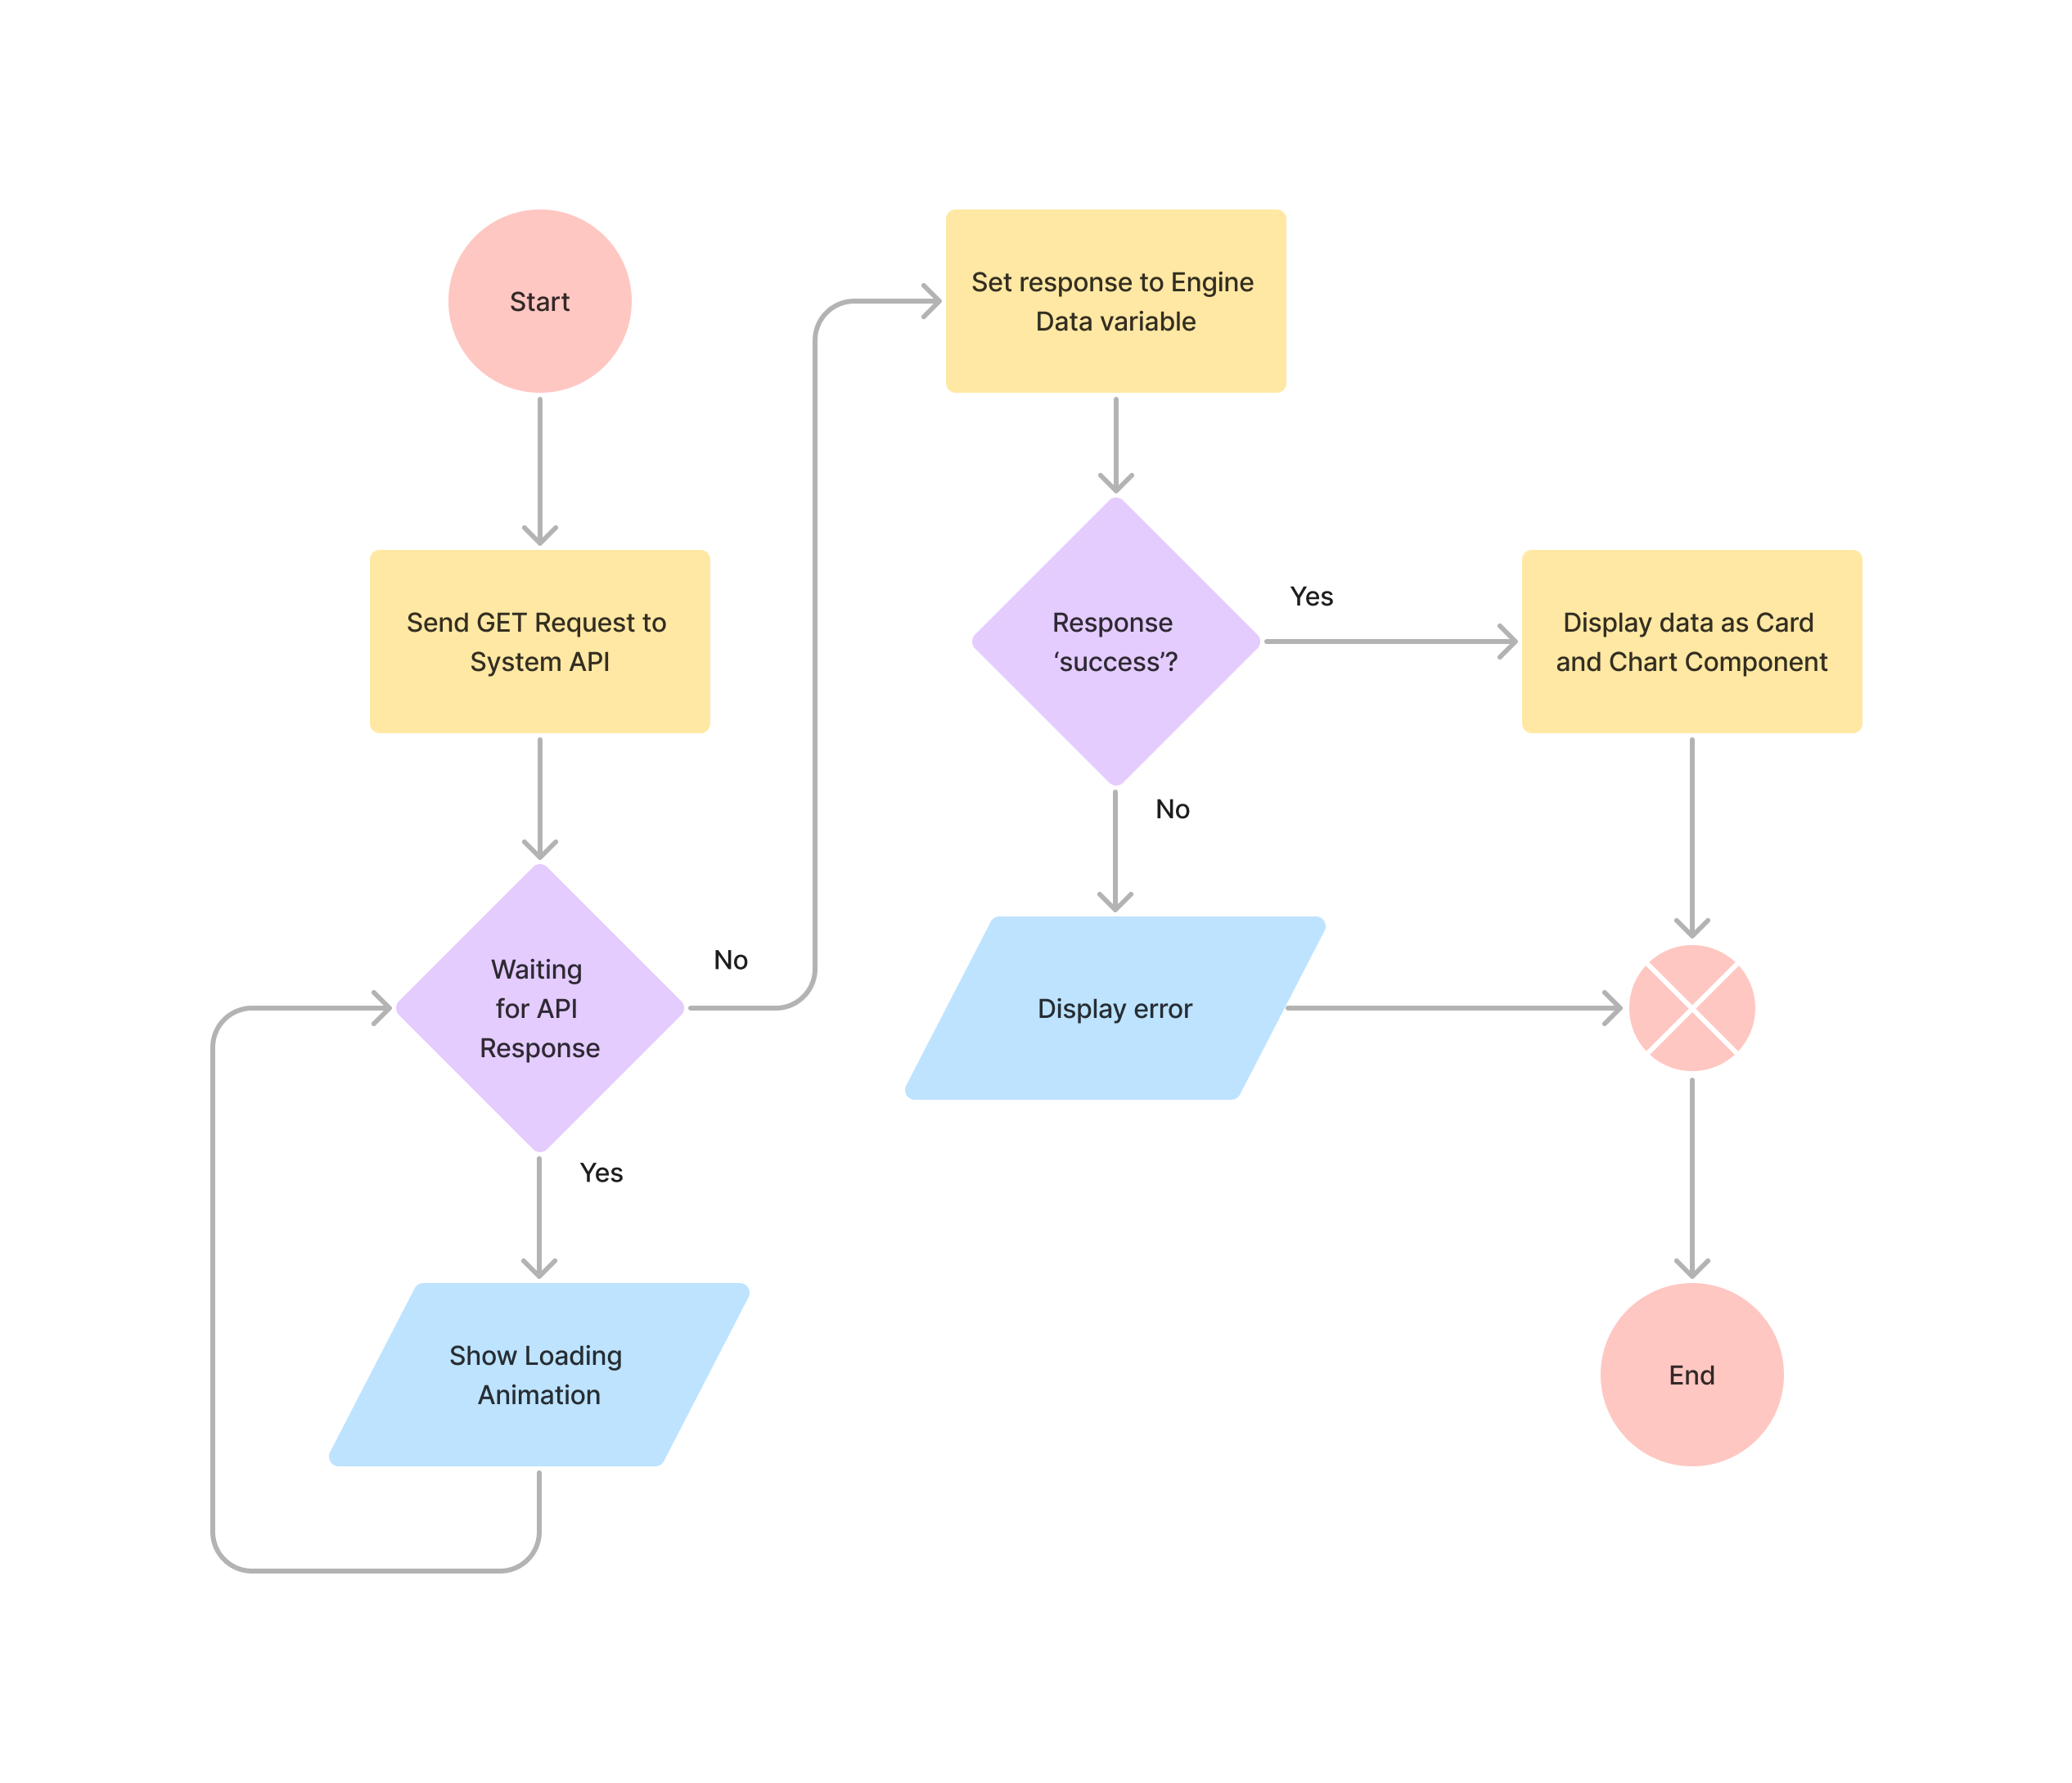
\includegraphics[width=1.2\linewidth, center]{images/flowcharts/flow-fe.png}
    \caption{Diagram Alir Halaman Engine Speed}
    \label{fig:flow-fe}
\end{figure}

\newpage

Lebih lanjut, berikut hasil dari pengerjaan Engine Speed dari sisi \textit{backend}. Pada satu \textit{endpoint}, terdapat beberapa fungsi yang dipanggil untuk mendapatkan masing-masing data seperti tanggal data terakhir, tren kecepatan mesin, kecepatan mesin terakhir, dan total running hour. Output dari fungsi-fungsi tersebut bergantung pada data kecepatan mesin yang didapatkan dari kueri. Oleh karenanya, dilakukan kontrol \textit{if statement} untuk mengecek apakah data kecepatan mesin kosong atau tidak. Jika kosong, maka fungsi akan mengembalikan nilai \textit{default} yakni 0. Diagram alir pada \textit{backend} Engine Speed dapat dilihat pada Gambar \ref{fig:flow-be-overview}.

\begin{figure}[!h]
    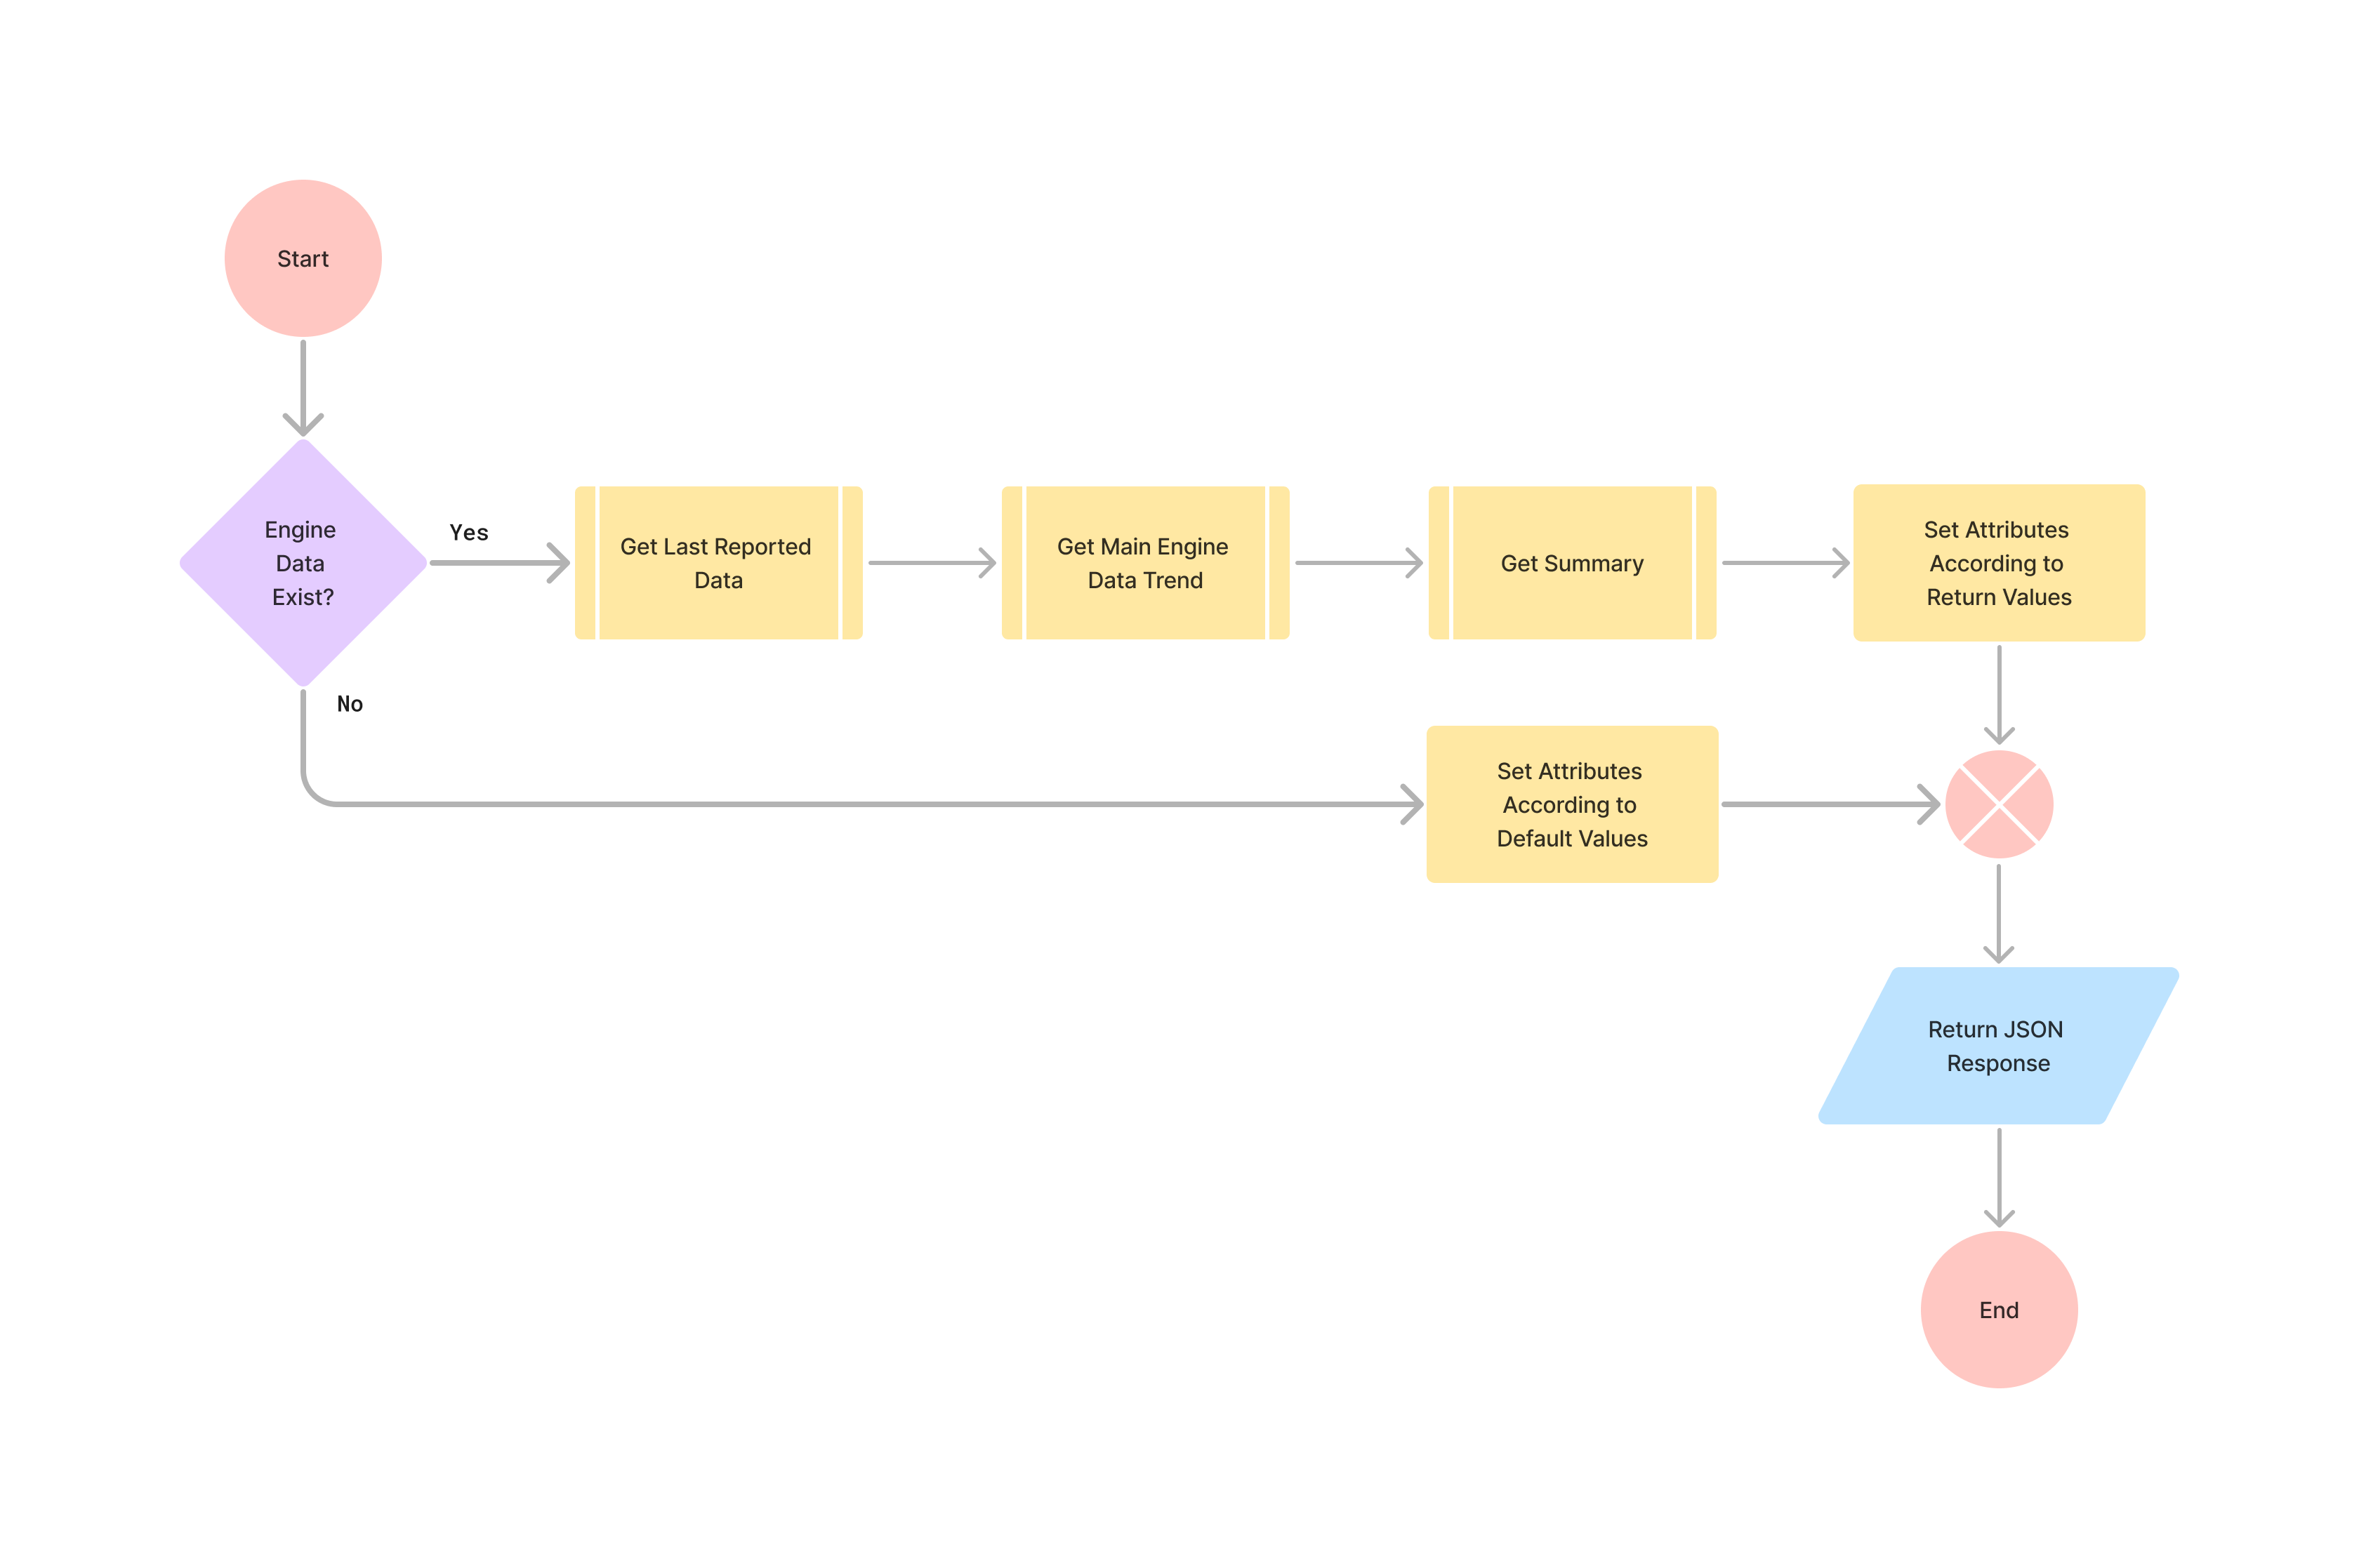
\includegraphics[width=1.2\linewidth, center]{images/flowcharts/flow-be-overview.png}
    \caption{Diagram Alir API Engine Speed}
    \label{fig:flow-be-overview}
\end{figure}

% This paragraph details the process of data collection and synchronization in the \textit{IoT Node}.
% I might not include these, since the topic is out of scope.

% Data yang ditampilkan pada web merupakan hasil pengambilan data dari \textit{IoT Node} yang sebelumnya telah terpasang di kapal. \textit{IoT Node} memiliki dua proses yang dijalankan secara simultan, yakni pengambilan data dan sinkronisasi data. Pengambilan data dilakukan setiap interval 1 menit yang berisi data kecepatan mesin kiri dan kanan serta tanggal dan waktunya. Berikut merupakan alur pengambilan data pada \textit{IoT Node} yang dapat dilihat pada Tabel \ref{tab:pseudocode-iot-node} dan Gambar \ref{fig:flow-iot-node}.

% \begin{longtable}[!h]
  {
          p{0.9\textwidth}
  }
  \caption{Pseudocode Pengambilan Data Kecepatan Mesin Pada IoT Node}
  \label{tab:pseudocode-iot-node} \\

  \hline
      \bfseries Pseudocode \\ [0.5ex]
  \hline

  \endfirsthead

  \hline
      \bfseries Pseudocode \\ [0.5ex]
  \hline
  \endhead % all the lines above this will be repeated on every page

  WHILE TRUE \\
  \hspace{5mm} READ portside speed via PWM \\
  \hspace{5mm} SET portside speed \\
  \hspace{5mm} READ starboard speed via PWM \\
  \hspace{5mm} SET starboard speed \\
  \hspace{5mm} SET datetime \\
  \hspace{5mm} WRITE engine data to local database \\
  \hspace{5mm} DELAY 60 seconds \\
  ENDWHILE \\

  \bottomrule
\end{longtable}
% \begin{figure}[!h]
%     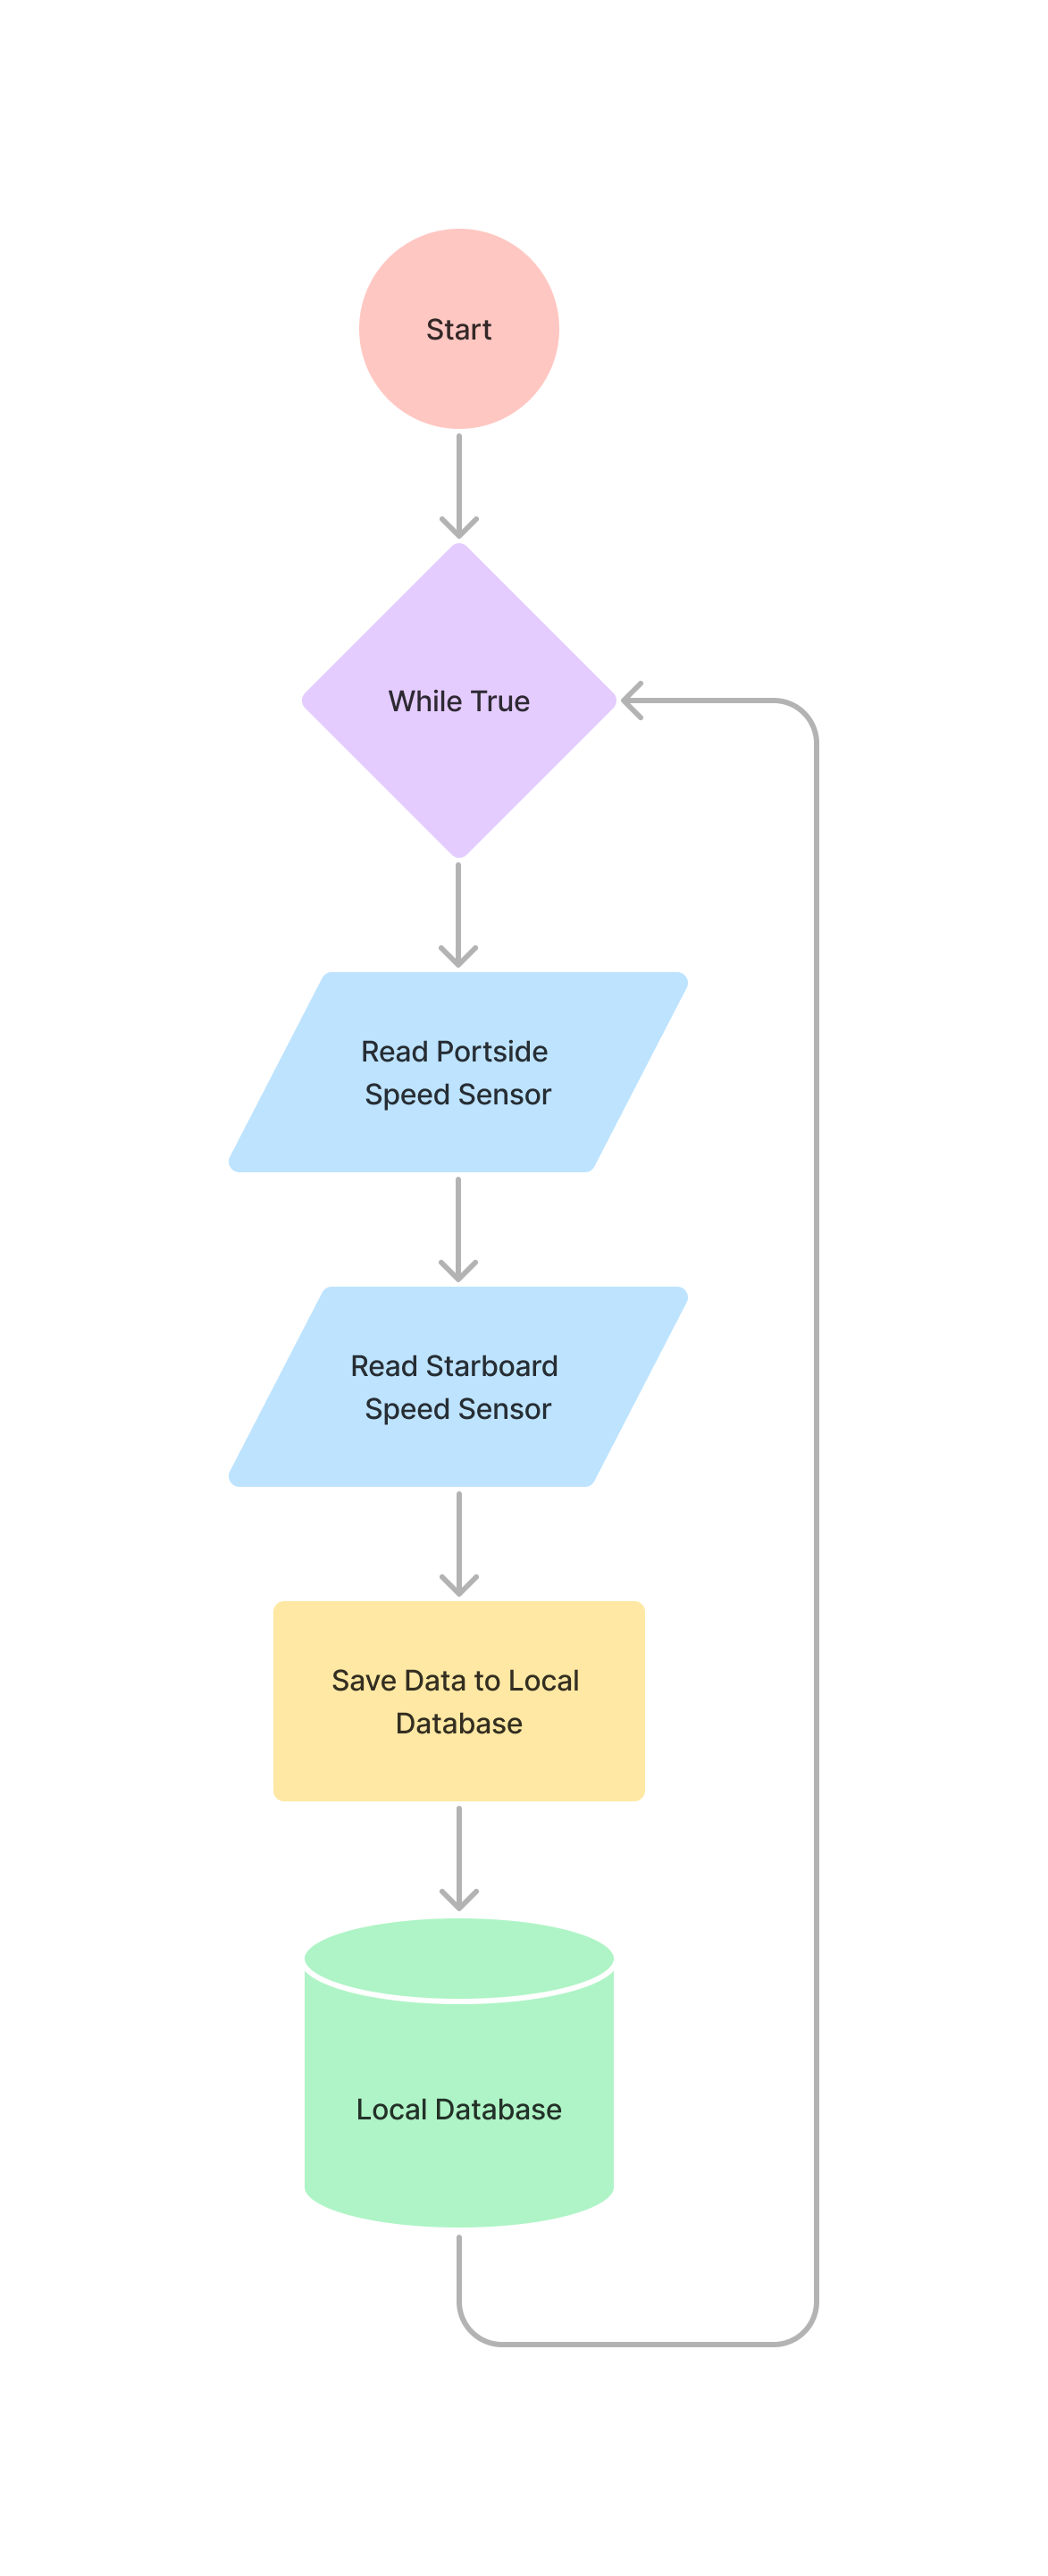
\includegraphics[width=.6\linewidth, center]{images/flowcharts/flow-iot-nodes.png}
%     \caption{Diagram Alir Pengambilan Data Kecepatan Mesin Pada IoT Node}
%     \label{fig:flow-iot-node}
% \end{figure}

% \newpage

% Pada proses sinkronisasi data, \textit{IoT Node} akan mengecek dahulu apakah terdapat koneksi internet saat hendak melakukan pengiriman data. Perlu diingat bahwa ketika kapal beroperasi di wilayah jauh dari daratan, seringkali tidak terdapat koneksi internet. Oleh karenanya, \textit{IoT Node} harus mampu menyimpan data pada penyimpanan internal terlebih dahulu. Untuk menghemat sumber daya komputasi pada Raspberry Pi, proses sinkron selanjutnya akan dilakukan 20 menit kemudian.

% Lebih lanjut, jika terhubung ke internet, \textit{IoT Node} akan mengumpulkan seluruh data yang belum tersinkron, ini ditandai dengan data dengan \textit{sync flag} yang bernilai FALSE. Seluruh data yang akan dikirim akan dikelompokkan menjadi 10 data pada setiap \textit{request}. Jika mendapat respon sukses dari server maka \textit{sync flag} akan diubah menjadi TRUE, dilanjut dengan menampilkan pesan sukses. Sebaliknya, jika mendapat respon error dari server maka \textit{sync flag} akan tetap bernilai FALSE dan akan menampilkan pesan error.

% Berikut merupakan \textit{pseudocode} diagram alir sinkronisasi data pada \textit{IoT Node} yang dapat dilihat pada Tabel \ref{tab:pseudocode-save-to-server} dan Gambar \ref{fig:flow-upload}.

% \begin{longtable}[!h]
  {
          p{0.9\textwidth}
  }
  \caption{Pseudocode Pengiriman Data Ke Server}
  \label{tab:pseudocode-save-to-server} \\

  \hline
      \bfseries Pseudocode \\ [0.5ex]
  \hline

  \endfirsthead

  \hline
      \bfseries Pseudocode \\ [0.5ex]
  \hline
  \endhead % all the lines above this will be repeated on every page

  WHILE TRUE \\
  \hspace{5mm} IF connected to internet THEN \\
  \hspace{10mm} GET unsynchronized engine data \\
  \hspace{10mm} SET data to payload \\
  \hspace{10mm} SEND payload to server with data rate of 10 \\
  \hspace{10mm} RETURN response from server \\
  \hspace{15mm} IF response is success THEN \\
  \hspace{20mm} SET synchronized flag to TRUE \\
  \hspace{20mm} DISPLAY success message \\
  \hspace{15mm} ELSE \\
  \hspace{20mm} DISPLAY error message \\
  \hspace{5mm} ELSE \\
  \hspace{10mm} DISPLAY no internet connection \\
  \hspace{5mm} DELAY 20 minutes \\
  \hspace{5mm} ENDIF \\
  ENDWHILE \\

  \bottomrule
\end{longtable}
% \begin{figure}[!h]
%     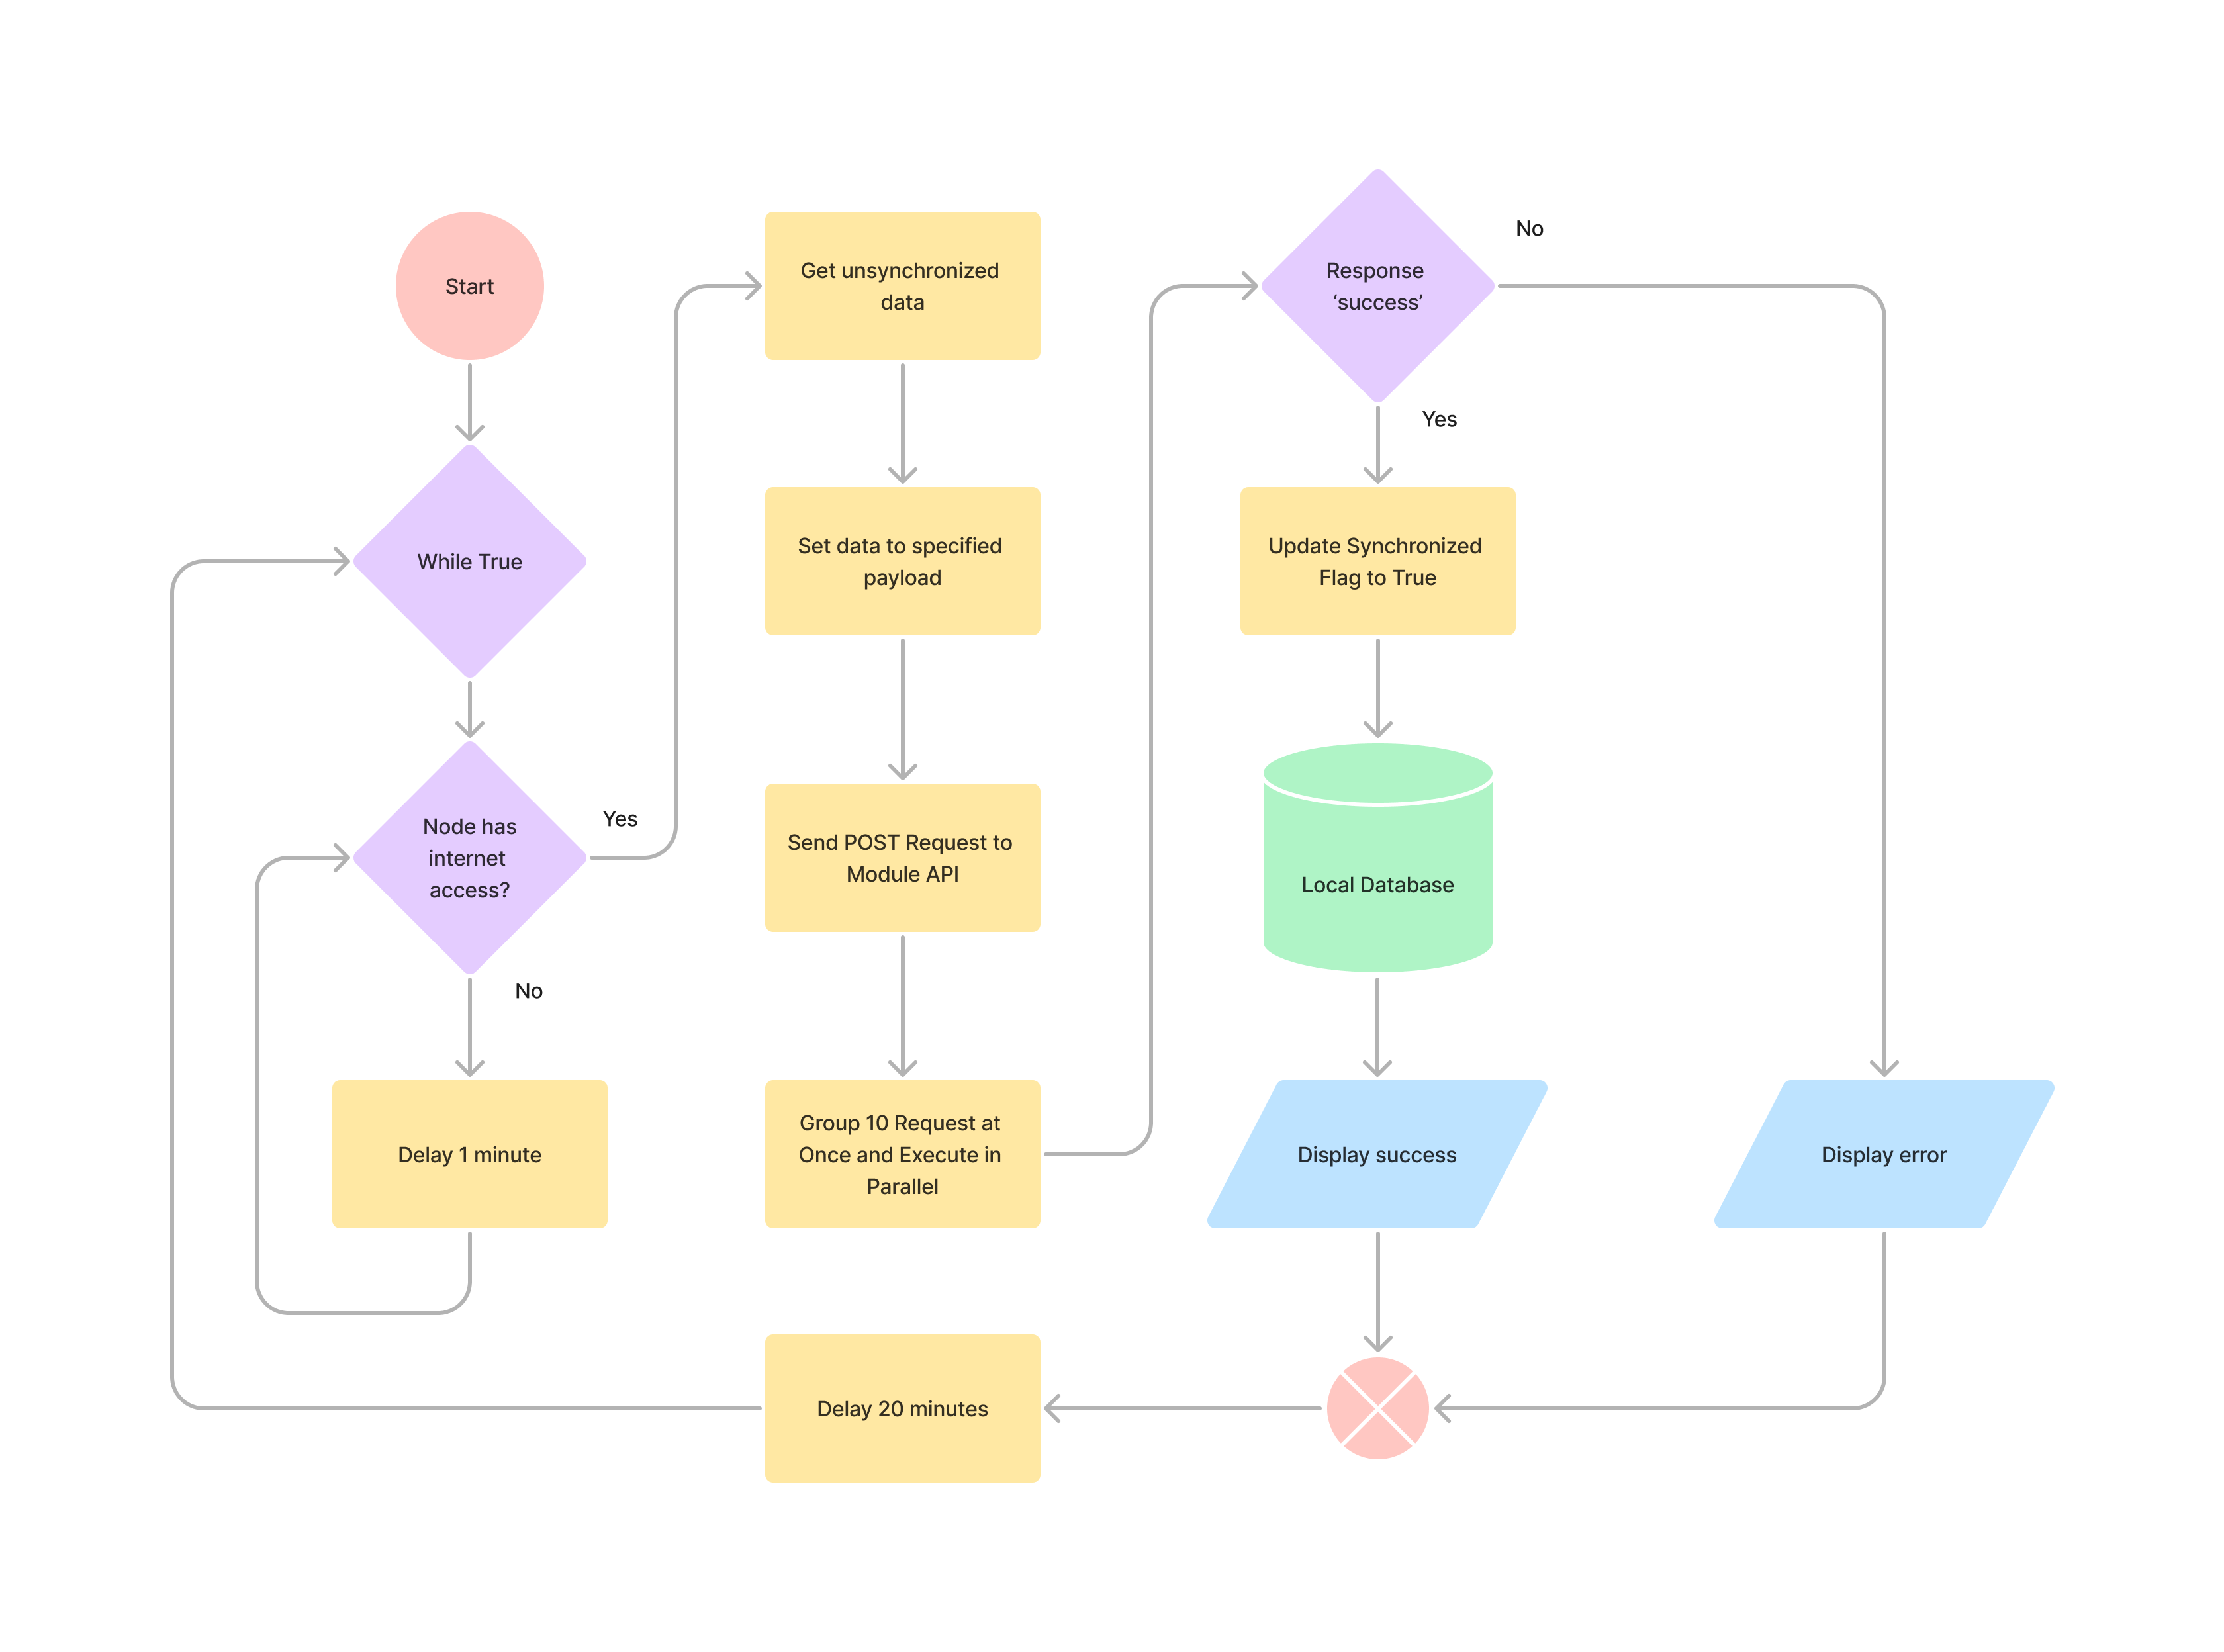
\includegraphics[width=1.2\linewidth, center]{images/flowcharts/flow-save-to-server.png}
%     \caption{Diagram Alir Pengiriman Data Ke Server}
%     \label{fig:flow-upload}
% \end{figure}

\newpage

\subsection{\textit{Whitebox Testing}}

Sebelum diunggah ke \textit{codebase} atau Github, dilakukan pengujian \textit{whitebox} dengan membuat \textit{Unit Test} yang akan dijalankan selama pengembangan. \textit{Unit test} dilakukan pada pengembangan \textit{API} yang merupakan bagian dari \textit{Data Processing Layer} dan \textit{Network Layer}. Hal ini agar data yang akan ditampilkan pada antarmuka sistem merupakan data yang valid sehingga dapat memberikan wawasan yang tepat. Aturan penomoran \textit{whitebox} dapat dilihat pada Tabel \ref{tab:nr-whitebox}.

\begin{table}[!h]
    \caption{Aturan Penomoran Whitebox Testing}
    \centering
    \begin{tabular}
        {
            >{\centering\arraybackslash}p{0.2\textwidth}
            >{\centering\arraybackslash}p{0.4\textwidth}
        }
        \toprule

        Kode &
        Keterangan \\ [1ex]

        \midrule

        SM- & Sistem Monitoring \\
        -WT- & Whitebox Testing \\
        -\{x\}- & Singkatan Nama Fitur \\
        -\{n\} & Nomor Urutan Test Case \\

        \bottomrule
    \end{tabular}
    \label{tab:nr-whitebox}
\end{table}

Hasil perhitungan \textit{cyclomatic complexity (CYC)} pada kode \textit{backend} Engine Speed dimulai dari pembuatan \textit{flowchart} dan \textit{flowgraph} yang dapat dilihat pada Gambar \ref{fig:flow-be-overview} dan Gambar \ref{fig:flowgraph-be-es} secara berturut-turut. Lalu dilakukan perhitungan nilai CYC menggunakan rumus yang sebelumnya telah dijabarkan pada Notasi 2.1.

\begin{figure}[!h]
  \centering
  \tikz[node distance={15mm}, thick, main/.style = {draw, circle}]
  {
      \node[main] (1) {$1$};
      \node[main] (2) [below of=1] {$2$};
      \node[main] (3) [right of=2] {$3$};
      \node[main] (4) [right of=3] {$4$};
      \node[main] (5) [right of=4] {$5$};
      \node[main] (6) [right of=5] {$6$};

      \node[main] (7) [below of=6] {$7$};
      \node[main] (8) [below of=7] {$8$};
      \node[main] (9) [below of=8] {$9$};

      \node[main] (10) [below of=5] {$10$};

      \draw[->] (1) -- (2);
      \draw[->] (2) -- (3);
      \draw[->] (3) -- (4);
      \draw[->] (4) -- (5);
      \draw[->] (5) -- (6);
      \draw[->] (6) -- (7);
      \draw[->] (7) -- (8);
      \draw[->] (8) -- (9);


      \draw[->] (2) to [out=270, in=180, looseness=1] (10);
      \draw[->] (10) to [out=0, in=180, looseness=1] (7);
  }
  \caption{Notasi \textit{Flowgraph Backend} Engine Speed}
  \label{fig:flowgraph-be-es}
\end{figure}

Dari \textit{flowgraph} diatas, terdapat jumlah Node dan Edge masing-masing adalah 10. Berdasarkan rumus perhitungan \ref{eq:cyc}, didapatkan hasil nilai CYC adalah 2. Maka dari itu, telah dibuat 2 \textit{test case} yang dapat dilihat pada Tabel \ref{tab:it1-whitebox-es}.

\begin{equation}\label{eq:cyc-es}
    \begin{split}
        V(G) & = E - N + 2 \\
            & = 10 - 10 + 2 \\
            & = 2
    \end{split}
\end{equation}

Namun, pada praktiknya perhitungan nilai CYC tidak dilakukan secara manual, melainkan menggunakan library Python, yakni \textit{mccabe}. Hasil skor CYC pada kode \textit{backend} dapat dilihat pada Lampiran \ref{apdx:hasil-cc}.

\begin{landscape}
    \begin{longtable}[!h]
    {
            p{0.2\textwidth}
            p{0.3\textwidth}
            p{0.3\textwidth}
            p{0.3\textwidth}
            p{0.2\textwidth}
            p{0.15\textwidth}
    }
    \caption{\textit{Whitebox Testing} API Engine Speed}
    \label{tab:it1-whitebox-es} \\

    \hline
        \bfseries \textit{Test Code} &
        \bfseries \textit{Test Case} &
        \bfseries \textit{Scope} &
        \bfseries \textit{Expected Result} &
        \bfseries \textit{Actual Result} &
        \bfseries \textit{Pass/Fail} \\ [0.5ex]
    \hline

    \endfirsthead

    \hline
        \bfseries \textit{Test Code} &
        \bfseries \textit{Test Case} &
        \bfseries \textit{Scope} &
        \bfseries \textit{Expected Result} &
        \bfseries \textit{Actual Result} &
        \bfseries \textit{Pass/Fail} \\ [0.5ex]
    \hline
    \endhead % all the lines above this will be repeated on every page
    \hline

    \csvreader[
        late after line=\\,
        before reading={\catcode`\#=12},after reading={\catcode`\#=6}
    ]{tables/hasil/iterations/1/whitebox/engine-speed.csv}
    {1=\code, 2=\case, 3=\scope, 4=\expect, 5=\actual, 6=\status}
    {\code & \case & \scope & \expect & \actual & \status} \\

    \bottomrule
\end{longtable}

\end{landscape}



\begin{landscape}

    \subsection{\textit{{Blackbox Testing}}}

    Setelah repositori telah terbarui, mitra dapat langsung mengakses sistem untuk menguji fungsionalitas fitur yang telah dikerjakan pada iterasi tersebut.

    \begin{table}[!h]
    \caption{Aturan Penomoran Blackbox Testing}
    \centering
    \begin{tabular}
        {
            >{\centering\arraybackslash}p{0.2\textwidth}
            >{\centering\arraybackslash}p{0.4\textwidth}
        }
        \toprule

        Kode &
        Keterangan \\ [1ex]

        \midrule

        SM- & Sistem Monitoring \\
        -T- & Testing \\
        -\{x\}- & Singkatan Nama Fitur \\
        -\{n\} & Nomor Urutan Test Case \\

        \bottomrule
    \end{tabular}
    \label{tab:nr-blackbox}
\end{table}

    \textit{Test case} yang dibuat untuk Halaman Engine Speed memastikan grafik telah ditampilkan dengan sesuai dan ketika pengguna melakukan filter tanggal, data grafik akan terubah sesuai dengan data tanggal yang diinput. Berikut hasil \textit{test case} untuk iterasi 1

    \begin{longtable}[!h]
    {
            p{0.2\textwidth}
            p{0.3\textwidth}
            p{0.3\textwidth}
            p{0.3\textwidth}
            p{0.3\textwidth}
            p{0.15\textwidth}
    }
    \caption{\textit{Blackbox Testing} Halaman Engine Speed}
    \label{tab:it1-blackbox-es} \\

    \hline
        \bfseries \textit{Test Code} &
        \bfseries \textit{Test Case} &
        \bfseries \textit{Test Steps} &
        \bfseries \textit{Expected Result} &
        \bfseries \textit{Actual Result} &
        \bfseries \textit{Pass/Fail} \\ [0.5ex]
    \hline

    \endfirsthead

    \hline
        \bfseries \textit{Test Code} &
        \bfseries \textit{Test Case} &
        \bfseries \textit{Test Steps} &
        \bfseries \textit{Expected Result} &
        \bfseries \textit{Actual Result} &
        \bfseries \textit{Pass/Fail} \\ [0.5ex]
    \hline
    \endhead % all the lines above this will be repeated on every page
    \hline

    \csvreader[
        late after line=\\,
        before reading={\catcode`\#=12},after reading={\catcode`\#=6}
    ]{tables/hasil/iterations/1/blackbox/engine-speed.csv}
    {1=\code, 2=\case, 3=\step, 4=\expect, 5=\actual, 6=\status}
    {\code & \case & \step & \expect & \actual & \status} \\

    \bottomrule
\end{longtable}
\end{landscape}

\section{\textit{Productionizing Phase}}

Selama pengerjaan berlangsung, terdapat beberapa umpan balik dari mitra yang mengakibatkan penambahan pada \textit{task}. Sehingga, ini juga berdampak pada rencana iterasi yang sebelumnya telah dibuat. Secara garis besar, \textit{task} yang bertambah adalah sistem admin untuk melakukan manajemen data kapal, manajemen data pengguna, manajemen data FCRV dan beberapa halaman tambahan untuk pengguna. Hasil akhir, umpan balik dapat dilihat pada Tabel \ref{tab:feedback}

\begin{longtable}[!h]
    {
            p{0.15\textwidth}
            p{0.4\textwidth}
            p{0.2\textwidth}
            p{0.2\textwidth}
    }
    \caption{Umpan Balik Selama Pengembangan}
    \label{tab:feedback} \\

    \hline
        \bfseries No &
        \bfseries Umpan Balik &
        \bfseries Iterasi &
        \bfseries Status \\ [0.5ex]
    \hline

    \endfirsthead

    \hline
        \bfseries No &
        \bfseries Umpan Balik &
        \bfseries Iterasi &
        \bfseries Status \\ [0.5ex]
    \hline
    \endhead % all the lines above this will be repeated on every page
    \hline

    \csvreader[
        late after line=\\,
        before reading={\catcode`\#=12},after reading={\catcode`\#=6}
    ]{tables/hasil/changes.csv}{1=\no, 2=\feedback, 3=\i, 4=\status}{\no & \feedback & \i & \status} \\

    \bottomrule
\end{longtable}

Pada iterasi kedua, terdapat permintaan untuk mencantumkan angka \textit{running hour} pada Halaman Engine Speed yang diposisikan dibawah angka kecepatan mesin. Lalu pada iterasi 3 terdapat permintaan tambahan untuk membangun sistem admin agar mitra dapat lebih leluasa untuk melakukan konfigurasi data. Sistem admin meliputi manajemen data pengguna, data kapal, dan data FCRV. Setelah direkap di \textit{user story} dan dilakukan skala prioritas, pengembagan Sistem Admin akan dilakukan pada iterasi 3. Pada iterasi 4, ditambakan halaman Overview yang berisi data kecepatan mesin terakhir dan data ringkasan konsumsi bahan bakar yang dapat dilihat pada gambar \ref{fig:fe-overview}. Terakhir, pada iterasi 5 terdapat permintaan untuk menambah 2 halaman, yakni Home dan OP41 Report. Halaman Home berisi seluruh kapal yang terdaftar dan Halaman OP41 Report berisi laporan konsumsi bahan bakar berdasarkan perhitungan dari kategori FCRV yang dapat dilihat pada Gambar \ref{fig:fe-home} dan Gambar \ref{fig:fe-op41}.

\begin{figure}[!h]
    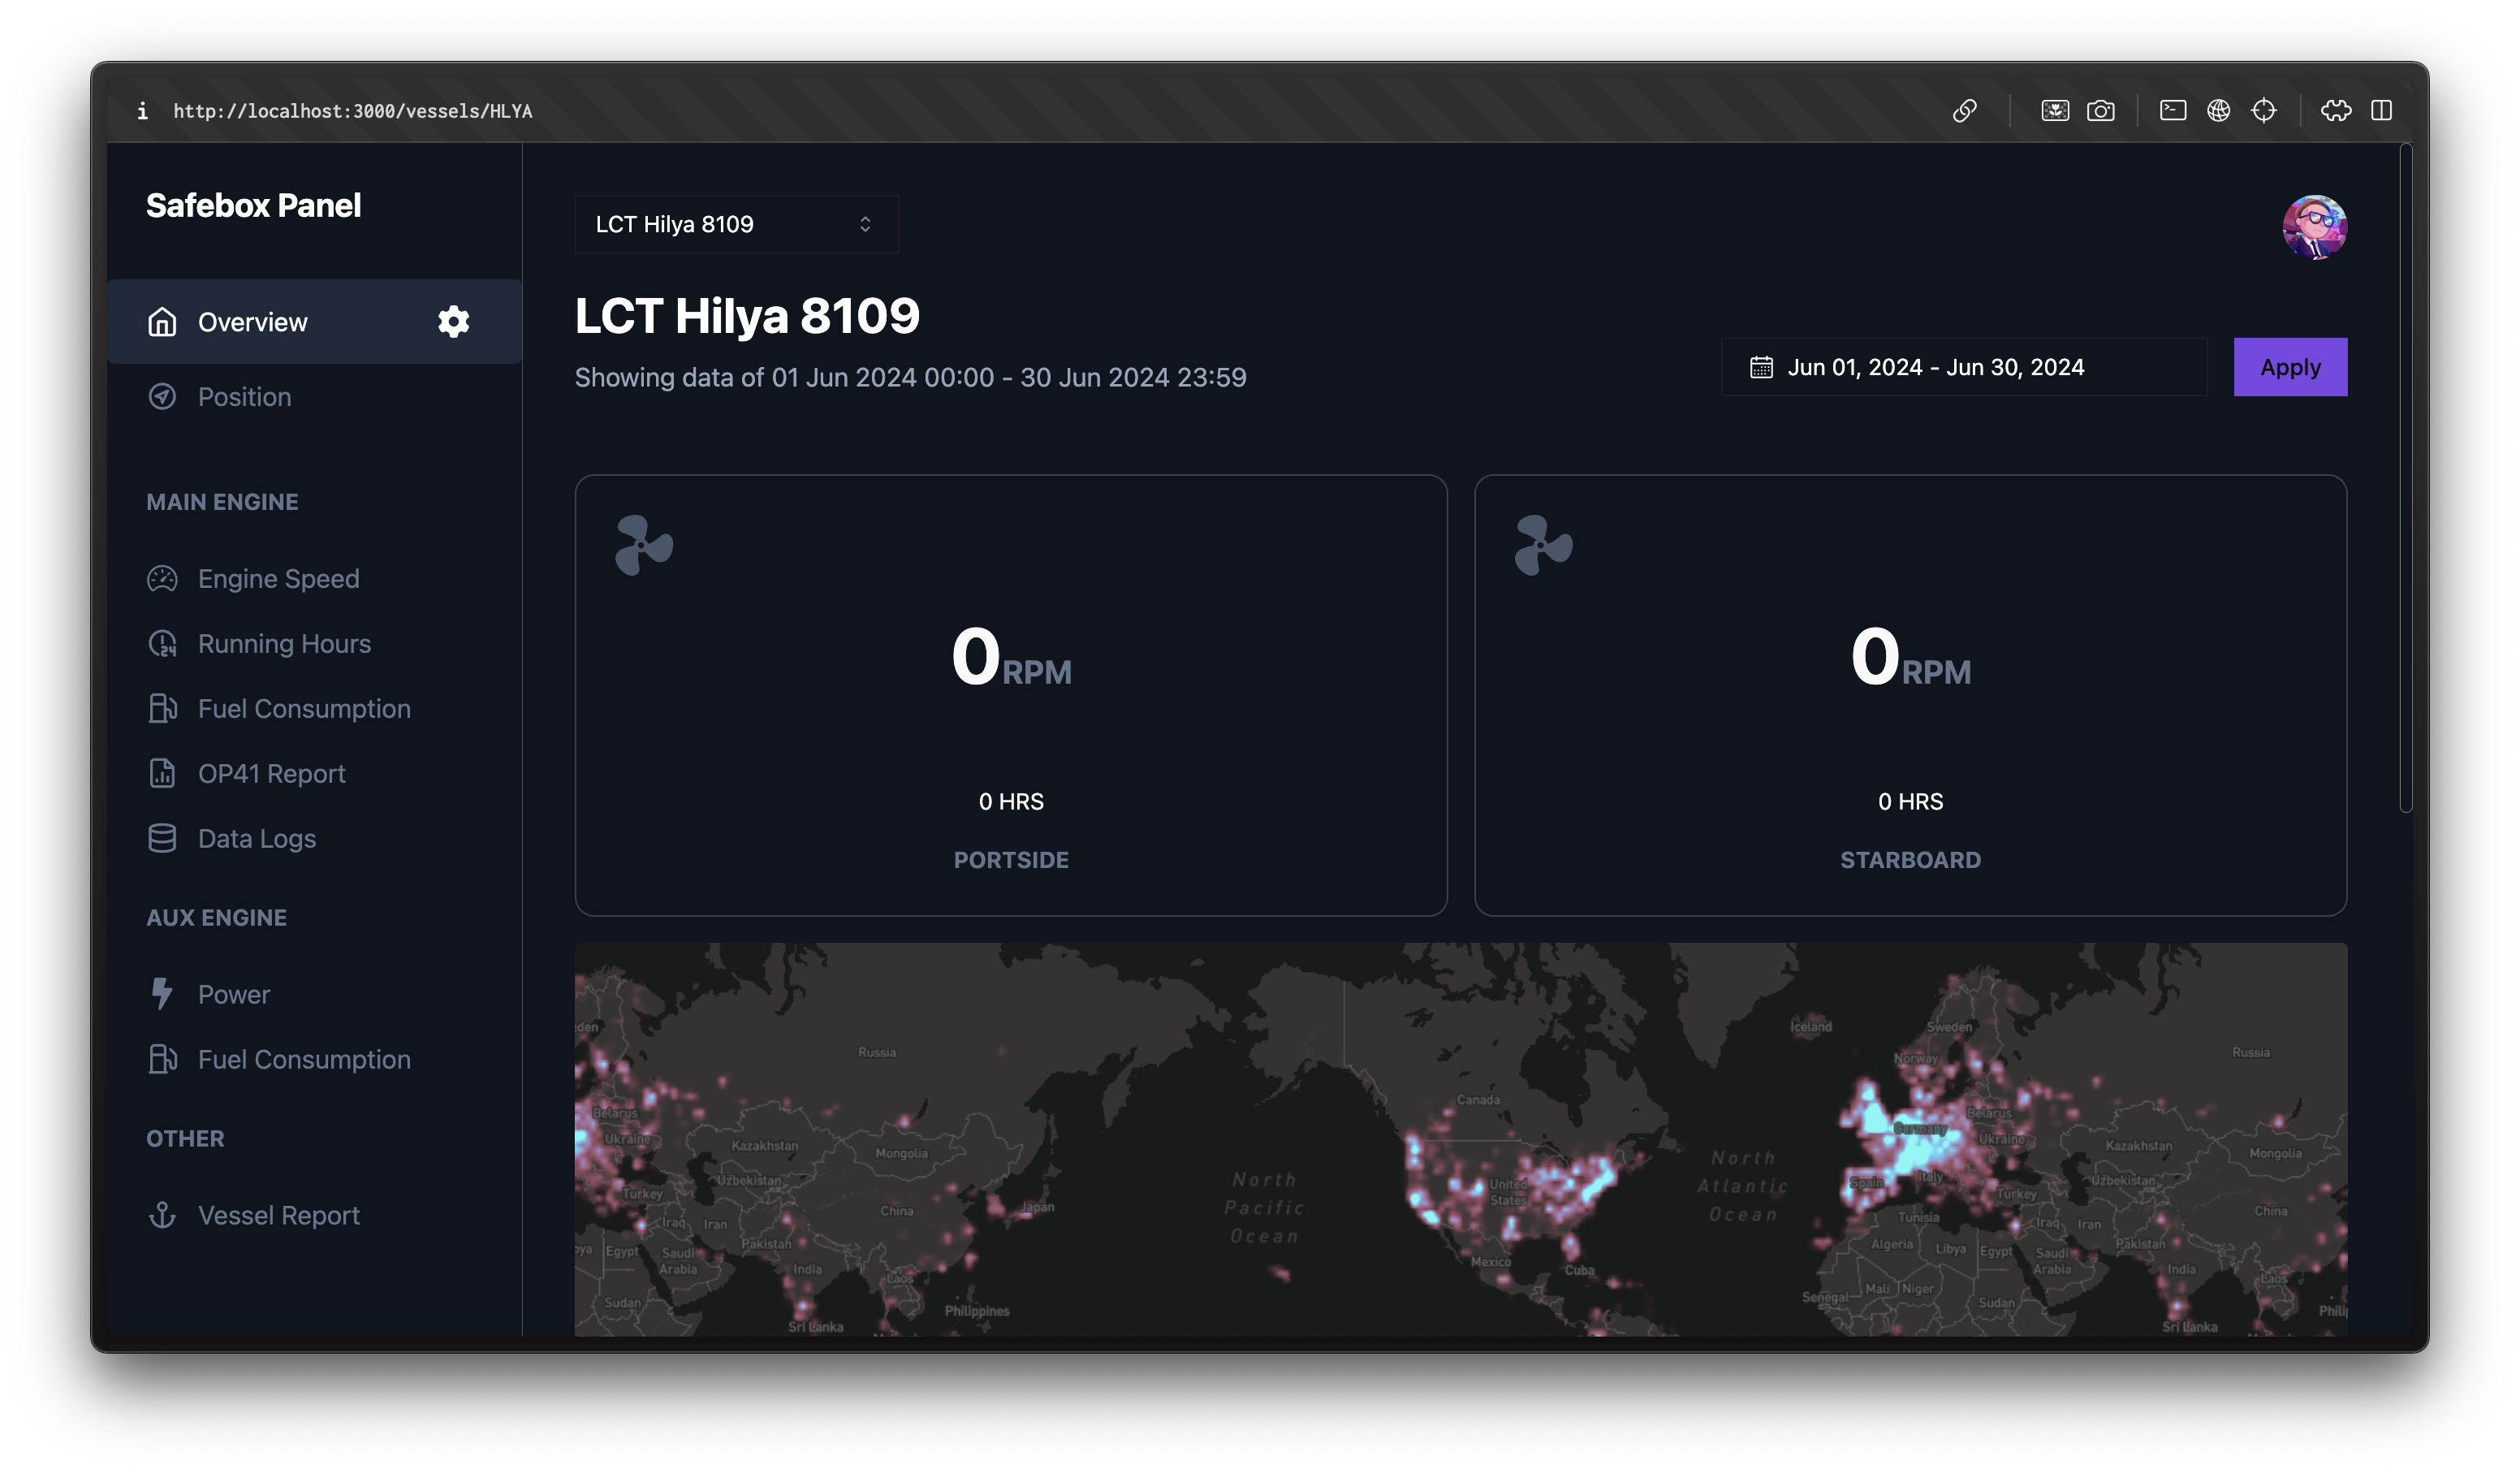
\includegraphics[width=1.05\linewidth, center]{images/hasil/iterations/4/fe-overview.png}
    \caption{Frontend Halaman Overview}
    \label{fig:fe-overview}
\end{figure}

\begin{figure}[!h]
    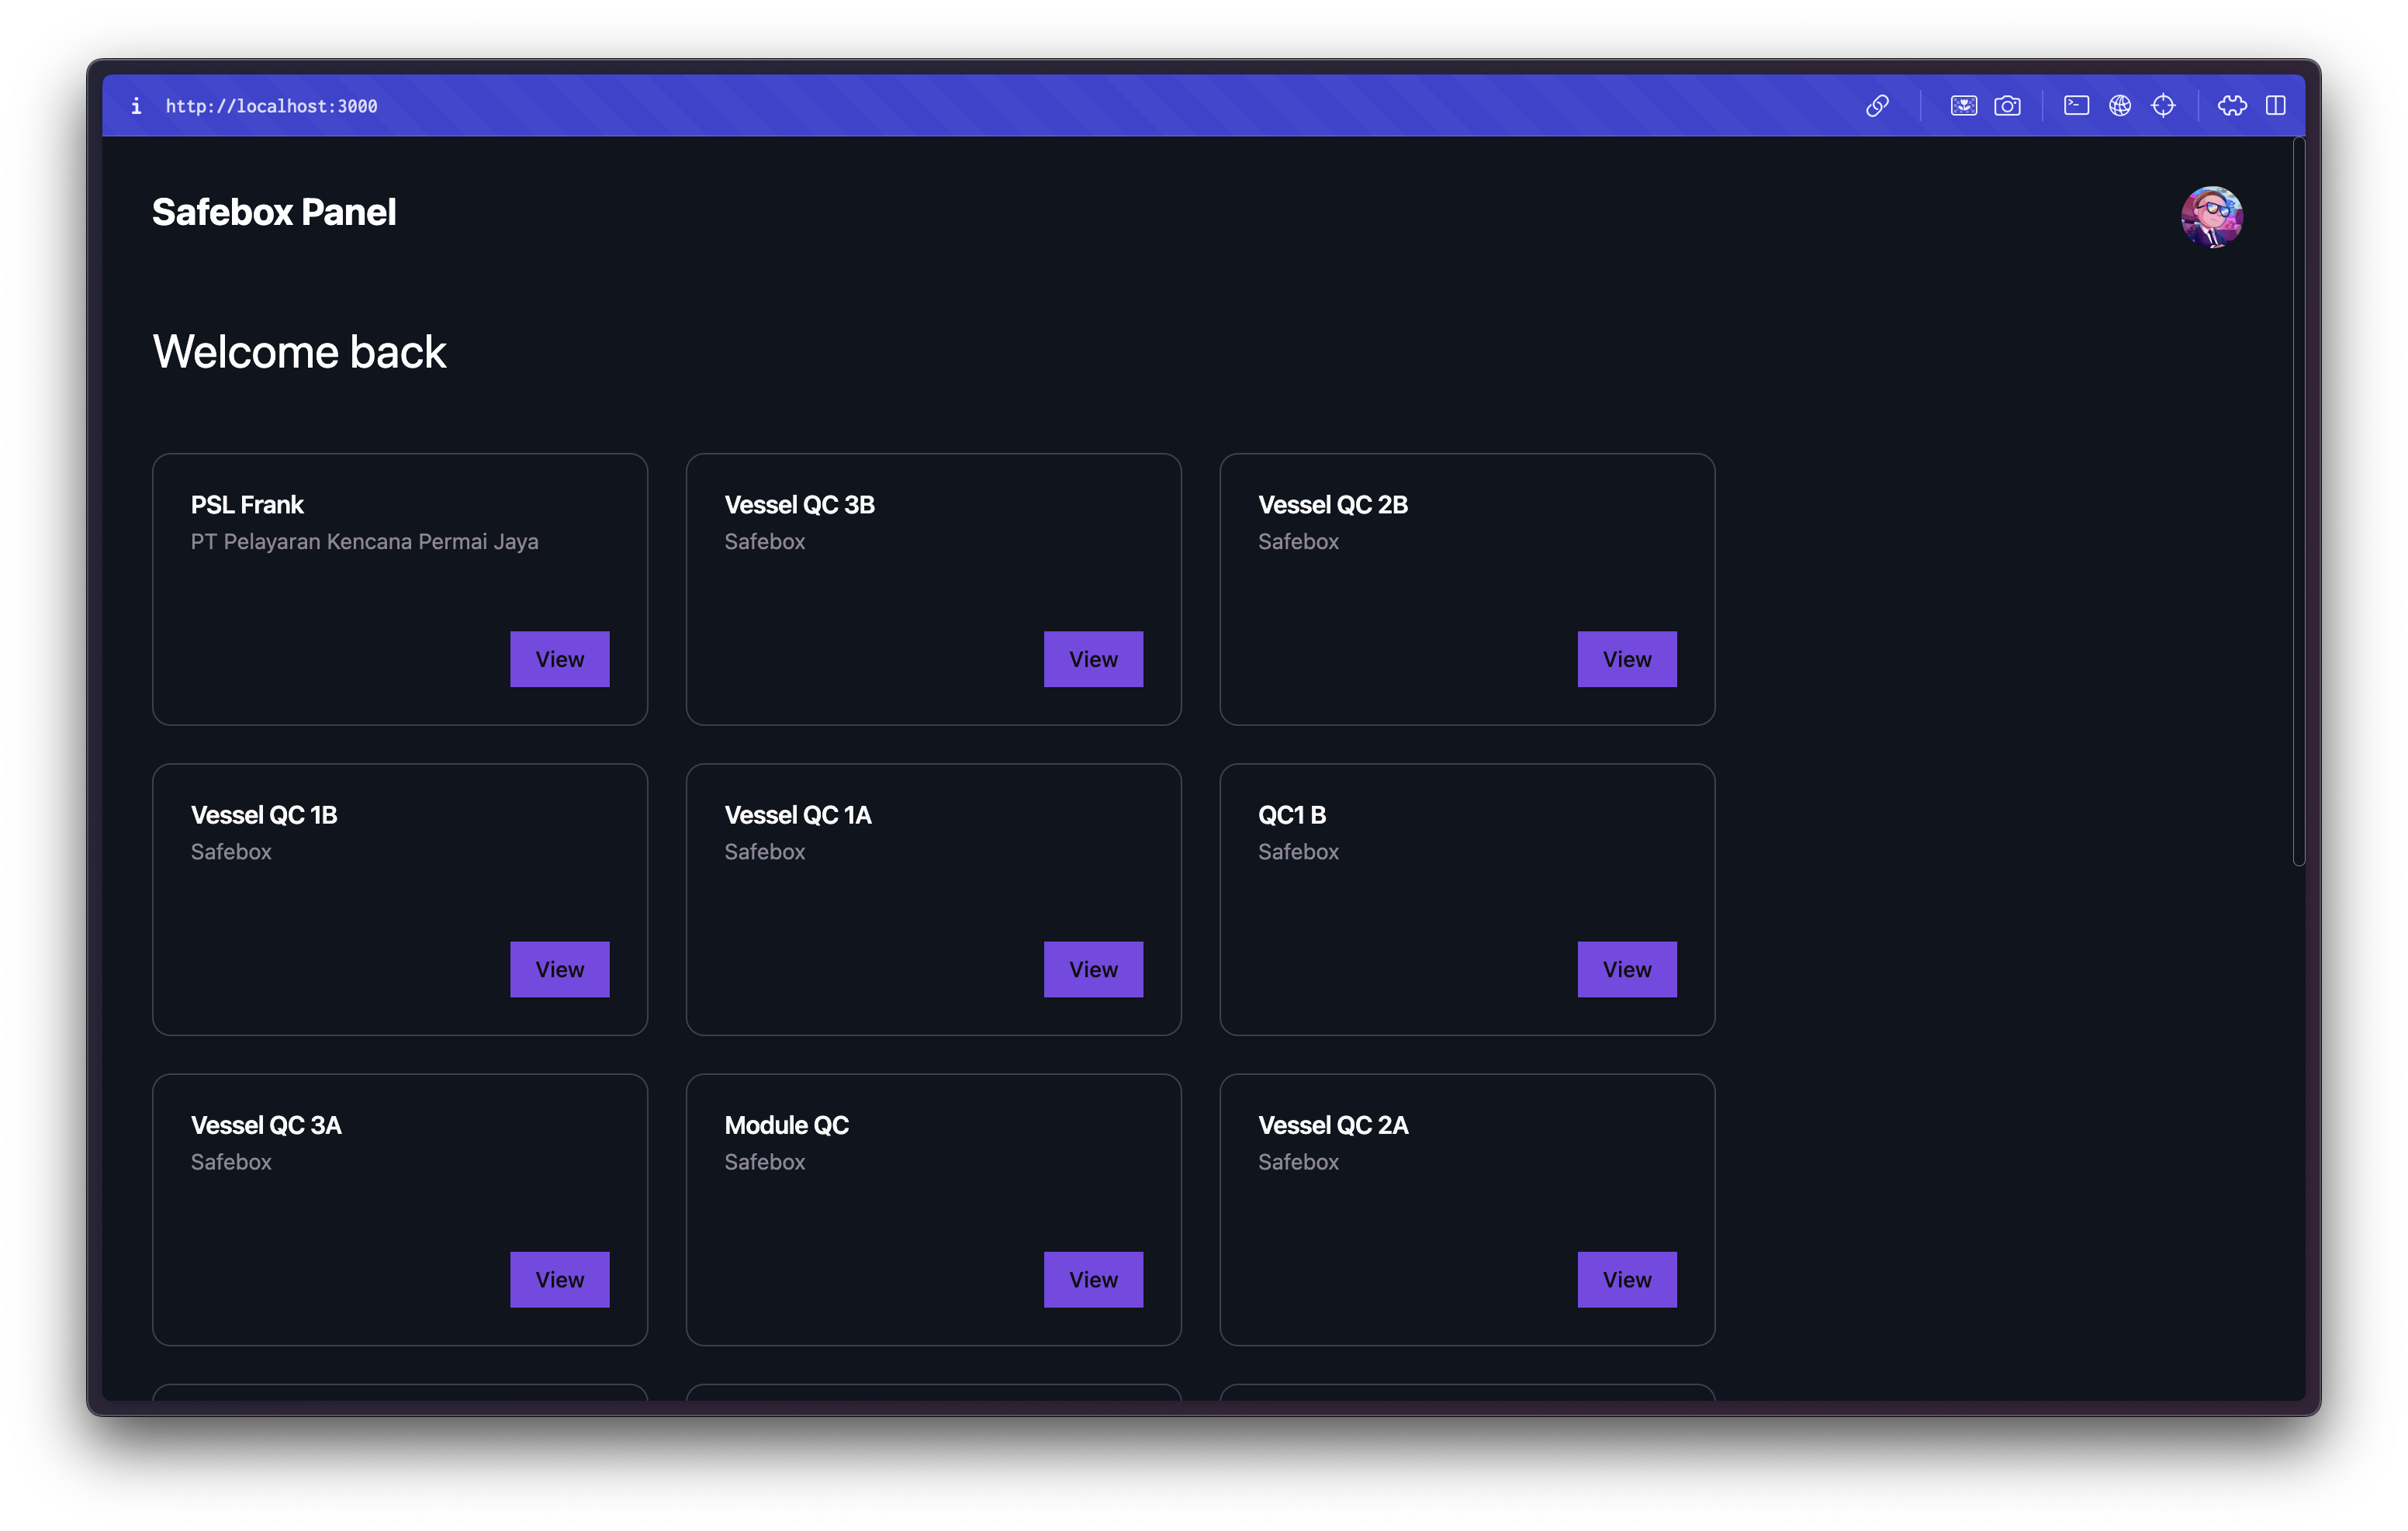
\includegraphics[width=1.05\linewidth, center]{images/hasil/iterations/5/fe-home.png}
    \caption{Frontend Halaman Home}
    \label{fig:fe-home}
\end{figure}

\begin{figure}[!h]
    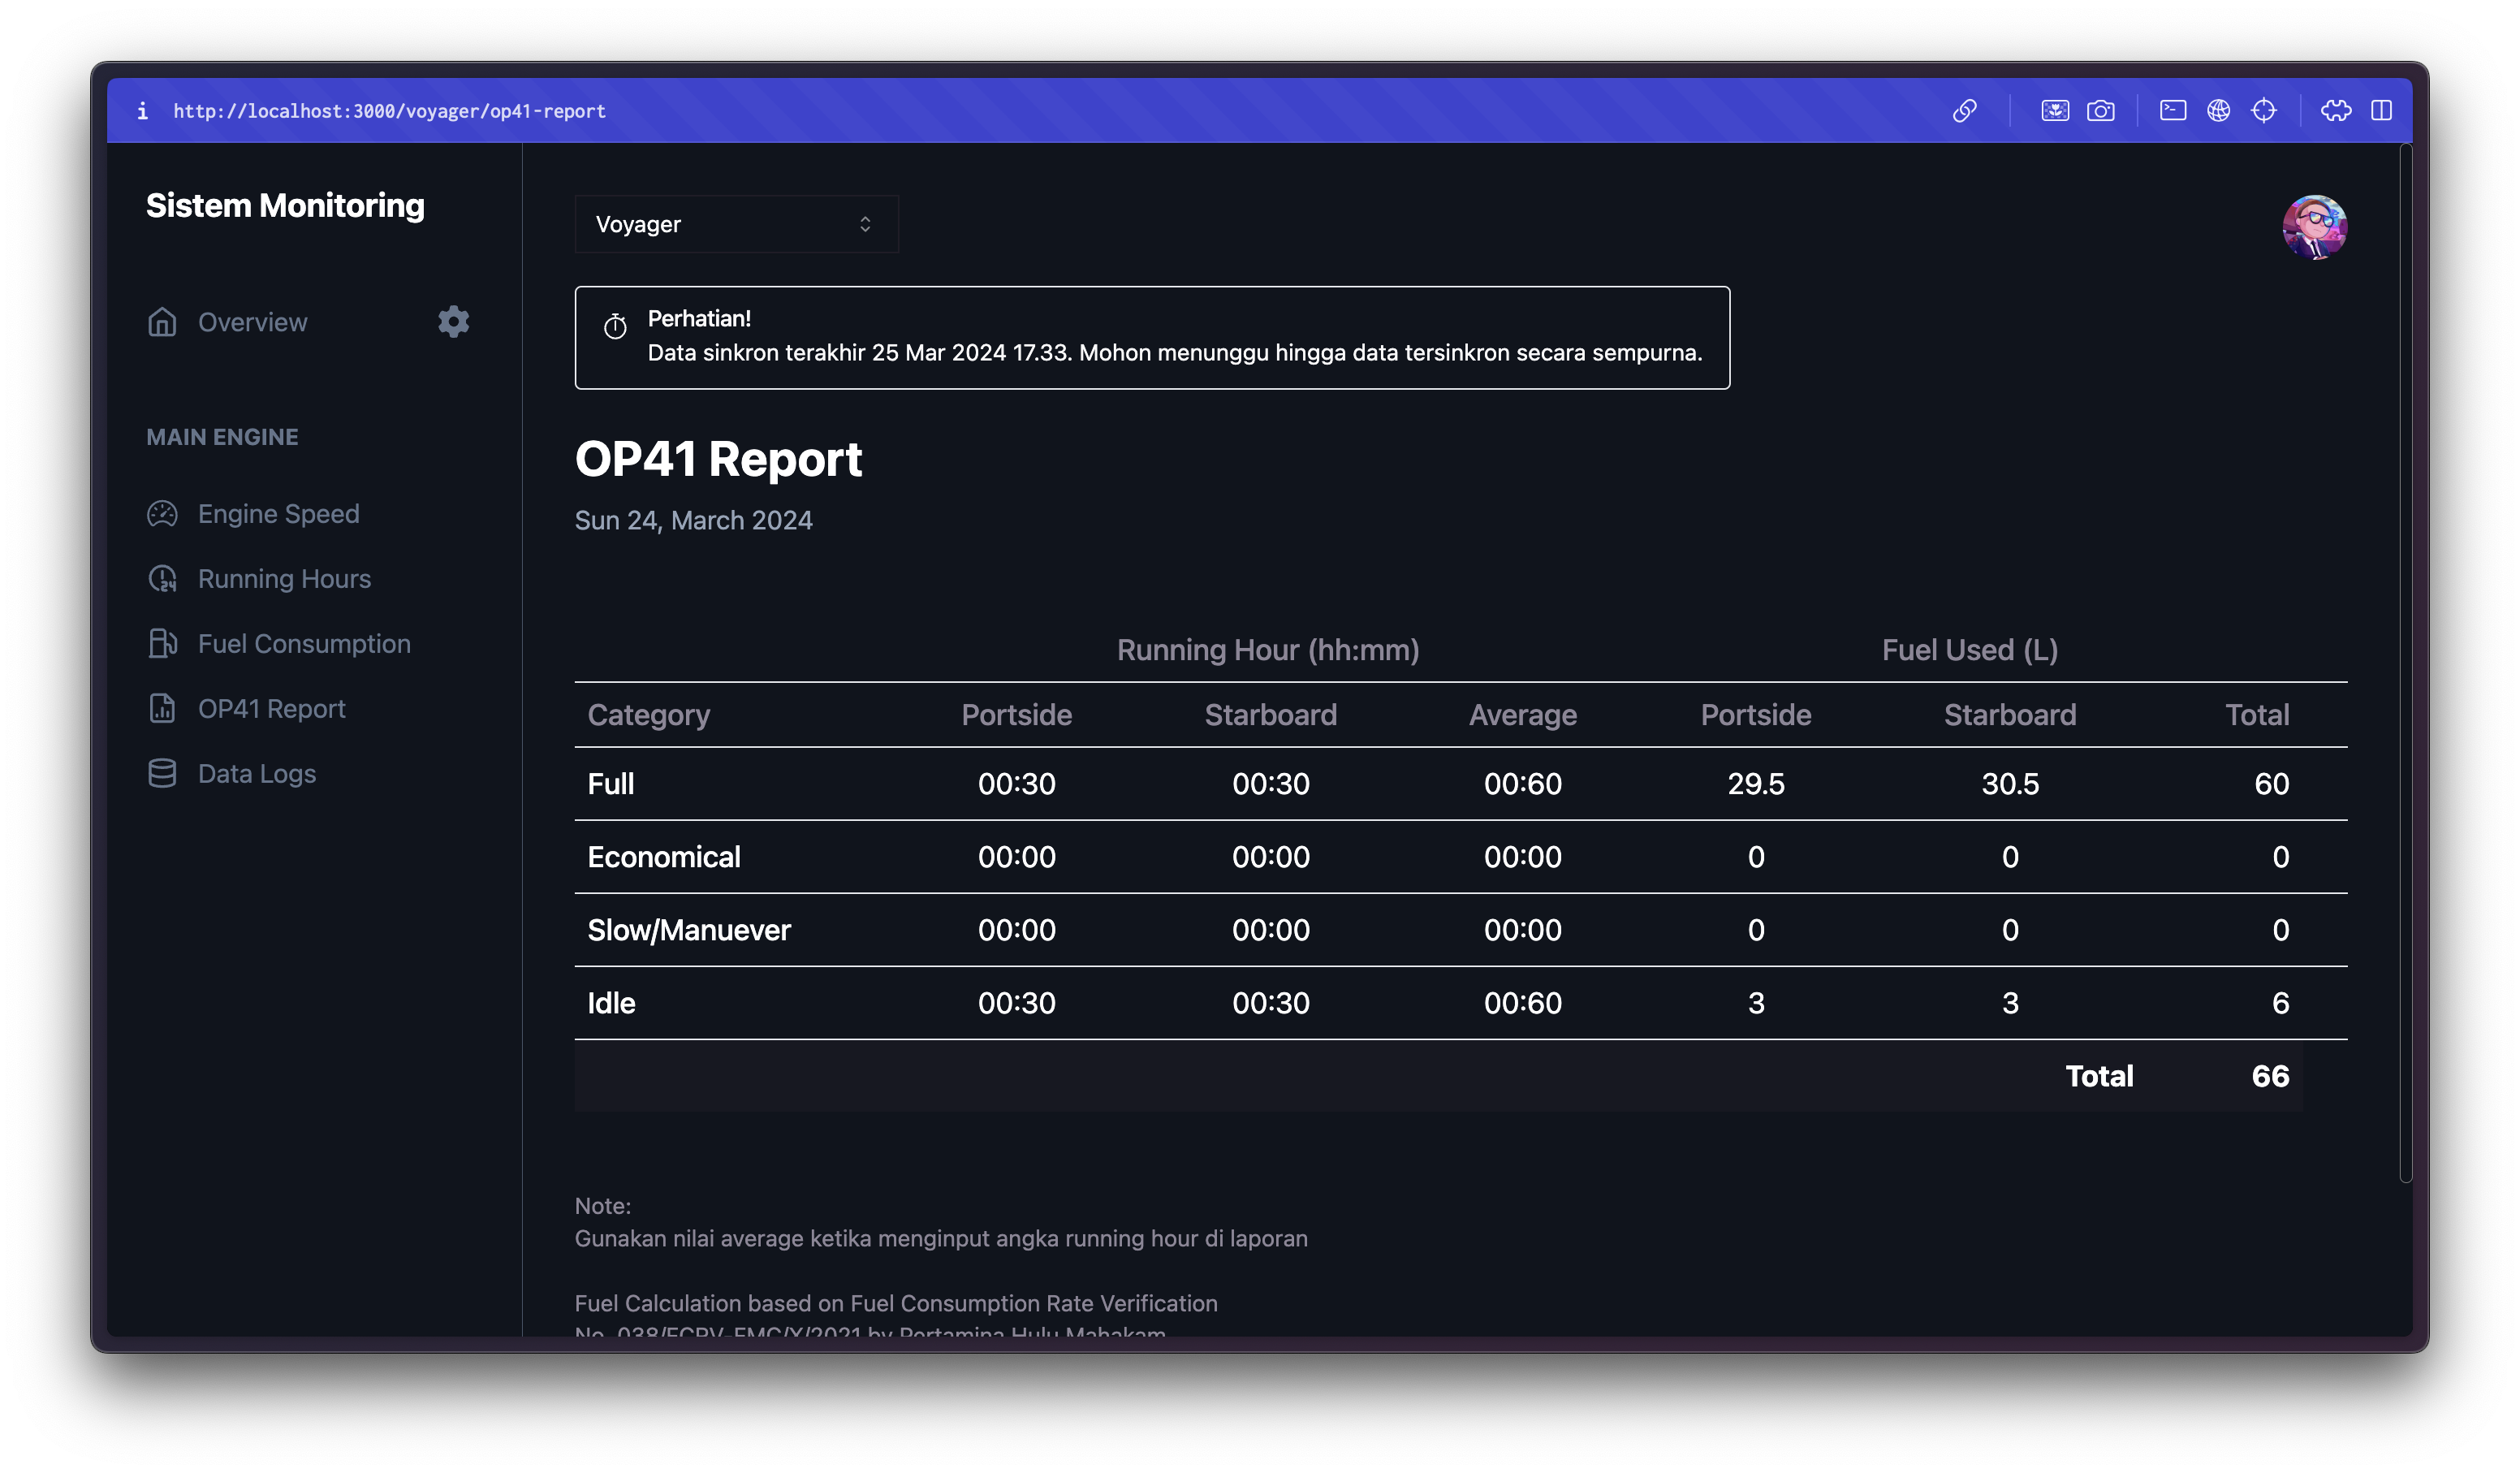
\includegraphics[width=1.05\linewidth, center]{images/hasil/iterations/5/fe-op41.png}
    \caption{Frontend Halaman OP41 Report}
    \label{fig:fe-op41}
\end{figure}

\section{\textit{Maintenance Phase}}

Pada fase ini, Sistem Monitoring sudah dapat digunakan layaknya produk akhir. Seluruh data yang diinput pada Sistem merupakan data asli yang telah terhubung dengan basis data utama. Fase ini diakhiri dengan penandada tanganan Dokumen User Acceptance Test (UAT) oleh mitra yang dapat dilihat pada Lampiran \ref{apdx:hasil}.

\section{\textit{Death Phase}}

Pada akhirnya, konfigurasi lingkungan diubah dari \textit{'development'} menjadi \textit{'production'}. Hasil akhir dari fase ini adalah sebuah sistem yang siap untuk digunakan oleh pengguna.






% Backup >?

% \begin{figure}[!h]
%     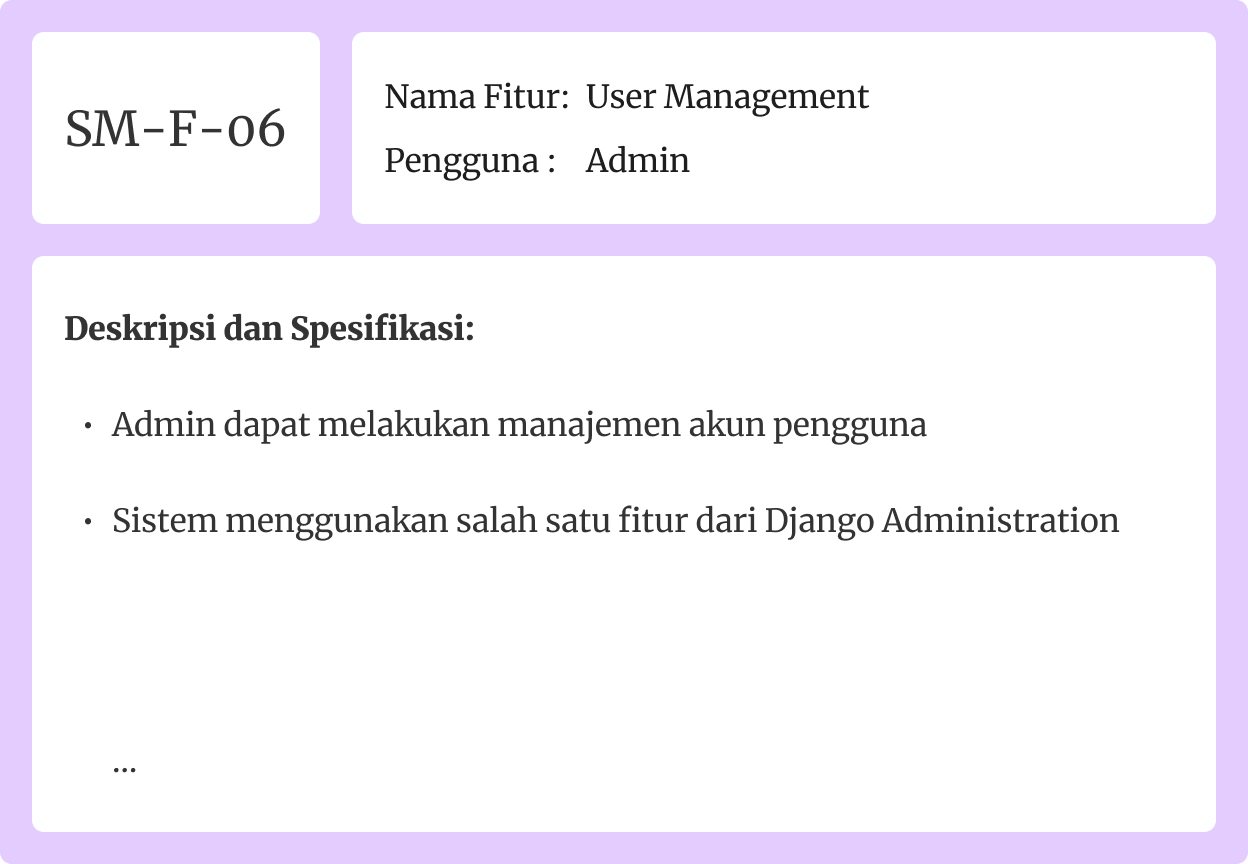
\includegraphics[width=.8\linewidth, center]{images/hasil/iterations/3/fr-user.png}
%     \caption{Kebutuhan Fungsional User Management}
%     \label{fig:fr-user}
% \end{figure}
% \begin{figure}[!h]
%     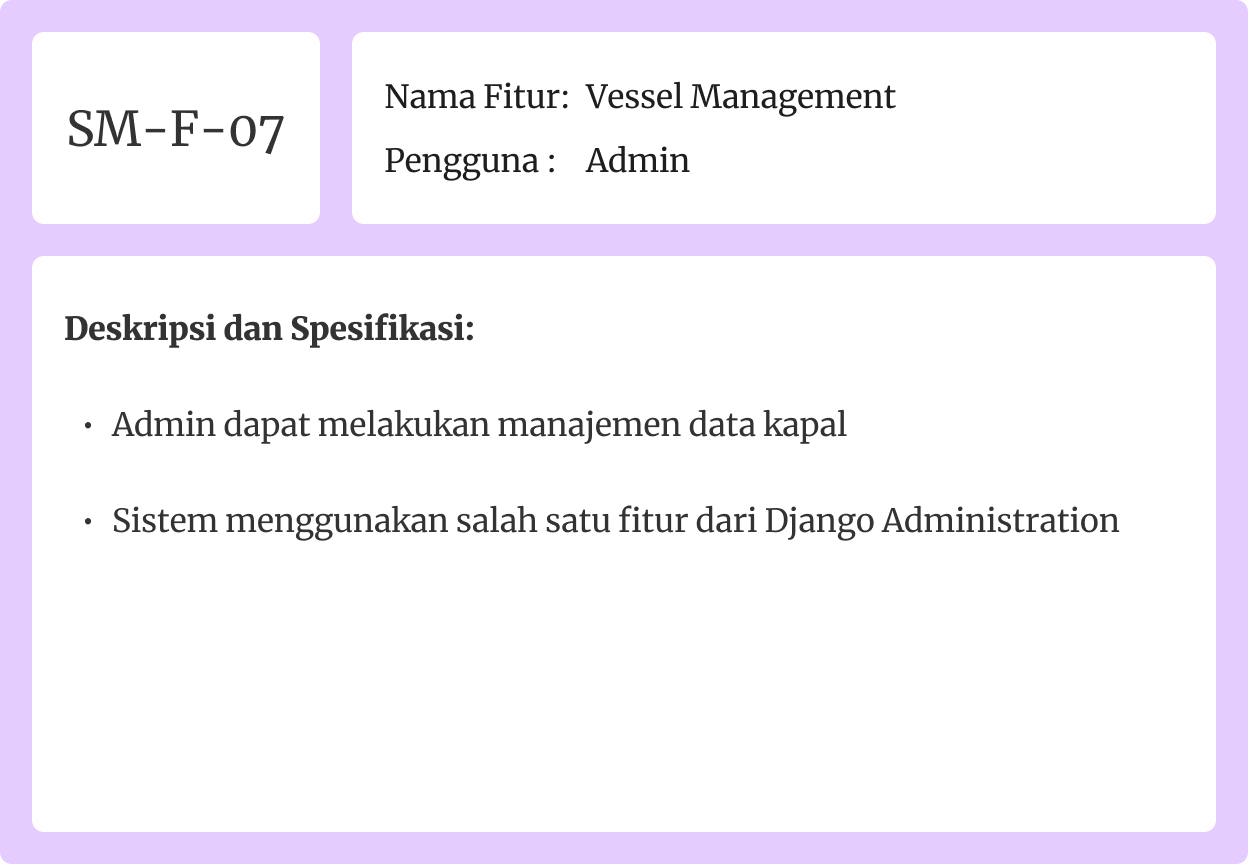
\includegraphics[width=.8\linewidth, center]{images/hasil/iterations/3/fr-vessel.png}
%     \caption{Kebutuhan Fungsional Vessel Management}
%     \label{fig:fr-vessel}
% \end{figure}
% \begin{figure}[!h]
%     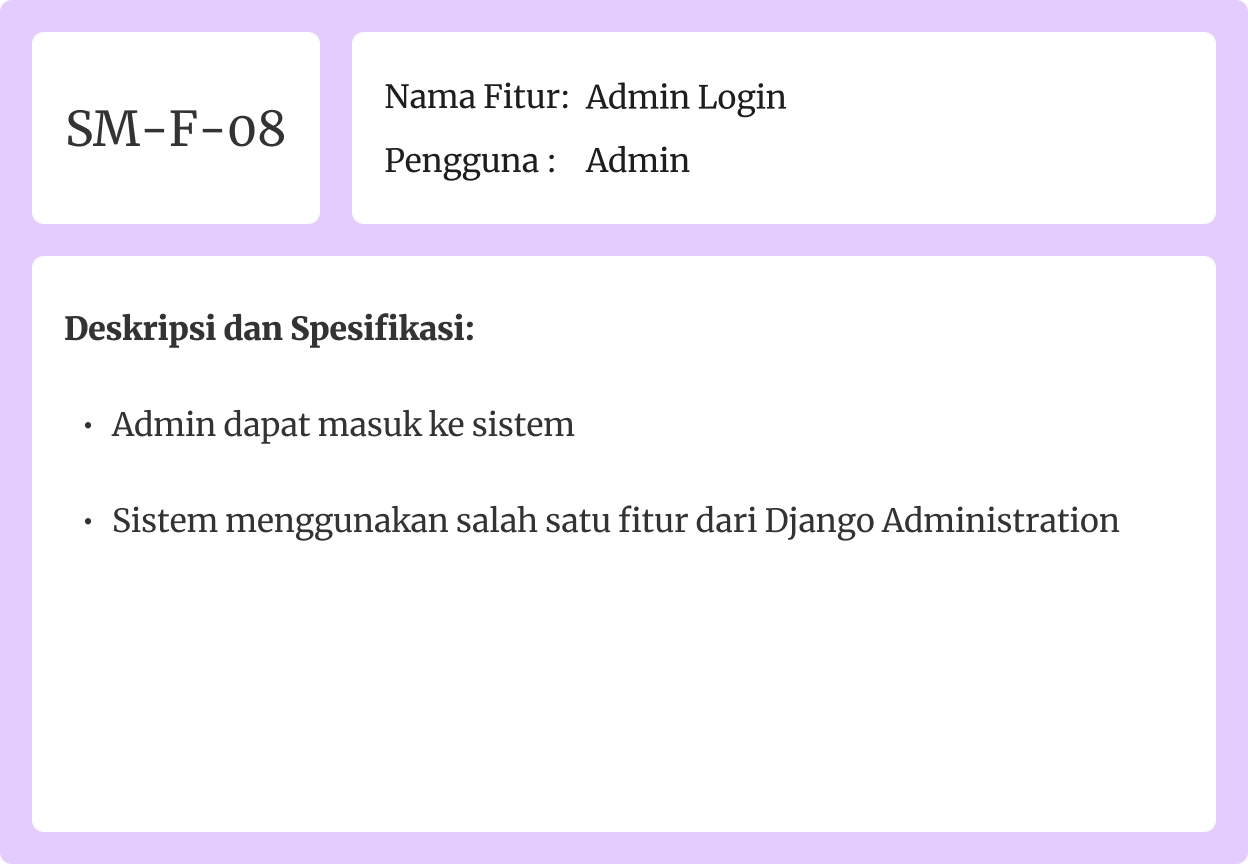
\includegraphics[width=.8\linewidth, center]{images/hasil/iterations/3/fr-login.png}
%     \caption{Kebutuhan Fungsional Admin Login}
%     \label{fig:fr-login-admin}
% \end{figure}

% \begin{figure}[!h]
%     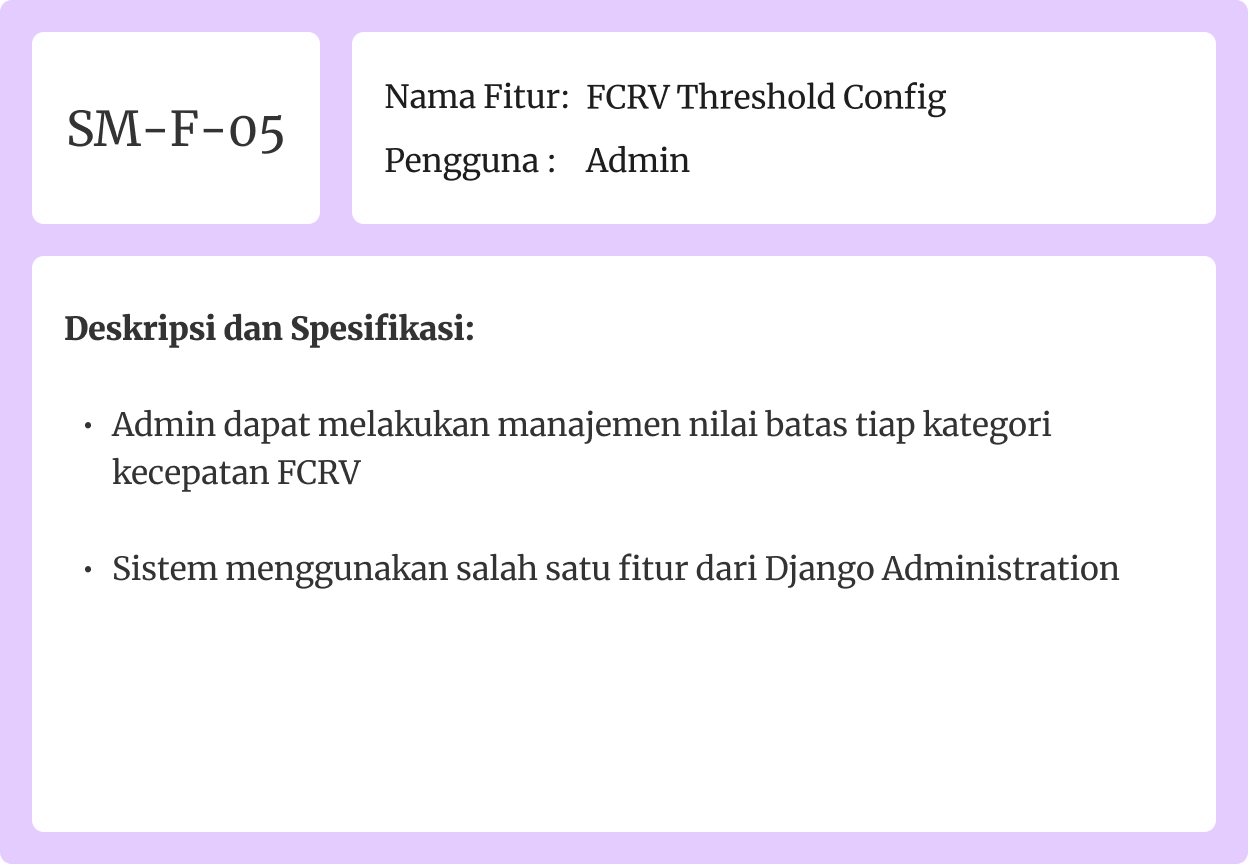
\includegraphics[width=.8\linewidth, center]{images/hasil/iterations/3/fr-fcrv.png}
%     \caption{Kebutuhan Fungsional Admin Logout}
%     \label{fig:fr-logout-admin}
% \end{figure}

% \newpage

% \subsubsection{Desain}

% Pada Sistem Admin, tidak dilakukan desain wireframe dikarenakan fitur bawaan framewok Django yang telah menyediakan Sistem Admin secara otomatis bernama Django administration.

% \subsubsection{Coding}

% Halaman Admin memungkinkan pengguna untuk melakukan operasi CRUD (create, read, update, dan delete) pada data pengguna, kapal, dan FCRV threshold. Hasil halaman yang dibuat oleh Django administration dapat dilihat pada Gambar ... hingga Gambar ... .

% \subsubsection{Whitebox Testing}

% Pada Django administration, seluruh komponen web dihasilkan oleh library bawaan dari package restapi yang telah diabstraksi sedemikian rupa dan telah memiliki alur pengujian sendiri. Sehingga, tidak dimungkinkan untuk dilakukan pengujian melalui unit test yang dibuat sendiri.

% \begin{landscape}
%     \subsubsection{Blackbox Testing}

%     \begin{longtable}[!h]
    {
            p{0.2\textwidth}
            p{0.3\textwidth}
            p{0.3\textwidth}
            p{0.3\textwidth}
            p{0.3\textwidth}
            p{0.15\textwidth}
    }
    \caption{Blackbox Testing Halaman User Management}
    \label{tab:it2-blackbox-user} \\

    \hline
        \bfseries \textit{Test Code} &
        \bfseries \textit{Test Case} &
        \bfseries \textit{Test Steps} &
        \bfseries \textit{Expected Result} &
        \bfseries \textit{Actual Result} &
        \bfseries \textit{Pass/Fail} \\ [0.5ex]
    \hline

    \endfirsthead

    \hline
        \bfseries \textit{Test Code} &
        \bfseries \textit{Test Case} &
        \bfseries \textit{Test Steps} &
        \bfseries \textit{Expected Result} &
        \bfseries \textit{Actual Result} &
        \bfseries \textit{Pass/Fail} \\ [0.5ex]
    \hline
    \endhead % all the lines above this will be repeated on every page
    \hline

    \csvreader[
        late after line=\\,
        before reading={\catcode`\#=12},after reading={\catcode`\#=6}
    ]{tables/hasil/iterations/3/blackbox/user.csv}
    {1=\code, 2=\case, 3=\step, 4=\expect, 5=\actual, 6=\status}
    {\code & \case & \step & \expect & \actual & \status} \\

    \bottomrule
\end{longtable}
%     \newpage
%     \begin{longtable}[!h]
    {
            p{0.2\textwidth}
            p{0.3\textwidth}
            p{0.3\textwidth}
            p{0.3\textwidth}
            p{0.3\textwidth}
            p{0.15\textwidth}
    }
    \caption{Blackbox Testing Halaman Vessel Management}
    \label{tab:it3-blackbox-vessel} \\

    \hline
        \bfseries \textit{Test Code} &
        \bfseries \textit{Test Case} &
        \bfseries \textit{Test Steps} &
        \bfseries \textit{Expected Result} &
        \bfseries \textit{Actual Result} &
        \bfseries \textit{Pass/Fail} \\ [0.5ex]
    \hline

    \endfirsthead

    \hline
        \bfseries \textit{Test Code} &
        \bfseries \textit{Test Case} &
        \bfseries \textit{Test Steps} &
        \bfseries \textit{Expected Result} &
        \bfseries \textit{Actual Result} &
        \bfseries \textit{Pass/Fail} \\ [0.5ex]
    \hline
    \endhead % all the lines above this will be repeated on every page
    \hline

    \csvreader[
        late after line=\\,
        before reading={\catcode`\#=12},after reading={\catcode`\#=6}
    ]{tables/hasil/iterations/3/blackbox/vessel.csv}
    {1=\code, 2=\case, 3=\step, 4=\expect, 5=\actual, 6=\status}
    {\code & \case & \step & \expect & \actual & \status} \\

    \bottomrule
\end{longtable}
%     \newpage
%     \begin{longtable}[!h]
    {
            p{0.2\textwidth}
            p{0.3\textwidth}
            p{0.3\textwidth}
            p{0.3\textwidth}
            p{0.3\textwidth}
            p{0.15\textwidth}
    }
    \caption{Blackbox Testing Halaman Autentikasi}
    \label{tab:it3-blackbox-auth-admin} \\

    \hline
        \bfseries \textit{Test Code} &
        \bfseries \textit{Test Case} &
        \bfseries \textit{Test Steps} &
        \bfseries \textit{Expected Result} &
        \bfseries \textit{Actual Result} &
        \bfseries \textit{Pass/Fail} \\ [0.5ex]
    \hline

    \endfirsthead

    \hline
        \bfseries \textit{Test Code} &
        \bfseries \textit{Test Case} &
        \bfseries \textit{Test Steps} &
        \bfseries \textit{Expected Result} &
        \bfseries \textit{Actual Result} &
        \bfseries \textit{Pass/Fail} \\ [0.5ex]
    \hline
    \endhead % all the lines above this will be repeated on every page
    \hline

    \csvreader[
        late after line=\\,
        before reading={\catcode`\#=12},after reading={\catcode`\#=6}
    ]{tables/hasil/iterations/3/blackbox/autentikasi.csv}
    {1=\code, 2=\case, 3=\step, 4=\expect, 5=\actual, 6=\status}
    {\code & \case & \step & \expect & \actual & \status} \\

    \bottomrule
\end{longtable}
% \end{landscape}

% \subsection{Iterasi 4}

% \subsubsection{Analisis}

% Pada iterasi 4, difokuskan untuk membuat fitur spesifik seperti membuat laporan kecepatan mesin harian dan laporan konsumsi bahan bakar harian yang secara berturut-turut terdapat pada Halaman Engine Speed dan Fuel Consumption. Kebutuhan fungsional dapat dilihat pada Gambar \ref{fig:fr-generate-es-report} dan Gambar \ref{fig:fr-generate-fuel-report}.

% \begin{figure}[!h]
%     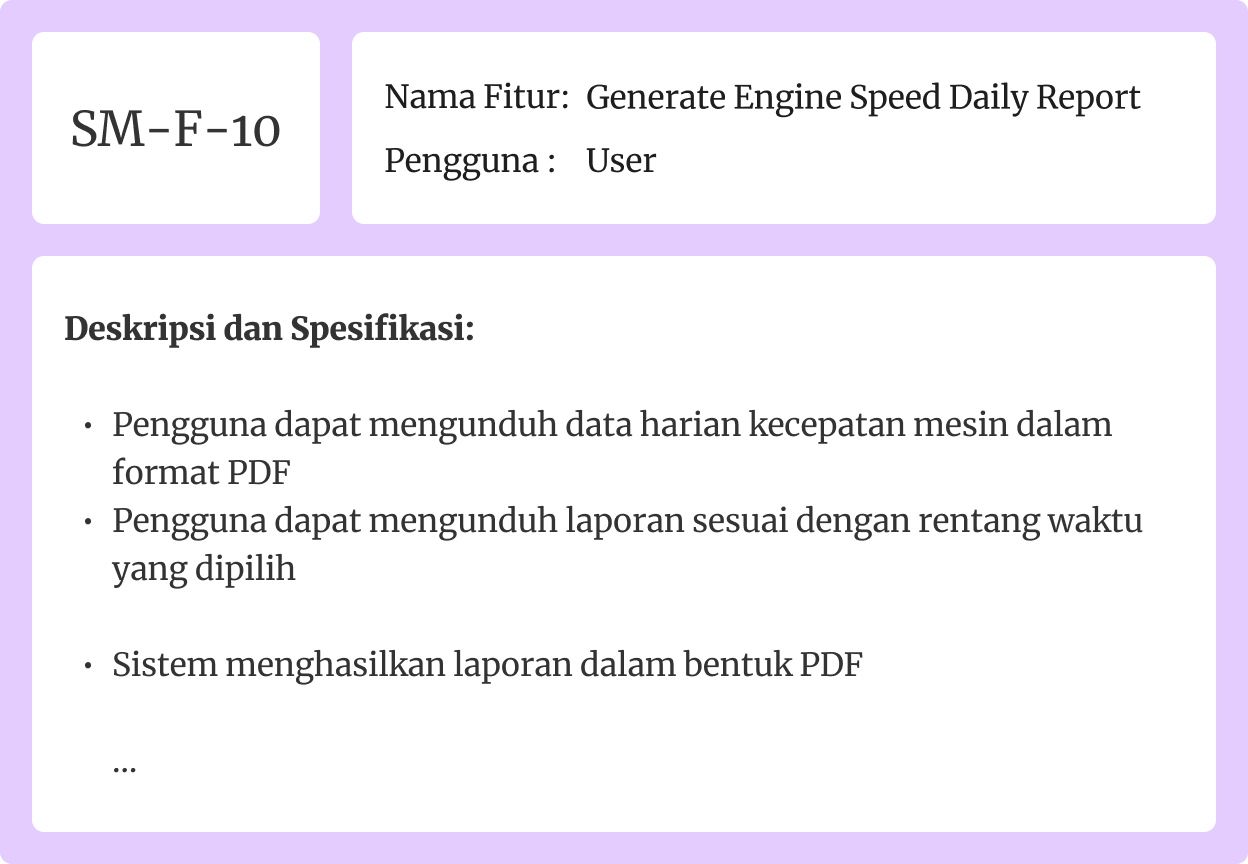
\includegraphics[width=.8\linewidth, center]{images/hasil/iterations/4/fr-generate-es-report.png}
%     \caption{Kebutuhan Fungsional Generate Engine Speed Daily Report}
%     \label{fig:fr-generate-es-report}
% \end{figure}

% \begin{figure}[!h]
%     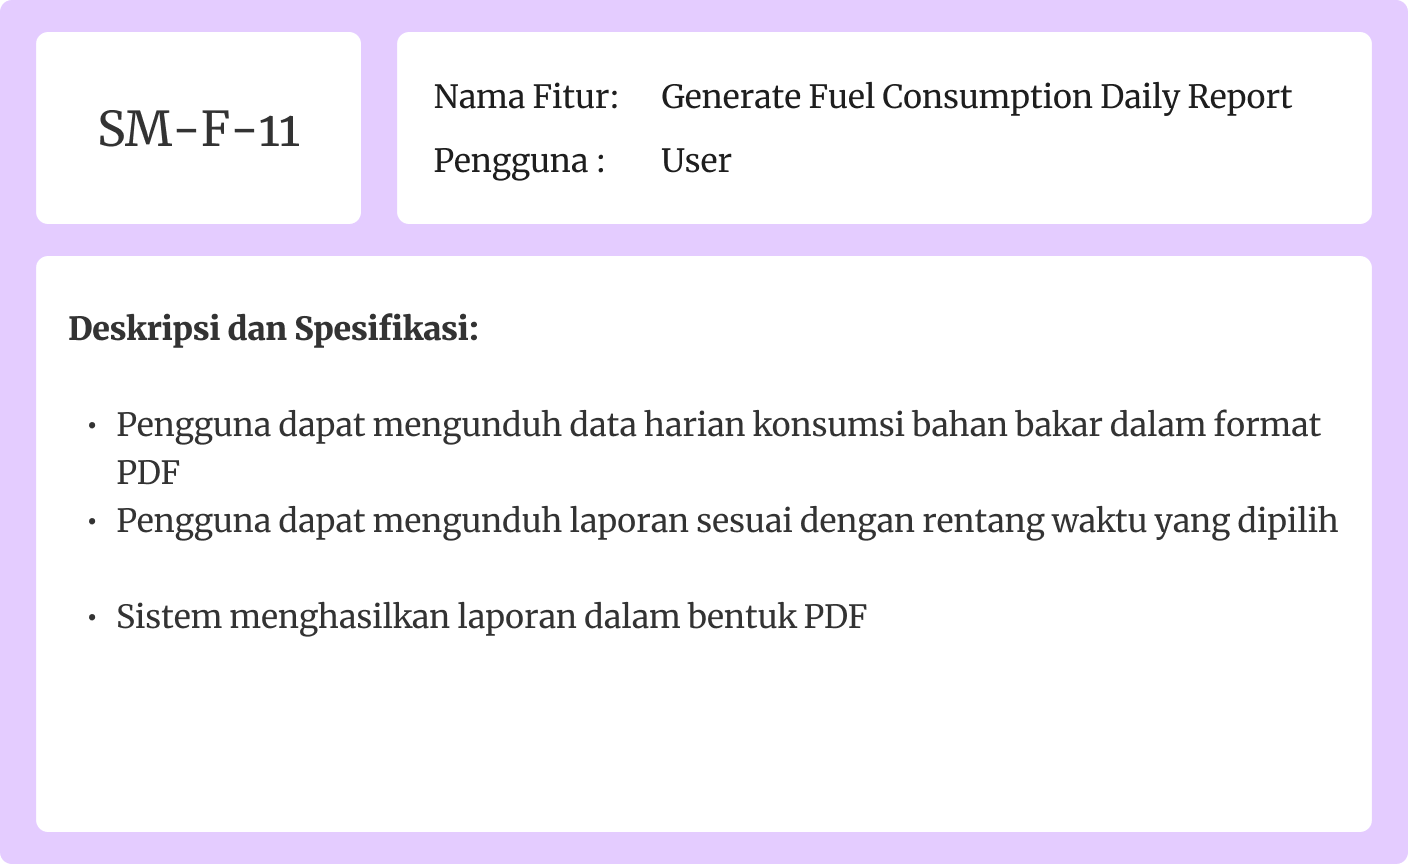
\includegraphics[width=.8\linewidth, center]{images/hasil/iterations/4/fr-generate-fuel-report.png}
%     \caption{Kebutuhan Fungsional Generate Fuel Consumption Daily Report}
%     \label{fig:fr-generate-fuel-report}
% \end{figure}

% \subsubsection{Desain}

% Pada tahap ini, dilakukan desain laporan bahan bakar yang kemudian dapat dibuat secara dinamis oleh sistem. Laporan kecepatan mesin dan bahan bakar dapat dilihat pada Gambar \ref{fig:es-report} dan Gambar \ref{fig:fc-report}.

% \begin{figure}[!h]
%     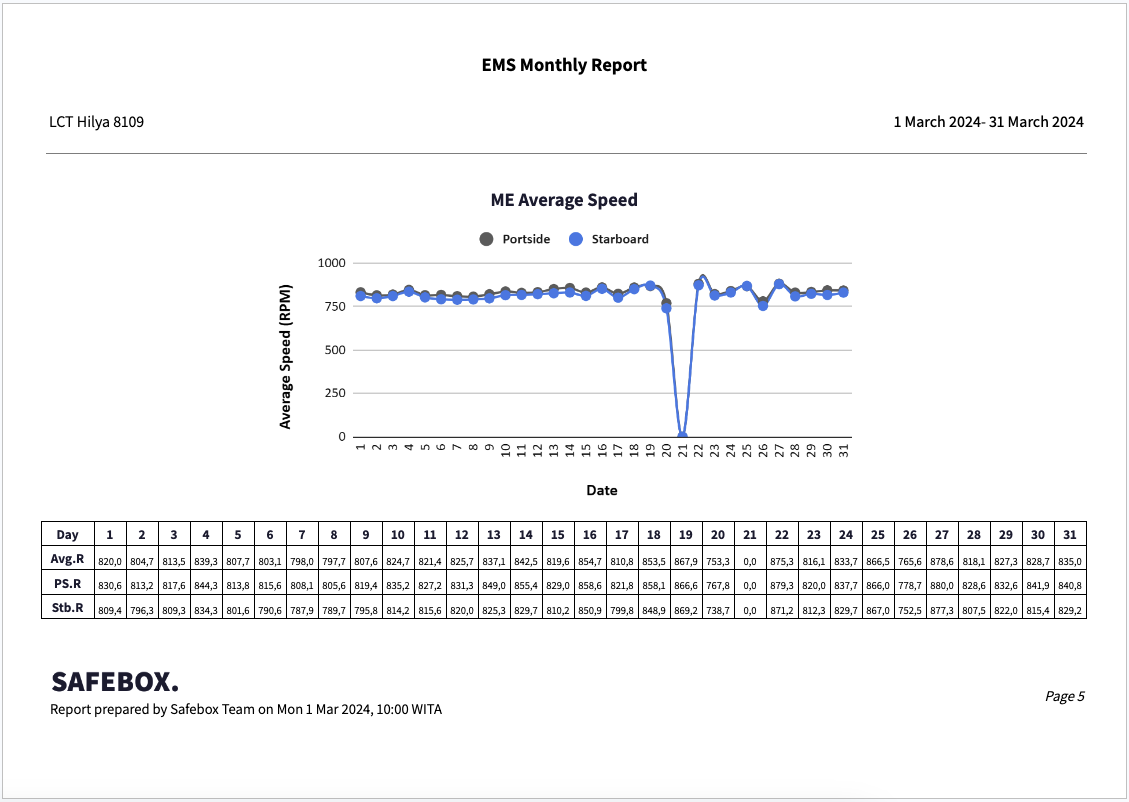
\includegraphics[width=1\linewidth, center]{images/hasil/iterations/4/es-report.png}
%     \caption{Contoh Laporan Kecepatan Mesin}
%     \label{fig:es-report}
% \end{figure}

% \begin{figure}[!h]
%     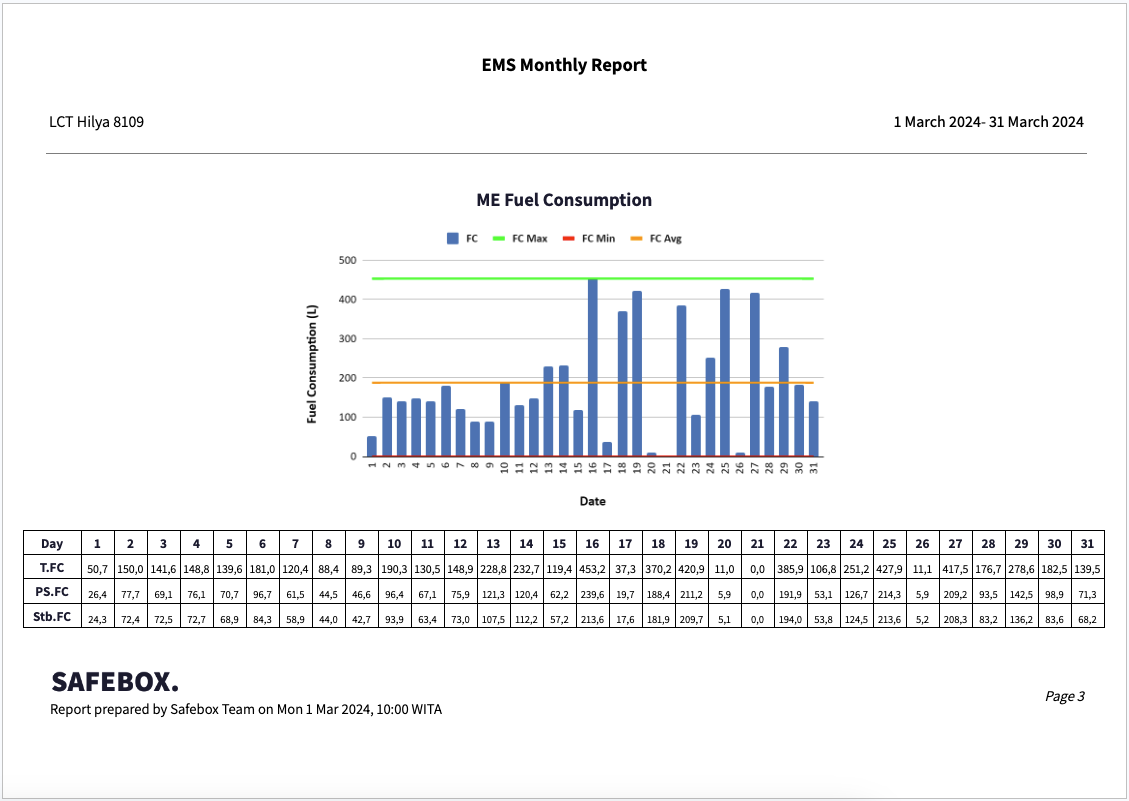
\includegraphics[width=1\linewidth, center]{images/hasil/iterations/4/fc-report.png}
%     \caption{Contoh Laporan Konsumsi Bahan Bakar}
%     \label{fig:fc-report}
% \end{figure}

% \newpage

% \subsubsection{Coding}
% \subsubsection{Whitebox Testing}

% \begin{landscape}
%     \subsubsection{Blackbox Testing}

%     \begin{longtable}[!h]
    {
            p{0.2\textwidth}
            p{0.3\textwidth}
            p{0.3\textwidth}
            p{0.3\textwidth}
            p{0.3\textwidth}
            p{0.15\textwidth}
    }
    \caption{\textit{Blackbox Testing Generate Engine Speed Daily Report}}
    \label{tab:it4-blackbox-generate-es-report} \\

    \hline
        \bfseries \textit{Test Code} &
        \bfseries \textit{Test Case} &
        \bfseries \textit{Test Steps} &
        \bfseries \textit{Expected Result} &
        \bfseries \textit{Actual Result} &
        \bfseries \textit{Pass/Fail} \\ [0.5ex]
    \hline

    \endfirsthead

    \hline
        \bfseries \textit{Test Code} &
        \bfseries \textit{Test Case} &
        \bfseries \textit{Test Steps} &
        \bfseries \textit{Expected Result} &
        \bfseries \textit{Actual Result} &
        \bfseries \textit{Pass/Fail} \\ [0.5ex]
    \hline
    \endhead % all the lines above this will be repeated on every page
    \hline

    \csvreader[
        late after line=\\,
        before reading={\catcode`\#=12},after reading={\catcode`\#=6}
    ]{tables/hasil/iterations/4/blackbox/generate-es-report.csv}
    {1=\code, 2=\case, 3=\step, 4=\expect, 5=\actual, 6=\status}
    {\code & \case & \step & \expect & \actual & \status} \\

    \bottomrule
\end{longtable}
%     \newpage
%     \begin{longtable}[!h]
    {
            p{0.2\textwidth}
            p{0.3\textwidth}
            p{0.3\textwidth}
            p{0.3\textwidth}
            p{0.3\textwidth}
            p{0.15\textwidth}
    }
    \caption{\textit{Blackbox Testing Generate Fuel Consumption Daily Report}}
    \label{tab:it4-blackbox-generate-fuel-report} \\

    \hline
        \bfseries \textit{Test Code} &
        \bfseries \textit{Test Case} &
        \bfseries \textit{Test Steps} &
        \bfseries \textit{Expected Result} &
        \bfseries \textit{Actual Result} &
        \bfseries \textit{Pass/Fail} \\ [0.5ex]
    \hline

    \endfirsthead

    \hline
        \bfseries \textit{Test Code} &
        \bfseries \textit{Test Case} &
        \bfseries \textit{Test Steps} &
        \bfseries \textit{Expected Result} &
        \bfseries \textit{Actual Result} &
        \bfseries \textit{Pass/Fail} \\ [0.5ex]
    \hline
    \endhead % all the lines above this will be repeated on every page
    \hline

    \csvreader[
        late after line=\\,
        before reading={\catcode`\#=12},after reading={\catcode`\#=6}
    ]{tables/hasil/iterations/4/blackbox/generate-fuel-report.csv}
    {1=\code, 2=\case, 3=\step, 4=\expect, 5=\actual, 6=\status}
    {\code & \case & \step & \expect & \actual & \status} \\

    \bottomrule
\end{longtable}
% \end{landscape}

% \subsection{Iterasi 5}

% \subsubsection{Analisis}

% Pada iterasi terakhir, dilakukan pengembangan fitur ekspor data yang terdapat pada Halaman Data Log, autentikasi sistem, Halaman OP41 Report, dan Halaman Overview. Kebutuhan fungsional dapat dilihat pada Gambar \ref{fig:fr-export-data} hingga Gambar \ref{fig:fr-op41}

% \begin{figure}[!h]
%     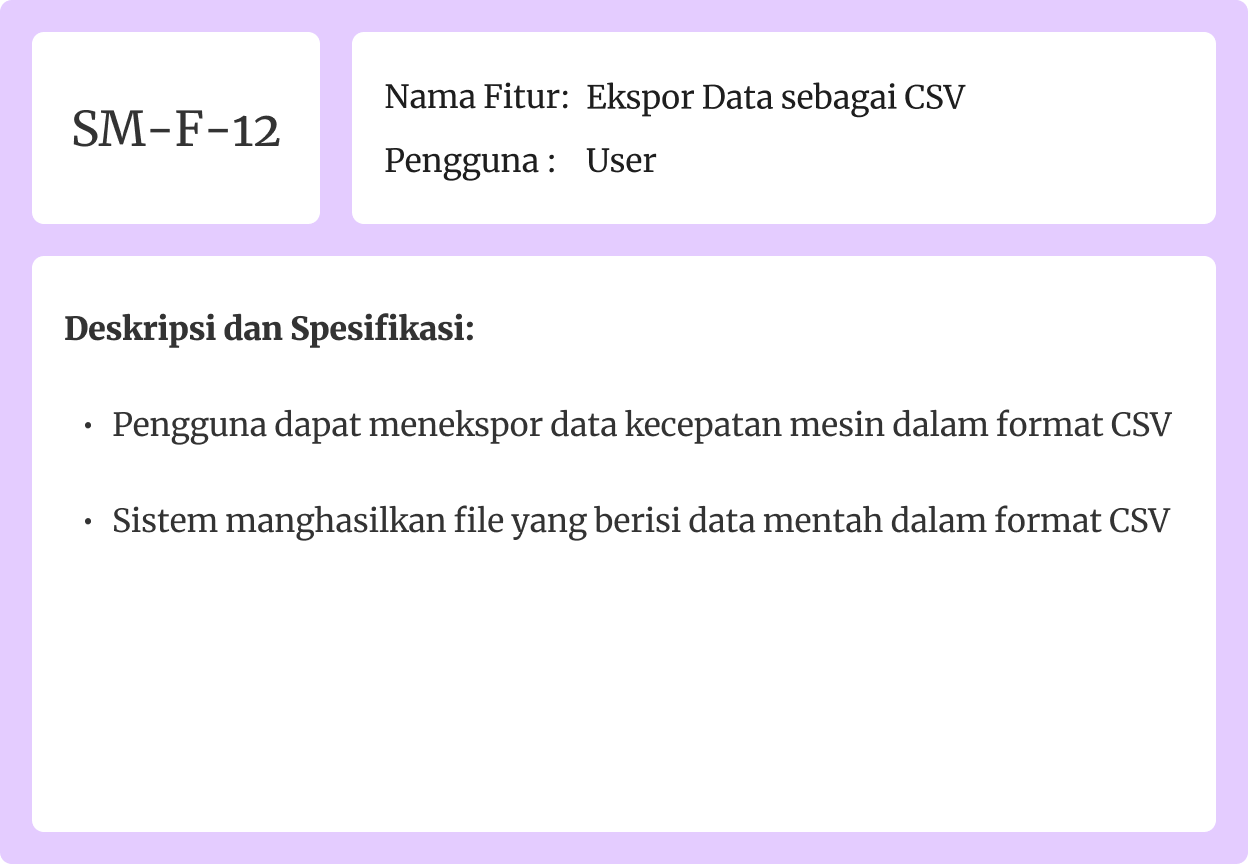
\includegraphics[width=1\linewidth, center]{images/hasil/iterations/5/fr-export-data.png}
%     \caption{Kebutuhan Fungsional Ekspor Data}
%     \label{fig:fr-export-data}
% \end{figure}

% \begin{figure}[!h]
%     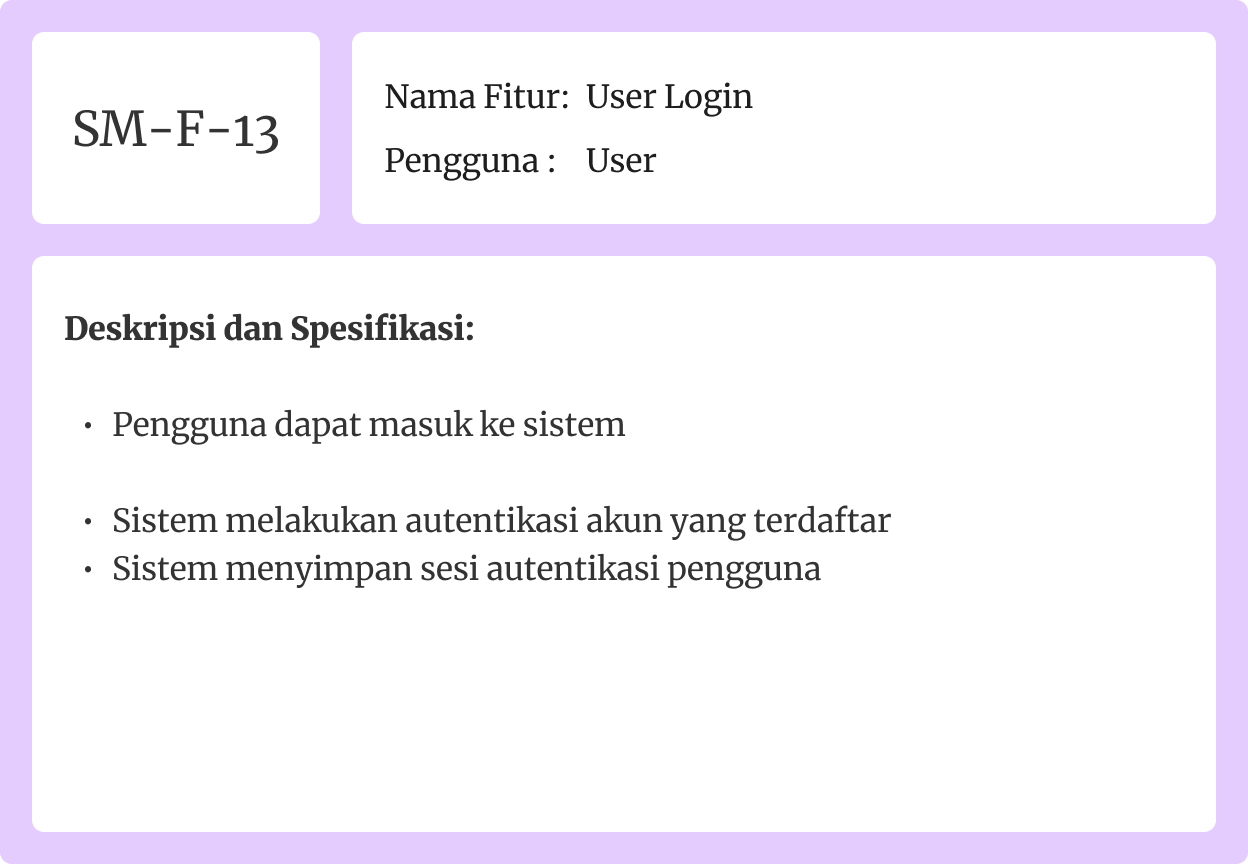
\includegraphics[width=1\linewidth, center]{images/hasil/iterations/5/fr-login-user.png}
%     \caption{Kebutuhan Fungsional User Login}
%     \label{fig:fr-login-user}
% \end{figure}

% \begin{figure}[!h]
%     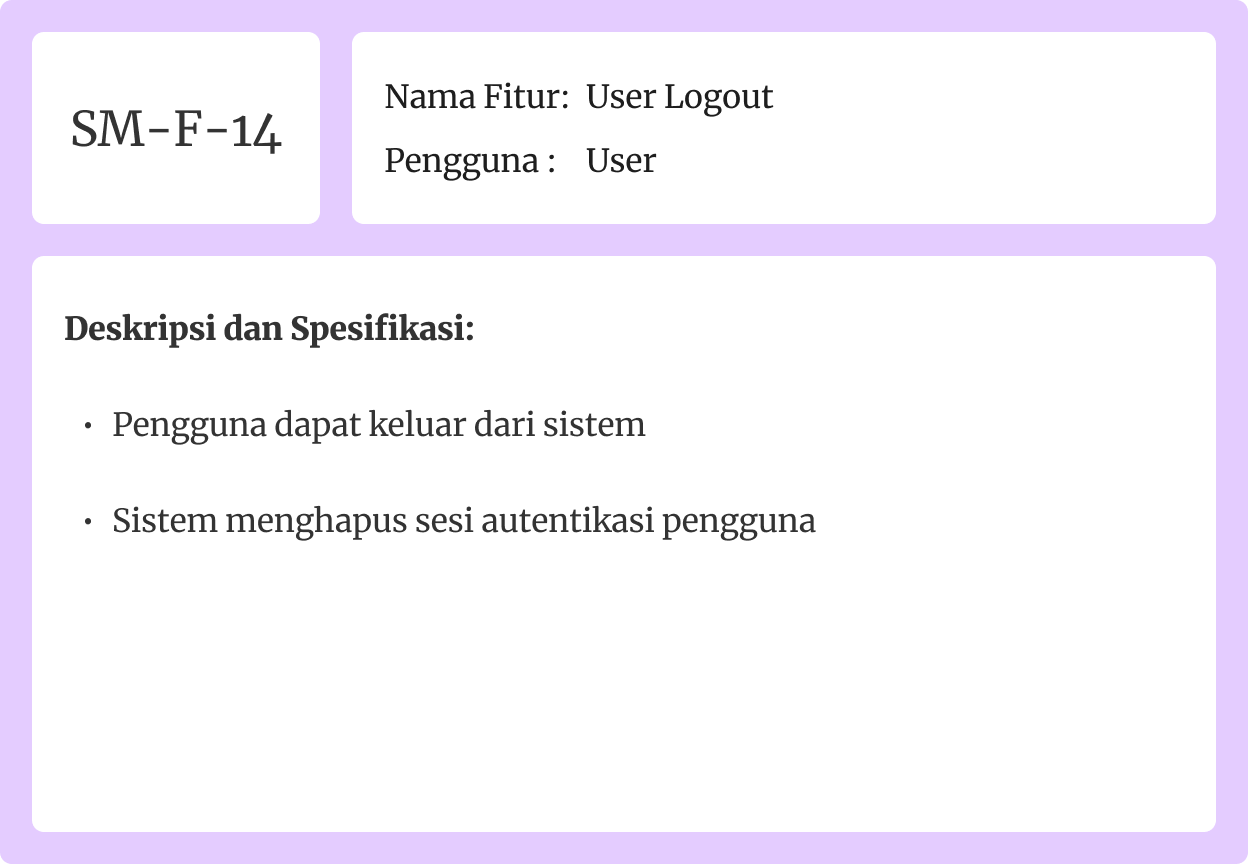
\includegraphics[width=1\linewidth, center]{images/hasil/iterations/5/fr-logout-user.png}
%     \caption{Kebutuhan Fungsional User Logout}
%     \label{fig:fr-logout-user}
% \end{figure}

% \begin{figure}[!h]
%     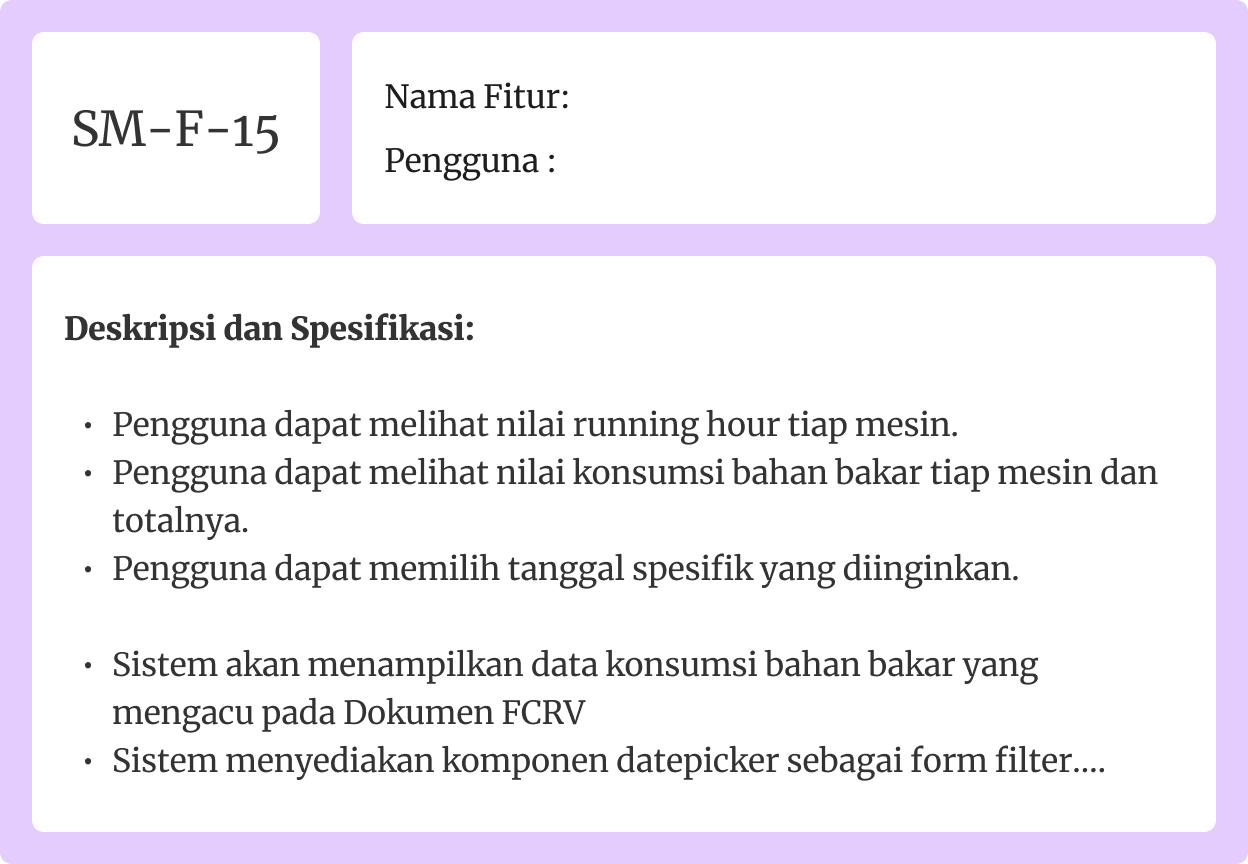
\includegraphics[width=1\linewidth, center]{images/hasil/iterations/5/fr-op41.png}
%     \caption{Kebutuhan Fungsional OP41 Report}
%     \label{fig:fr-op41}
% \end{figure}

% \newpage

% \subsubsection{Desain}

% Dilakukan desain pada Halaman Login, OP41 Report, dan Overview yang dapat dilihat pada Gambar \ref{fig:lofi-login}, Gambar \ref{fig:lofi-op41} dan Gambar \ref{lif-} secara berturut-turut.

% \begin{figure}[!h]
%     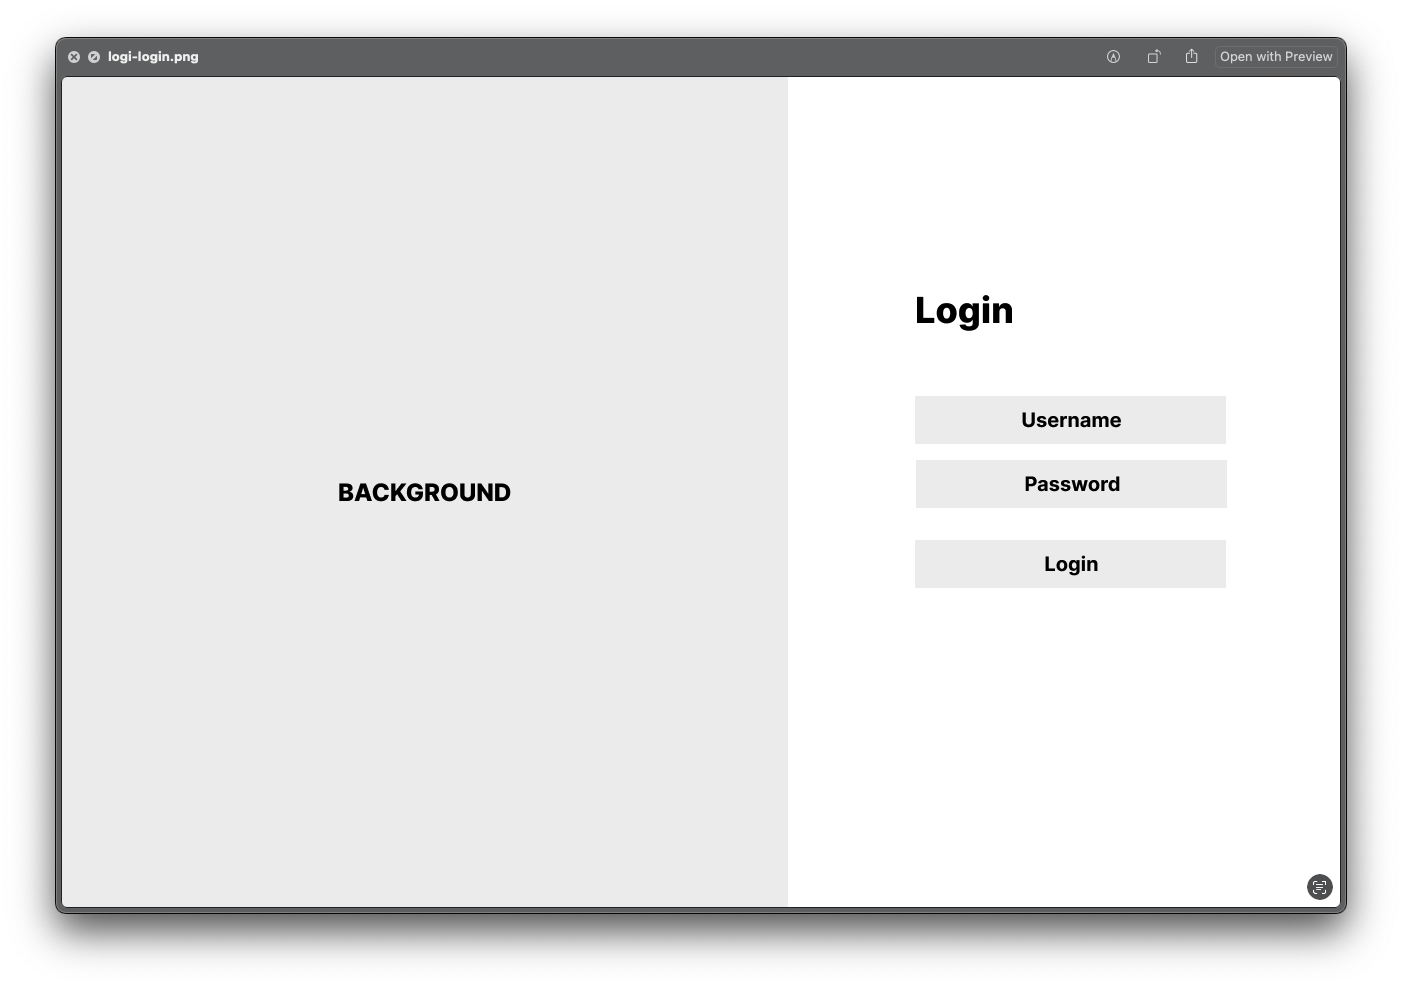
\includegraphics[width=1.05\linewidth, center]{images/hasil/iterations/5/lofi-login.png}
%     \caption{Wireframe Halaman Login}
%     \label{fig:lofi-login}
% \end{figure}

% \begin{figure}[!h]
%     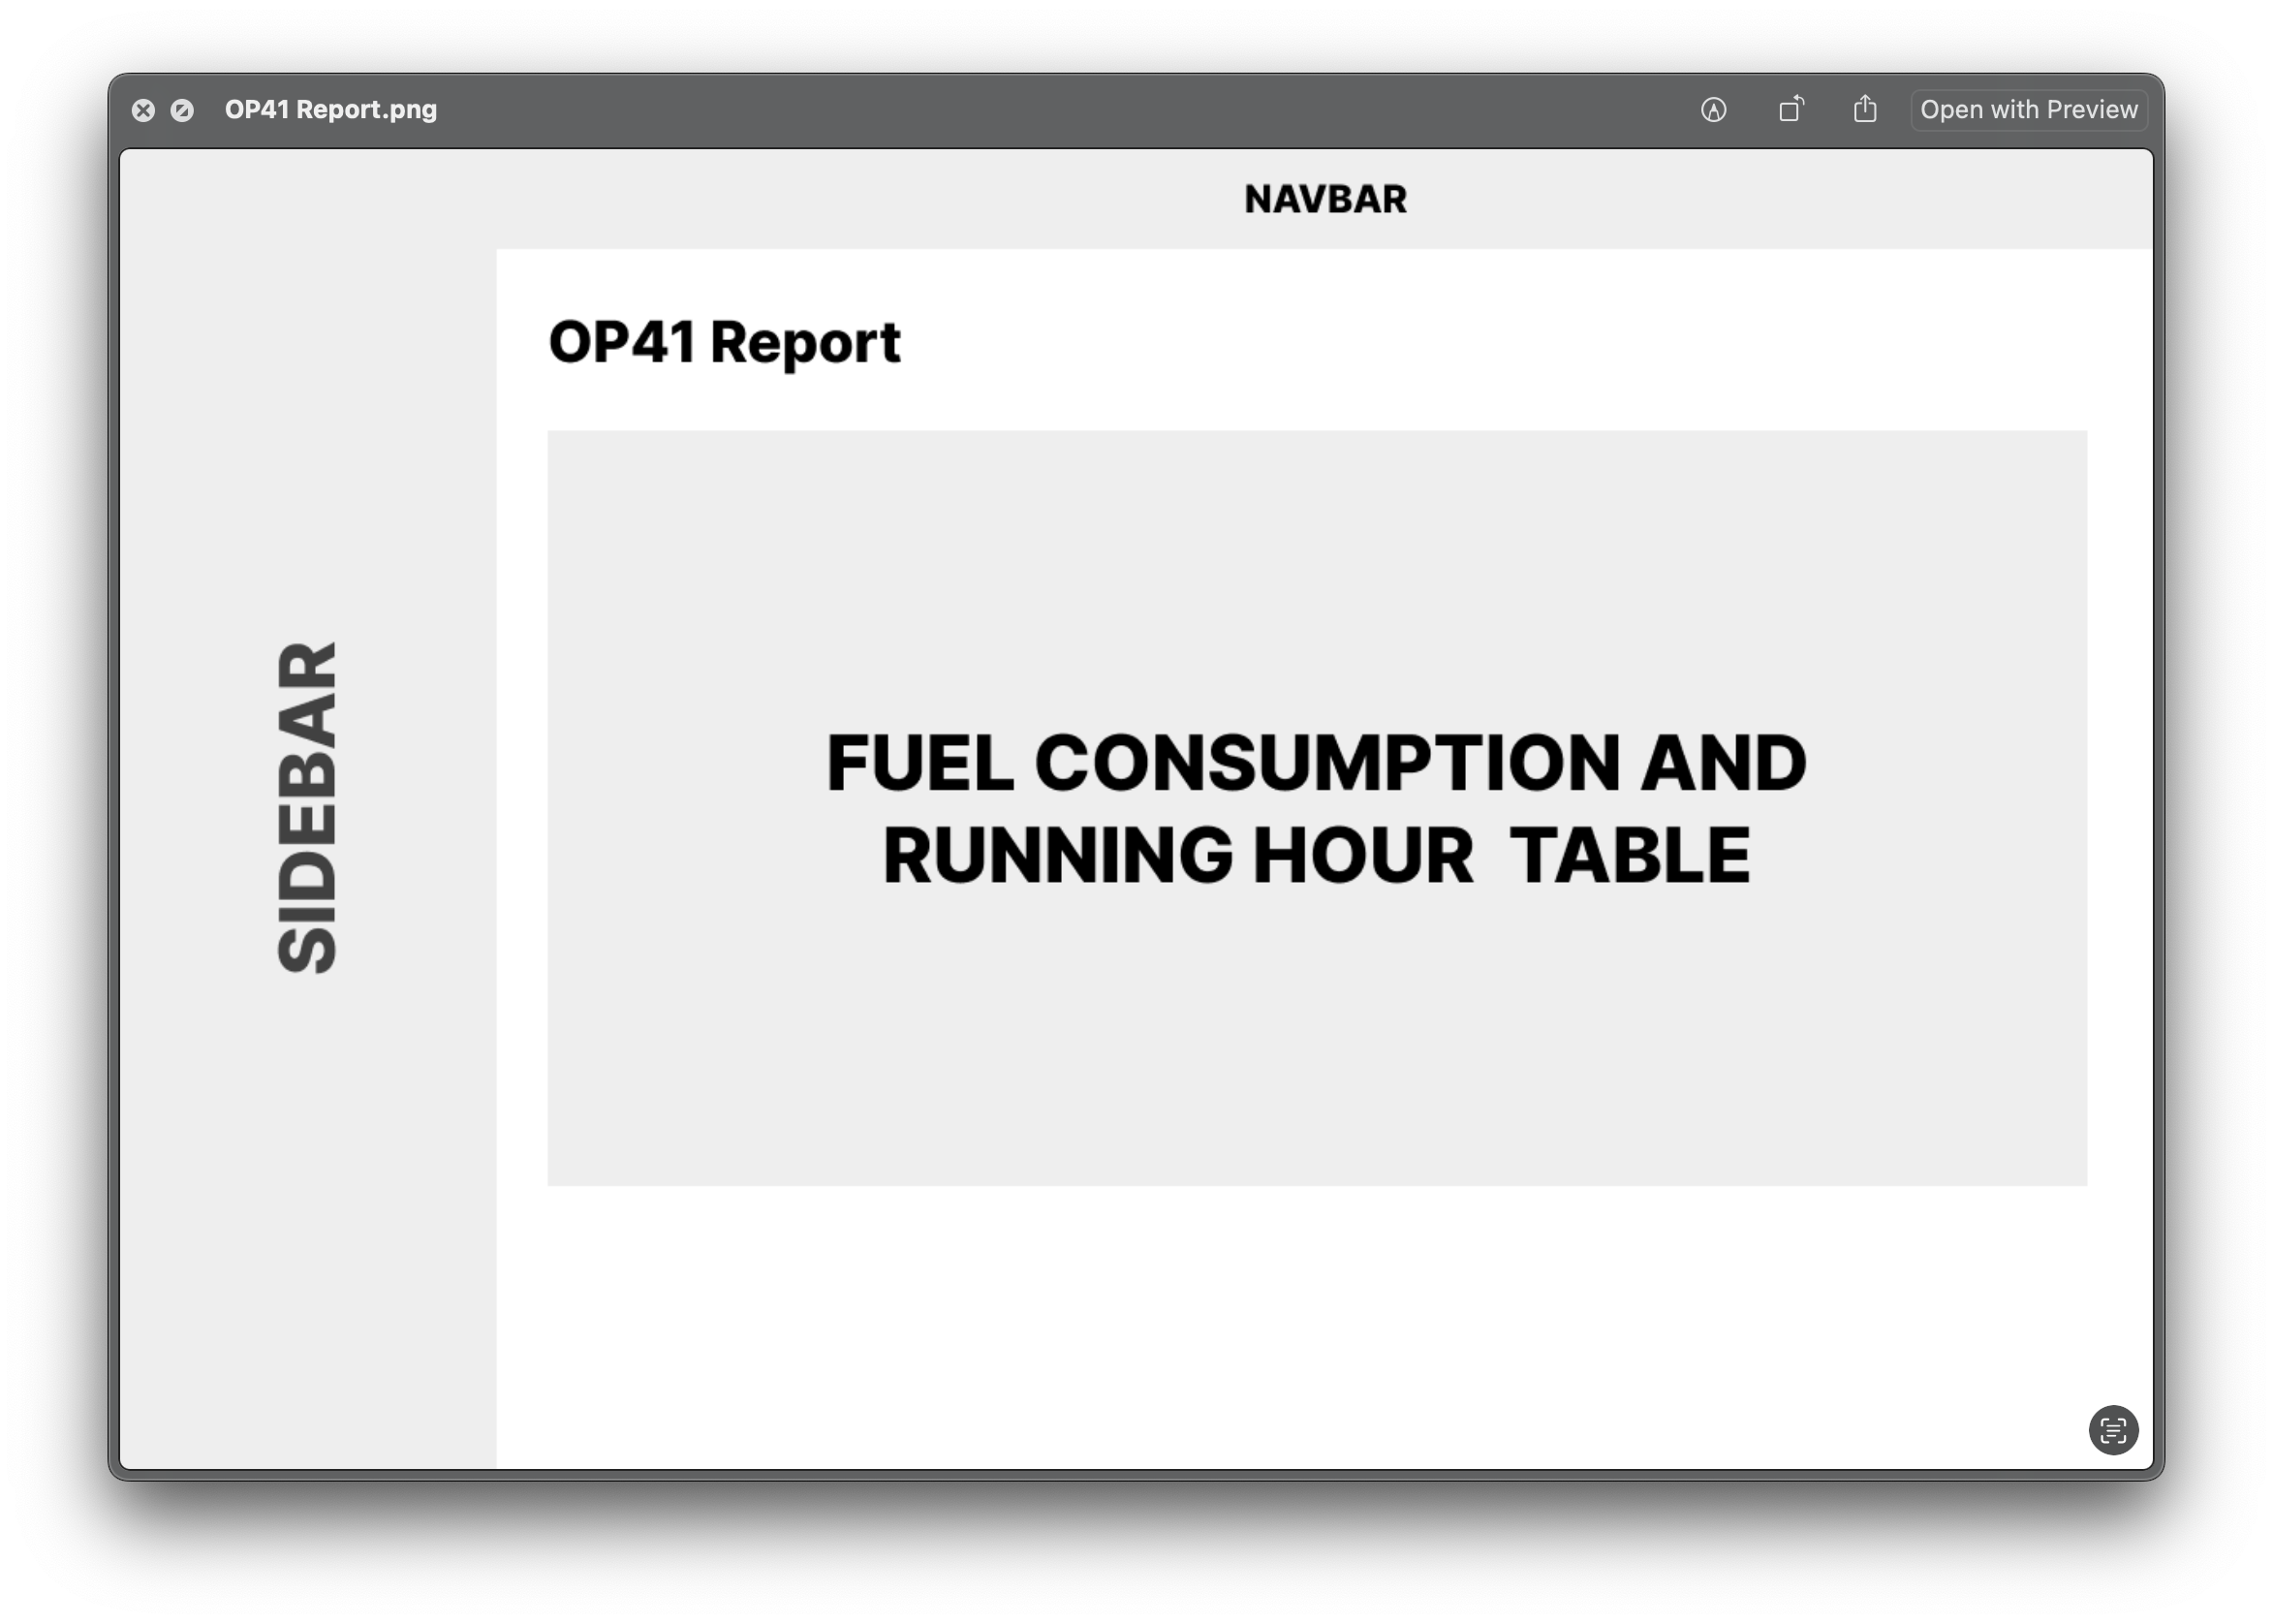
\includegraphics[width=1.05\linewidth, center]{images/hasil/iterations/1/lofi-op41.png}
%     \caption{Wireframe Halaman OP41 Report}
%     \label{fig:lofi-op41}
% \end{figure}

% \begin{figure}[!h]
%     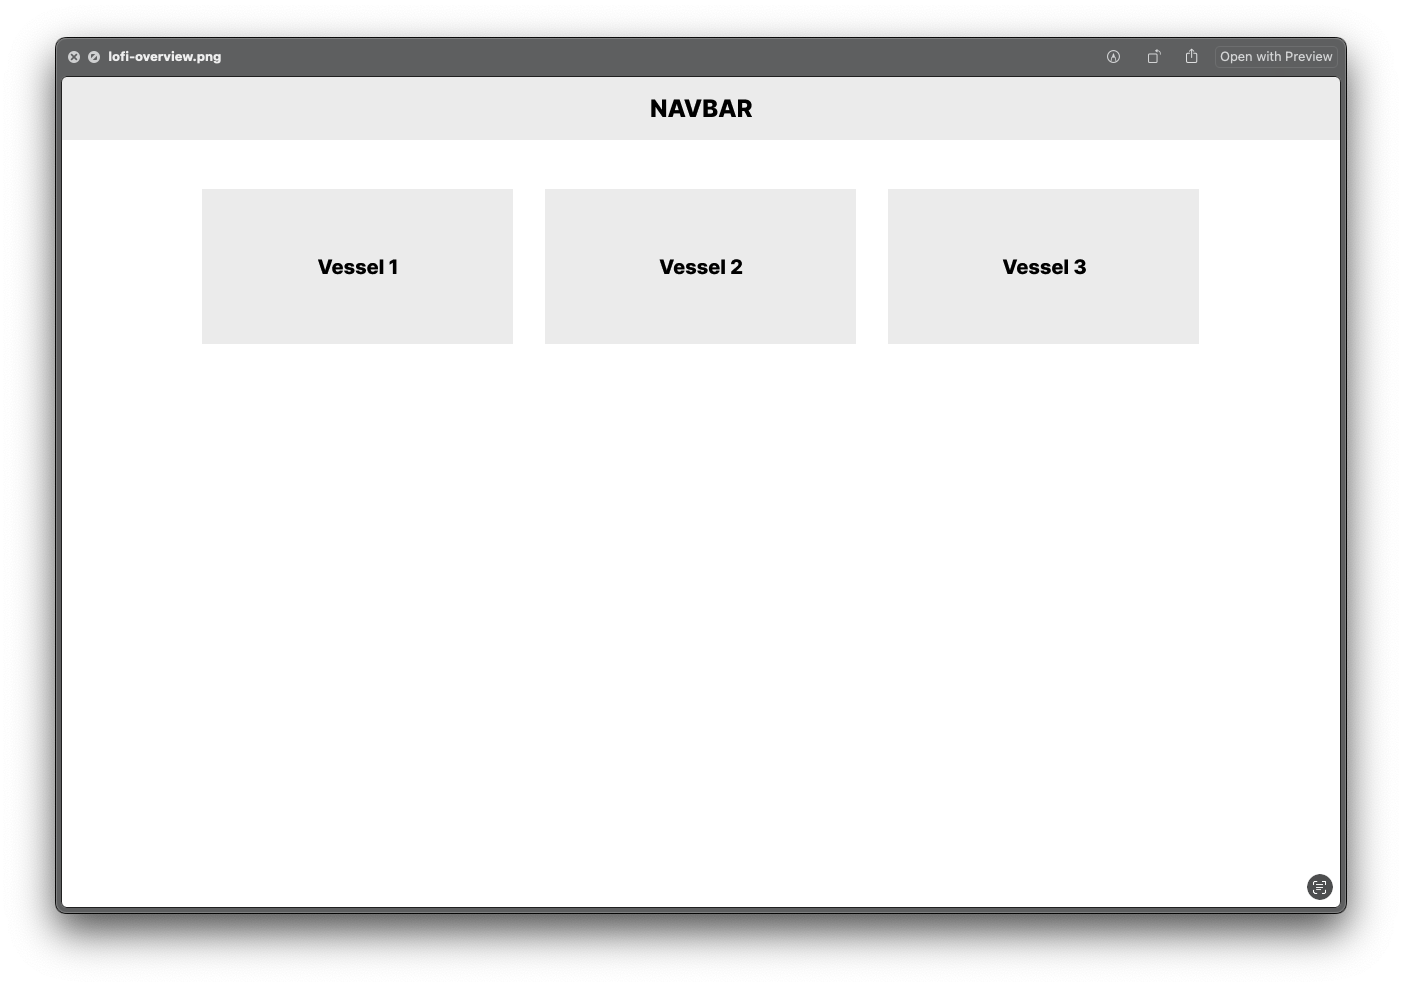
\includegraphics[width=1.05\linewidth, center]{images/hasil/iterations/5/lofi-overview.png}
%     \caption{Wireframe Halaman Overview}
%     \label{fig:lofi-overview}
% \end{figure}

% \newpage

% \subsubsection{Coding}

% Halaman OP41 memuat informasi running hour dan fuel consumption pada tiap kategori operasi berdasarkan Dokumen FCRV yang dapat menjadi acuan awak kapal untuk mengisi laporan. Jika data belum masuk semua maka ditampilkan alert agar awak kapal tidak mengisi laporan sebelum data pada hari tersebut telah tersinkron. Halaman OP41 dapat dilihat pada Gambar \ref{fig:fe-op41}.

% \begin{figure}[!h]
%     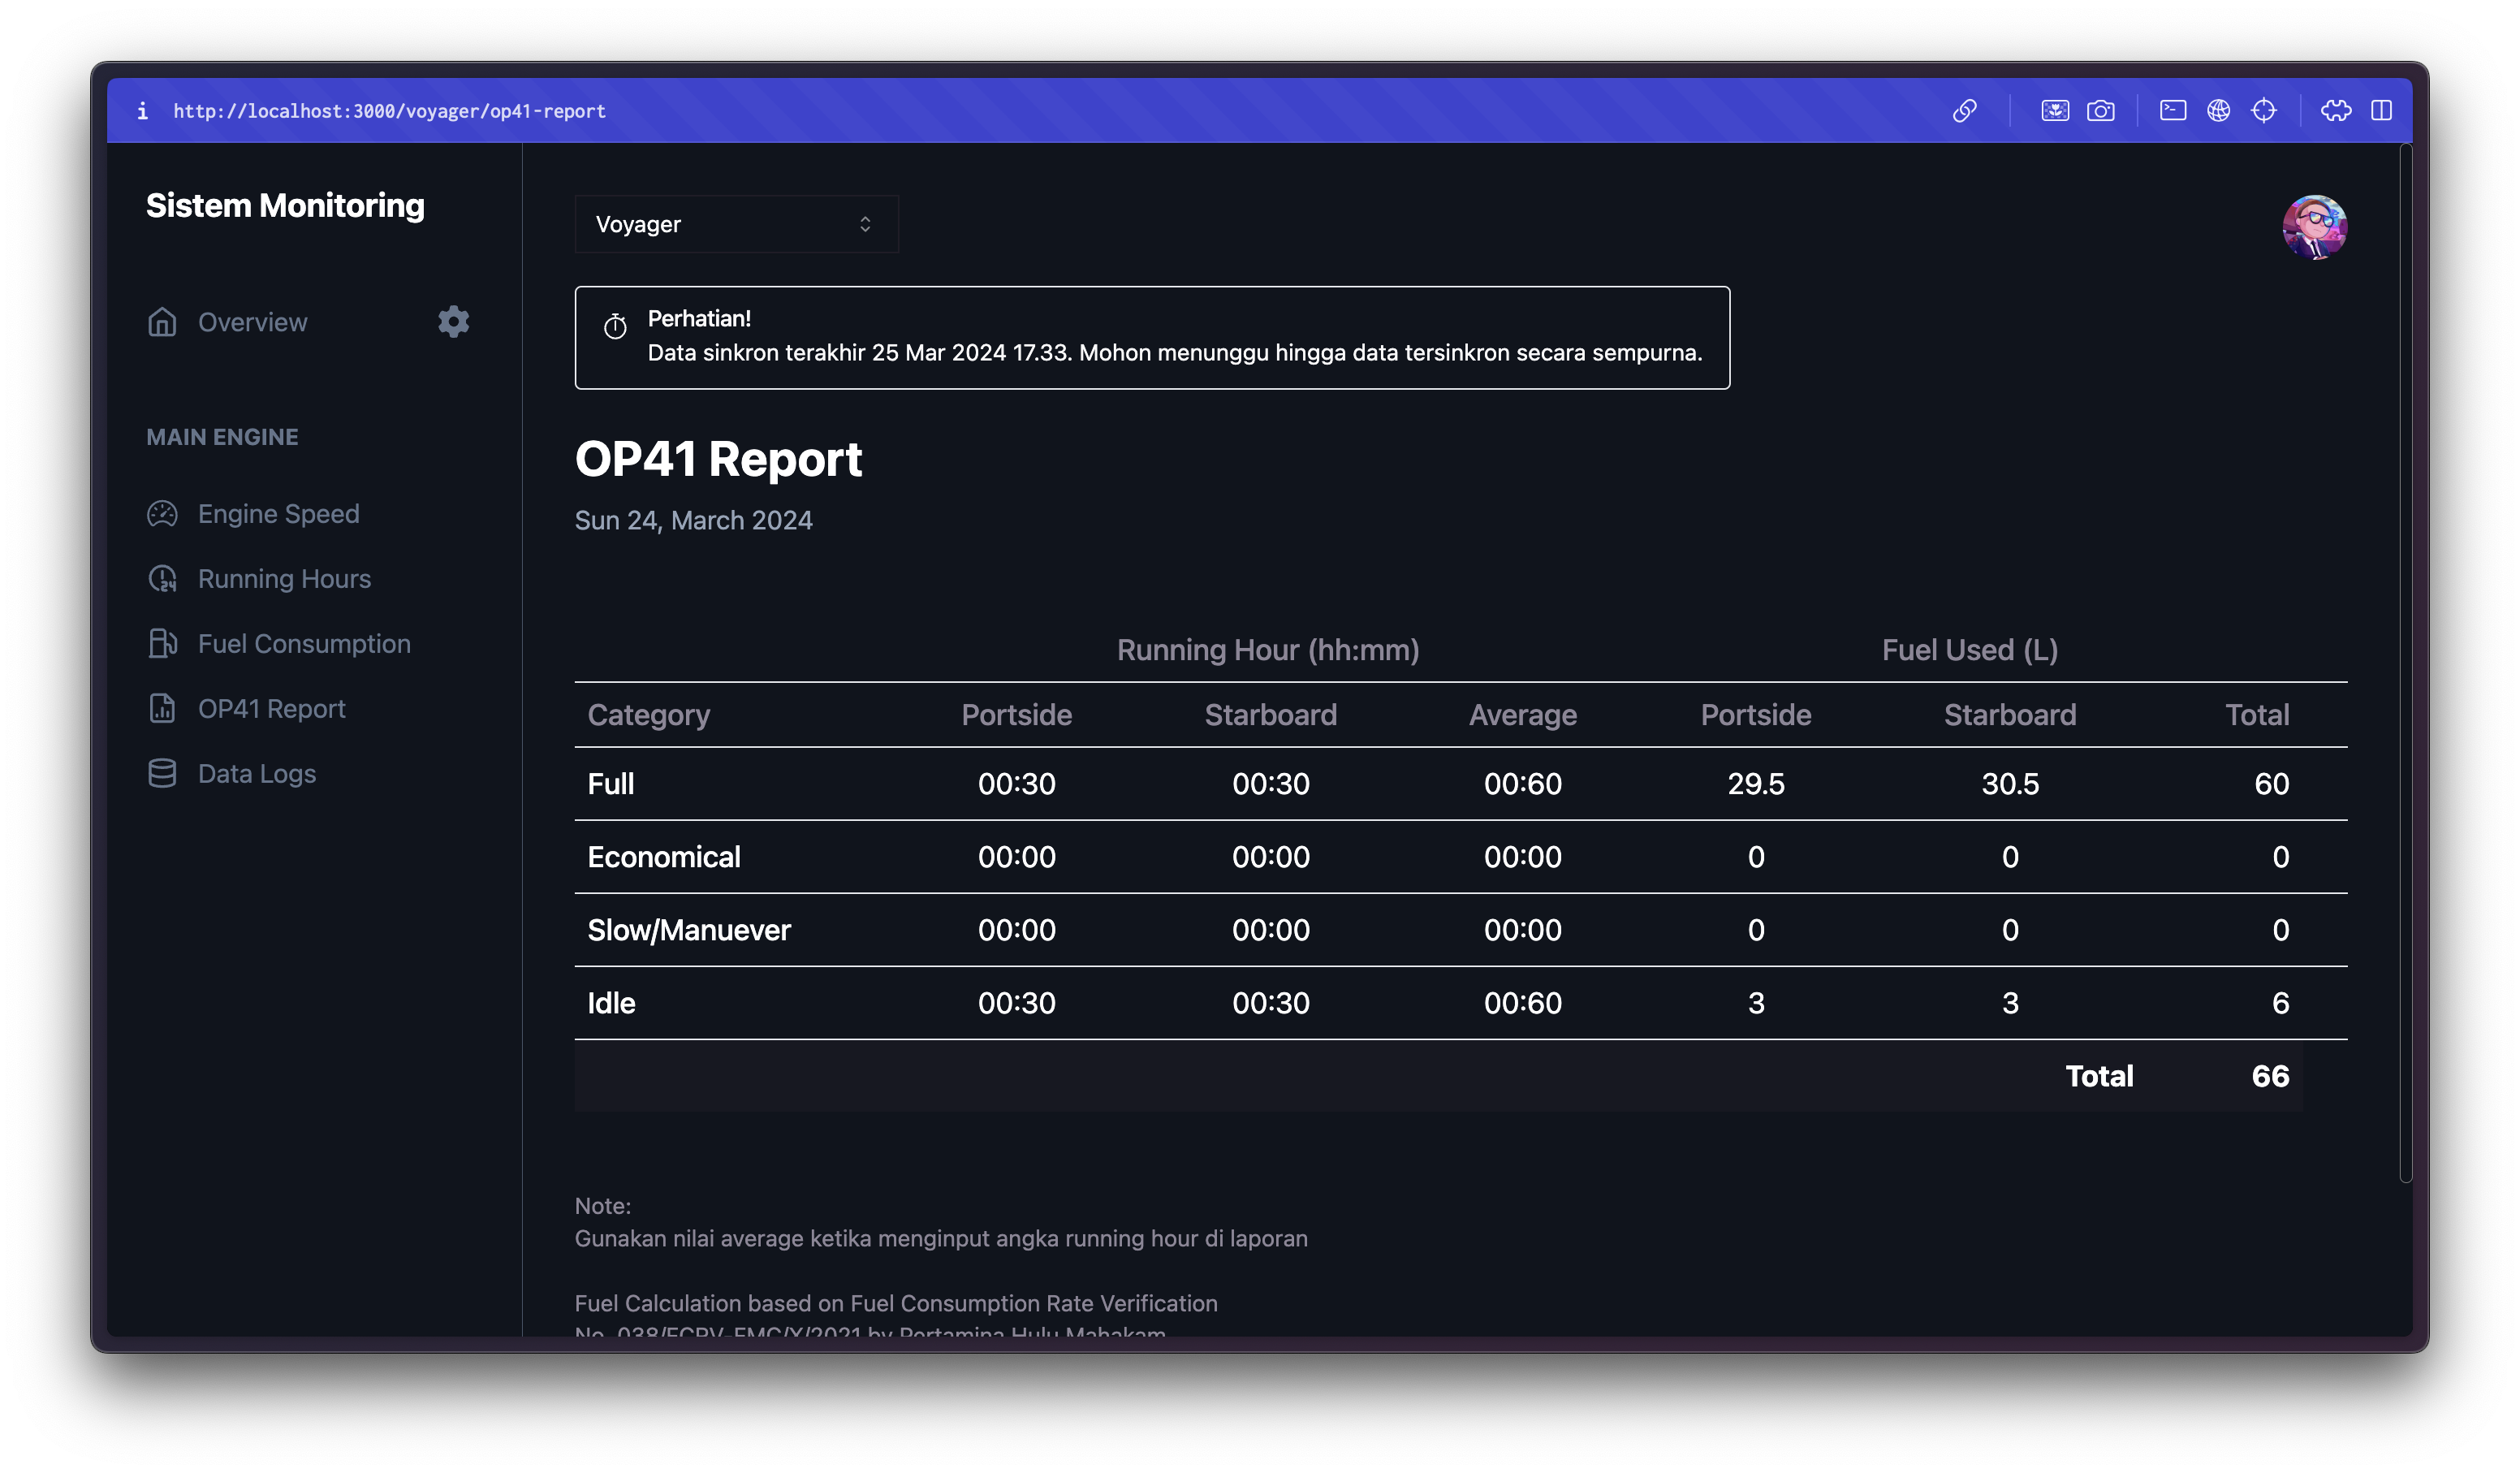
\includegraphics[width=1\linewidth, center]{images/hasil/iterations/5/fe-op41.png}
%     \caption{Frontend OP41 Report}
%     \label{fig:fe-op41}
% \end{figure}

% \newpage

% \subsubsection{Whitebox Testing}

% \begin{landscape}
%     \subsubsection{Blackbox Testing}

%     \begin{longtable}[!h]
    {
            p{0.2\textwidth}
            p{0.3\textwidth}
            p{0.3\textwidth}
            p{0.3\textwidth}
            p{0.3\textwidth}
            p{0.15\textwidth}
    }
    \caption{Blackbox Testing Ekspor Data Log Kecepatan Mesin}
    \label{tab:it4-blackbox-generate-es-report} \\

    \hline
        \bfseries \textit{Test Code} &
        \bfseries \textit{Test Case} &
        \bfseries \textit{Test Steps} &
        \bfseries \textit{Expected Result} &
        \bfseries \textit{Actual Result} &
        \bfseries \textit{Pass/Fail} \\ [0.5ex]
    \hline

    \endfirsthead

    \hline
        \bfseries \textit{Test Code} &
        \bfseries \textit{Test Case} &
        \bfseries \textit{Test Steps} &
        \bfseries \textit{Expected Result} &
        \bfseries \textit{Actual Result} &
        \bfseries \textit{Pass/Fail} \\ [0.5ex]
    \hline
    \endhead % all the lines above this will be repeated on every page
    \hline

    \csvreader[
        late after line=\\,
        before reading={\catcode`\#=12},after reading={\catcode`\#=6}
    ]{tables/hasil/iterations/5/blackbox/export-data.csv}
    {1=\code, 2=\case, 3=\step, 4=\expect, 5=\actual, 6=\status}
    {\code & \case & \step & \expect & \actual & \status} \\

    \bottomrule
\end{longtable}
%     \newpage
%     \begin{longtable}[!h]
    {
            p{0.2\textwidth}
            p{0.3\textwidth}
            p{0.3\textwidth}
            p{0.3\textwidth}
            p{0.3\textwidth}
            p{0.15\textwidth}
    }
    \caption{Blackbox Testing Halaman Autentikasi}
    \label{tab:it3-blackbox-auth-admin} \\

    \hline
        \bfseries \textit{Test Code} &
        \bfseries \textit{Test Case} &
        \bfseries \textit{Test Steps} &
        \bfseries \textit{Expected Result} &
        \bfseries \textit{Actual Result} &
        \bfseries \textit{Pass/Fail} \\ [0.5ex]
    \hline

    \endfirsthead

    \hline
        \bfseries \textit{Test Code} &
        \bfseries \textit{Test Case} &
        \bfseries \textit{Test Steps} &
        \bfseries \textit{Expected Result} &
        \bfseries \textit{Actual Result} &
        \bfseries \textit{Pass/Fail} \\ [0.5ex]
    \hline
    \endhead % all the lines above this will be repeated on every page
    \hline

    \csvreader[
        late after line=\\,
        before reading={\catcode`\#=12},after reading={\catcode`\#=6}
    ]{tables/hasil/iterations/3/blackbox/autentikasi.csv}
    {1=\code, 2=\case, 3=\step, 4=\expect, 5=\actual, 6=\status}
    {\code & \case & \step & \expect & \actual & \status} \\

    \bottomrule
\end{longtable}

% \end{landscape}